% Options for packages loaded elsewhere
\PassOptionsToPackage{unicode}{hyperref}
\PassOptionsToPackage{hyphens}{url}
%
\documentclass[
]{article}
\usepackage{amsmath,amssymb}
\usepackage{lmodern}
\usepackage{ifxetex,ifluatex}
\ifnum 0\ifxetex 1\fi\ifluatex 1\fi=0 % if pdftex
  \usepackage[T1]{fontenc}
  \usepackage[utf8]{inputenc}
  \usepackage{textcomp} % provide euro and other symbols
\else % if luatex or xetex
  \usepackage{unicode-math}
  \defaultfontfeatures{Scale=MatchLowercase}
  \defaultfontfeatures[\rmfamily]{Ligatures=TeX,Scale=1}
\fi
% Use upquote if available, for straight quotes in verbatim environments
\IfFileExists{upquote.sty}{\usepackage{upquote}}{}
\IfFileExists{microtype.sty}{% use microtype if available
  \usepackage[]{microtype}
  \UseMicrotypeSet[protrusion]{basicmath} % disable protrusion for tt fonts
}{}
\makeatletter
\@ifundefined{KOMAClassName}{% if non-KOMA class
  \IfFileExists{parskip.sty}{%
    \usepackage{parskip}
  }{% else
    \setlength{\parindent}{0pt}
    \setlength{\parskip}{6pt plus 2pt minus 1pt}}
}{% if KOMA class
  \KOMAoptions{parskip=half}}
\makeatother
\usepackage{xcolor}
\IfFileExists{xurl.sty}{\usepackage{xurl}}{} % add URL line breaks if available
\IfFileExists{bookmark.sty}{\usepackage{bookmark}}{\usepackage{hyperref}}
\hypersetup{
  pdftitle={Extending the open monitoring of open science},
  pdfkeywords={clinical trials, journal business models, observational
studies, open access, open science, scientometrics, unpaywall},
  hidelinks,
  pdfcreator={LaTeX via pandoc}}
\urlstyle{same} % disable monospaced font for URLs
\usepackage[left=3cm, right=3cm, top=3cm, bottom=3cm]{geometry}
\usepackage{graphicx}
\makeatletter
\def\maxwidth{\ifdim\Gin@nat@width>\linewidth\linewidth\else\Gin@nat@width\fi}
\def\maxheight{\ifdim\Gin@nat@height>\textheight\textheight\else\Gin@nat@height\fi}
\makeatother
% Scale images if necessary, so that they will not overflow the page
% margins by default, and it is still possible to overwrite the defaults
% using explicit options in \includegraphics[width, height, ...]{}
\setkeys{Gin}{width=\maxwidth,height=\maxheight,keepaspectratio}
% Set default figure placement to htbp
\makeatletter
\def\fps@figure{htbp}
\makeatother
\setlength{\emergencystretch}{3em} % prevent overfull lines
\providecommand{\tightlist}{%
  \setlength{\itemsep}{0pt}\setlength{\parskip}{0pt}}
\setcounter{secnumdepth}{-\maxdimen} % remove section numbering
\ifluatex
  \usepackage{selnolig}  % disable illegal ligatures
\fi
\newlength{\cslhangindent}
\setlength{\cslhangindent}{1.5em}
\newlength{\csllabelwidth}
\setlength{\csllabelwidth}{3em}
\newenvironment{CSLReferences}[2] % #1 hanging-ident, #2 entry spacing
 {% don't indent paragraphs
  \setlength{\parindent}{0pt}
  % turn on hanging indent if param 1 is 1
  \ifodd #1 \everypar{\setlength{\hangindent}{\cslhangindent}}\ignorespaces\fi
  % set entry spacing
  \ifnum #2 > 0
  \setlength{\parskip}{#2\baselineskip}
  \fi
 }%
 {}
\usepackage{calc}
\newcommand{\CSLBlock}[1]{#1\hfill\break}
\newcommand{\CSLLeftMargin}[1]{\parbox[t]{\csllabelwidth}{#1}}
\newcommand{\CSLRightInline}[1]{\parbox[t]{\linewidth - \csllabelwidth}{#1}\break}
\newcommand{\CSLIndent}[1]{\hspace{\cslhangindent}#1}
% for compatibility with pandoc 2.10
\newenvironment{cslreferences}%
  {\setlength{\parindent}{0pt}%
  \everypar{\setlength{\hangindent}{\cslhangindent}}\ignorespaces}%
  {\par}

\title{Extending the open monitoring of open science}
\usepackage{etoolbox}
\makeatletter
\providecommand{\subtitle}[1]{% add subtitle to \maketitle
  \apptocmd{\@title}{\par {\large #1 \par}}{}{}
}
\makeatother
\subtitle{A new framework for the French Open Science Monitor (BSO)}
\usepackage{authblk}
\author[%
  2%
  ]{%
  Laetitia Bracco%
  %
  %
}
\author[%
  1%
  ]{%
  Anne L'Hôte%
  %
  %
}
\author[%
  1%
  ]{%
  Eric Jeangirard%
  %
  %
}
\author[%
  3%
  ]{%
  Didier Torny%
  %
  %
}
\affil[1]{French Ministry of Higher Education, Research and Innovation,
Paris, France}
\affil[2]{University of Lorraine, France}
\affil[3]{CNRS, France}
\date{April 2022}

\makeatletter
\def\@maketitle{%
  \newpage \null \vskip 2em
  \begin {center}%
    \let \footnote \thanks
         {\LARGE \@title \par}%
         \vskip 1.5em%
                {\large \lineskip .5em%
                  \begin {tabular}[t]{c}%
                    \@author
                  \end {tabular}\par}%
                                                \vskip 1em{\large \@date}%
  \end {center}%
  \par
  \vskip 1.5em}
\makeatother

\begin{document}
\maketitle
\begin{abstract}
We present a new Open Science Monitor framework at the country level for
the case of France. We propose a fine-grained monitoring of the dynamics
of the open access to publications, based on historical data from
Unpaywall, and thus limited to Crossref-DOI documents. The economic
models of journals publishing French publications are analyéed as well
as the open access dynamics by discipline and open access route
(publishers and repositories).

The French Open Science Monitor (BSO) website:
\url{https://frenchopensciencemonitor.esr.gouv.fr} presents the results
to date (last observation date December 2021). 62\% of the 170,000
French 2020 publications are available in December 2021. This rate has
increased by 10 points in one year. The level of open access varies
significantly from one discipline to another. Some disciplines, such as
the physical sciences and mathematics, have long been committed to
opening up their publications, while others, such as chemistry, are
rapidly catching up.

In the context of the COVID-19 pandemic crisis and the urgent need to
open up scholarly outputs in the health field, a specific version of the
French Open Science Monitor has been built:
\url{https://frenchopensciencemonitor.esr.gouv.fr/health}. It monitors
the open access dynamics of French publications in the biomedical field.
It also analyses the transparency of the results of clinical trials and
observational studies conducted in France. Only 57\% of clinical trials
completed in the last 10 years have shared their results publicly.

In contrast to other Open Science Monitoring initiatives, the source
code and the data of the French Open Science Monitor are shared with an
open licence. The source code used for the French Open Science Monitor
is available on GitHub, and shared with an open licence. The code is
split in modules, in particular for indicators computations
\url{https://github.com/dataesr/bso-publications} and
\url{https://github.com/dataesr/bso-clinical-trials} and the web user
interface \url{https://github.com/dataesr/bso-ui}. The data resulting of
this work is shared on the French Ministry of Higher Education, Research
and Innovation open data portal:
\url{https://data.enseignementsup-recherche.gouv.fr/explore/dataset/open-access-monitor-france/information/}
and
\url{https://data.enseignementsup-recherche.gouv.fr/explore/dataset/barometre-sante-de-la-science-ouverte/information/}.

The originality of the French Open Science Monitor also lies in the fact
that it can easily be adapted to the level of an higher education and
research institution. To date, some twenty higher education and research
institutions have already used it to obtain reliable and open indicators
on the progress of open science in their scientific production.
\end{abstract}

\textbf{Keywords}: clinical trials, journal business models,
observational studies, open access, open science, scientometrics,
unpaywall

\hypertarget{introduction}{%
\section{1. Introduction}\label{introduction}}

The French Open Science Monitor was launched in 2019 as part of the
first French National Plan for Open Science (MESRI 2018). Its original
methodology has between described in (Jeangirard 2019). It currently
focuses on scholarly publications, for which at least one coauthor
declares a French affiliation. It measures the rate of open access for
these publications. It will eventually be extended to other dimensions
of Open Science, whether they are transversal (management and opening of
research data and softwares) or disciplinary.

To support the continuation of Open Science public policy with the
second National Plan for Open Science (MESRI 2021), a new framework for
the French Open Science Monitor has been produced. It introduces a
monitor specific to the Health domain and also develops the features for
the Open Access analysis.

The main goal of the current French Open Science Monitor is to produce a
dynamic vision of the openness level evolution and to analyse in detail
how publications are opened, developing specific indicators for open
repositories on one hand and specific indicators for the dissemination
platforms on the other hand.

The objective of the French Open Science Monitor in Health is to report
on some aspects of Open Science specific to medical research and health,
in relation to the sharing of scientific knowledge that has become a
paramount urgency in the context of the COVID-19 pandemic (Waltman et
al. 2021). The aim is to have indicators that will make it possible to
take stock of the situation and monitor the public policies that will be
implemented.

In addition to the open access to the publications, which is critical
for all domains, the registration of clinical trials and observational
studies, the publication of their results and the sharing of their data
are specific dimensions in the Health domain, and more particularly in
clinical research.

Clinical trials are research conducted on human subjects involving an
intervention other than their usual care (delivery of a drug, treatment
device, surgical procedure, etc.) for the purpose of developing
biological, medical or public health knowledge.

Observational studies are ``non-interventional'' studies, also involving
humans, but not an intervention other than the usual care of patients.
They may focus on protocol compliance, adverse effects of a treatment
after it has been put on the market, etc. This is the case, for example,
with cohort studies, which consist on the statistical monitoring of a
panel of individuals over the long term in order to identify the
occurrence of health events of interest and inferring the related risk
or protective factors.

This clinical research is subject to various biases, including
publication biases, which are well identified by public health
researchers. Amongst them, the most known is the tendency to publish
only trials and studies which results are conclusive and in line with
the expectations of the researchers who carried them out (these are
known as ``positive'' results). The consequence of this bias is that the
syntheses or meta-analyses carried out on the basis of medical
publications with a view to guiding public health policies are in fact
based on a partial and biased view of scientific knowledge.

Two main ways exist to correct this bias:

\begin{itemize}
\item
  systematic declaration of studies, before they are carried out, in
  dedicated registers;
\item
  systematic publication of study results, even when they are
  ``negative'', for example through initiatives like Registered Reports.
\end{itemize}

Regulations have been implemented to improve transparency: in the United
States, the declaration of clinical trials and their results is
compulsory, and in Europe, the declaration of clinical drug trials will
be compulsory as of 2022. In contrast, observational studies are not
subject to any regulations regarding their reporting or publication.

The launching of the first Open Science Monitor by the European Union in
2017-2018 has been met with controversies, as the chosen project had
included a big publisher as a subcontractor and, consequently, the
underlying data used was not open but proprietary. That is almost a
constant in the current Open Access and Open Science monitoring
initiatives (see literature review in (Pölönen et al. 2020)). In
contrast, the source code and the data of the French Open Science
Monitor are shared with an open licence. The source code used for the
French Open Science Monitor is available on GitHub, and shared with an
open licence. The code is split in modules, in particular for indicators
computations \url{https://github.com/dataesr/bso-publications} and
\url{https://github.com/dataesr/bso-clinical-trials} and the web user
interface \url{https://github.com/dataesr/bso-ui}. The data resulting of
this work is shared on the French Ministry of Higher Education, Research
and Innovation open data portal
\url{https://data.enseignementsup-recherche.gouv.fr/explore/dataset/open-access-monitor-france/information/}
and
\url{https://data.enseignementsup-recherche.gouv.fr/explore/dataset/barometre-sante-de-la-science-ouverte/information/}.

\hypertarget{method}{%
\section{2. Method}\label{method}}

\hypertarget{publications}{%
\subsection{2.1 Publications}\label{publications}}

\hypertarget{perimeter-definition}{%
\subsubsection{2.1.1 Perimeter definition}\label{perimeter-definition}}

\hypertarget{french-open-science-monitor}{%
\paragraph{2.1.1.1 French Open Science
Monitor}\label{french-open-science-monitor}}

The French Open Science Monitor is a tool that aims at steering the Open
Science policy in France. As such, it produces statistics that are
analyzed over time, and it has to focus on ``French'' productions. As
stated in (COSO 2018) and recalled in the introduction, we want to use
only public or open datasources, contrary to other monitoring systems
like the German open access monitor
\url{https://open-access-monitor.de/open-access} which relies on
partially on proprietary databases. As the monitor perimeter is not
defined by these selective databases, there are only two limits to the
imposed to the scope of the monitor:

\begin{itemize}
\item
  \textbf{only publications with at least one author who has a French
  affiliation} are considered. Conversely, the nationality of the
  authors does not play a role in the selection. This choice raises the
  issue of access to affiliation information: affiliation metadata are
  present in specific sources, like PubMed, but quite rarely appear in
  the whole Crossref data. Such information is the more critical as
  France, contrary to some Norther European countries, has not yet built
  a comprehensive CRIS system. To fill in the gaps, we proposed to crawl
  the affiliation information displayed publicly from the publications
  webpages. On top of that, identifying a country from an affiliation
  text is far from being straightforward. To take an actual example,
  think about an affiliation stating ``Hôtel Dieu de France, Beirut,
  Lebanon'': this does not refer to a French affiliation even though the
  word ``France'' is present in the address or institution field. We use
  an automatic detection algorithm, based on Elasticsearch, described in
  (L'Hôte and Jeangirard 2021), to infer the relevant countries from the
  authors affiliation field.
\item
  \textbf{only publications associated with a Crossref DOI} are
  considered. We wish to avoid duplicates, as counting twice (or more) a
  publication would add a bias to the statistics being produced. It is
  then crucial to use a Persistent Identifier: as we chose to use
  Unpaywall data for Open Access (OA) discovery, it only include
  Crossref DOI documents, which led us to adopt the same perimeter. We
  are aware that this is currently a bias, though less important than
  commercial databases against some disciplines, most notably Humanities
  and Social Sciences, and some type of research output. Unpaywall
  delivers open data and enables to snapshot the whole database, which
  is an asset to analyse OA dynamics.
\end{itemize}

All publications types are considered (journal articles, proceedings,
books, book chapters, \ldots) as soon as documents are associated to a
Crossref DOI. Many types are being coded in the metadata, but for the
sake of results and figure clarity, we regrouped them in the following
categories, namely journal articles, proceedings, preprints, book
chapters, books, the rest being gathered in an `Others' category. It is
important to note that the `preprint' type does not appear as such in
the available metadata (it is generally declared as a journal article).
Some preprint detection is based on the dissemination platform
information. At the time this article is written, only the Cold Spring
Harbor Laboratory platforms (BioRxiv, MedRxiv) are covered, but it will
be extended as soon as other preprint dissemination platforms would
start using Crossref DOIs, or whether Unpaywall reverts its policy and
covers Datacite DOIs, which would enable us to include ArXiv preprints.

\hypertarget{french-open-science-monitor-in-health}{%
\paragraph{2.1.1.2 French Open Science Monitor in
Health}\label{french-open-science-monitor-in-health}}

The current French Open Science Monitor also introduces a focus on the
Health domain. Delimiting a clear perimeter for Health is not very easy.
For now, we have simply chosen to consider in that scope \textbf{all
PubMed publications, and only these}. The publications' data used in the
French Open Science Monitor in Health is then a subset of the
publications described above, adding the PubMed presence criterion to
the other criteria (author affiliation, Crossref DOI). Note that
``Health'' is seen more as a domain than as a discipline. In fact,
publications from a lot of disciplines are taken into account in the
French Open Science Monitor in Health. A domain-specific set of
disciplines is used in the French Open Science Monitor in Health, as
described below.

\hypertarget{open-access-dynamic}{%
\subsubsection{2.1.2 Open access dynamic}\label{open-access-dynamic}}

From the first edition of the French Open Science Monitor, it was clear
that the open access rate was far from stable though time, so we should
try to capture the opening dynamics (Jeangirard 2019). Indeed, the
immediate open access has focused most attention, but we know it does
not represent the totality of the open access, notably considering the
various publishers moving barriers, but also theirs and funders and
national embargo policies (Laakso and Björk 2013). Therefore, for a
given set of publications, say the publications published during the
year Y, it is important to measure the open access rate at different
points in time, for example at year Y+1, Y+2 \ldots{}

To do so, it becomes necessary to historicize the database containing
the open access information. So, instead of maintaining a database that
keeps track of the opening of each publication, which is the current
Unpaywall data policy, we have to make regular snapshots of the whole
Unpaywall database. Each snapshot is used as an observation date to
measure the open access rate. It is important to note that this method
natively embeds the potential open access discovery errors from the
underlying Unpaywall database. That includes false negative (a
publication is actually opened at that time but it is not detected as
such) and false positive (wrongly seen as opened whereas it is closed).
As a side note, it would also enable us to follow ``temporary open''
publications, resulting from new publishers policies adopted for
Covid-19 related publications (Arrizabalaga et al. 2020).

This method of analysis therefore reveals two temporal dimensions:
publication dates and observation dates. Obviously, the observation date
must be after the publication date. To avoid that the proliferation of
possible analyzes blurs the analysis, we propose to look at two elements
:

\begin{itemize}
\item
  A key ratio that is the \textbf{1Y Open Access rate}: it represents
  the open access rate of the publications published during year Y and
  measured (observed from the snapshot of the OA discovery database) at
  one point in time during year Y+1 (generally in December if the data
  is available).
\item
  Also, the \textbf{shape of open access curve} (open access rate
  function of the publication year). For a given observation date, the
  open access rate can be estimated broken down by publication year.
  This is translated into a curve of the open access rate as a function
  of the publication year (at a given point in time which is the
  observation date). This curve may have any shape, and in particular it
  is not always expected to be a monotonic increasing one. Indeed, a
  monotonic increasing curve means that more recent publications are
  more and more open: that may (hopefully!) happen, but moving barriers
  and embargoes would actually produce another type of shape, that would
  be an inverted-V shape. The figure 1 illustrates different shapes of
  Open Access curves.
\end{itemize}

\begin{figure}
\centering
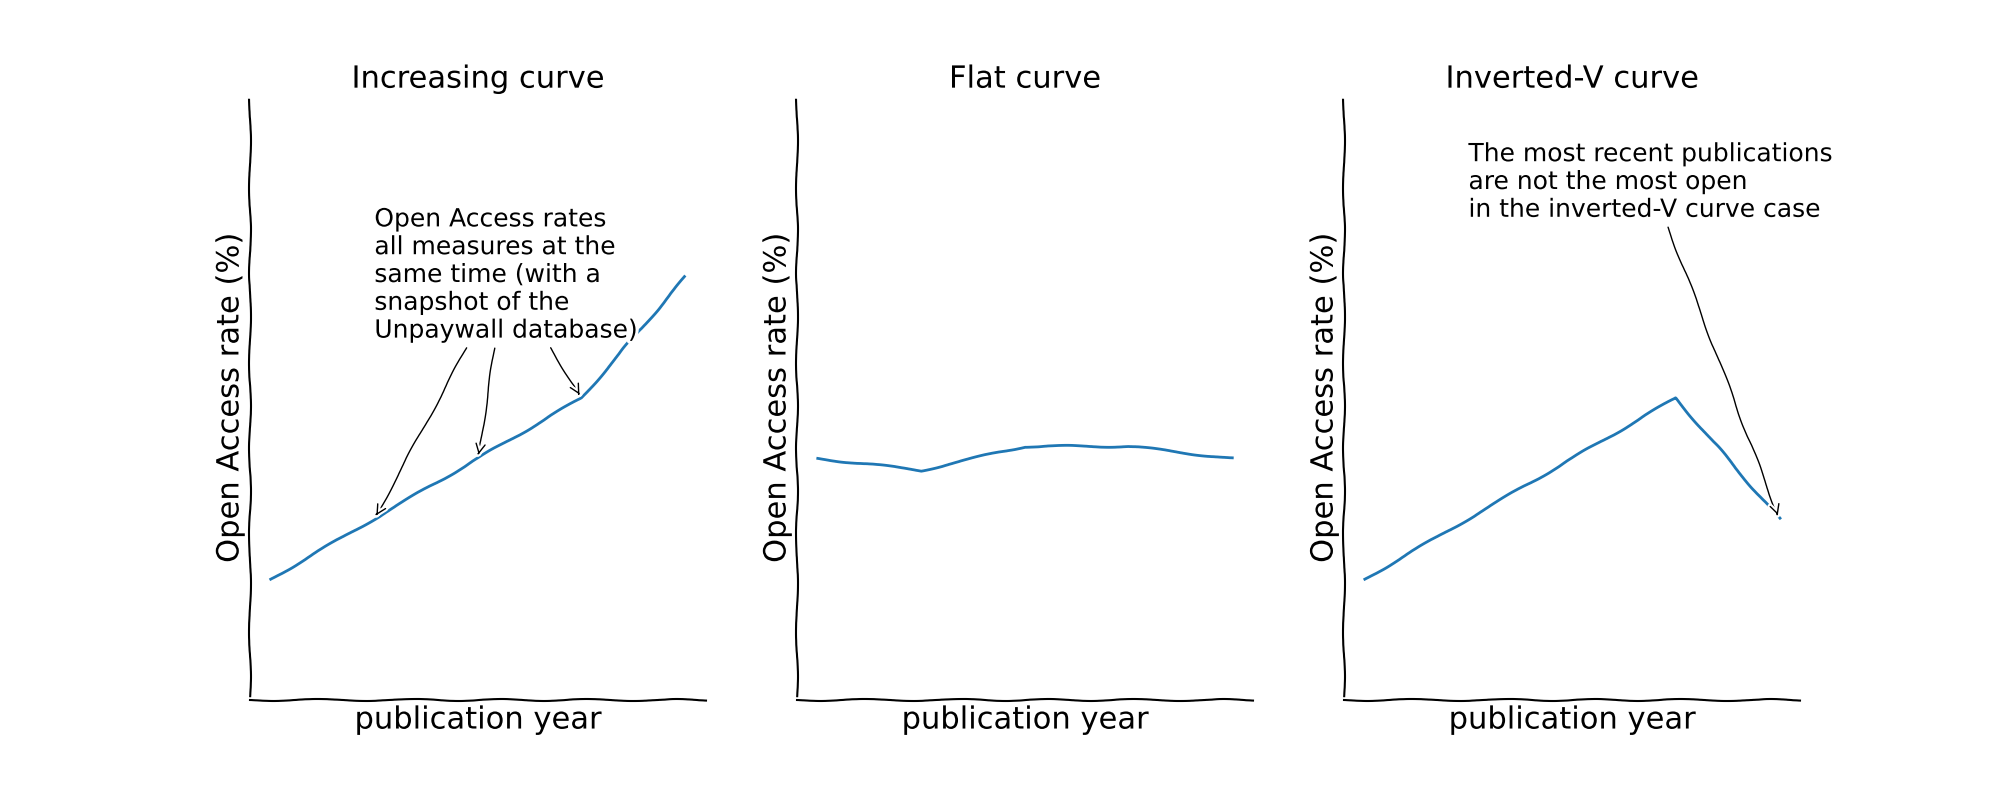
\includegraphics[width=6.25in,height=\textheight]{https://raw.githubusercontent.com/dataesr/bso-publications/main/doc/types_curve.png}
\caption{Different shapes of Open Access curves}
\end{figure}

From an observation date to another, the OA curve shape may change. This
evolution of the shape gives an insight on the opening speed evolution.
Indeed, moving from an inverted-V shape, where the most recent papers
are not the most open, to an increasing shape would be a strong evidence
of the opening acceleration. The figure 2 illustrates the evolution from
an inverted-V shape, to flat and then to an increasing OA curve shape.

\begin{figure}
\centering
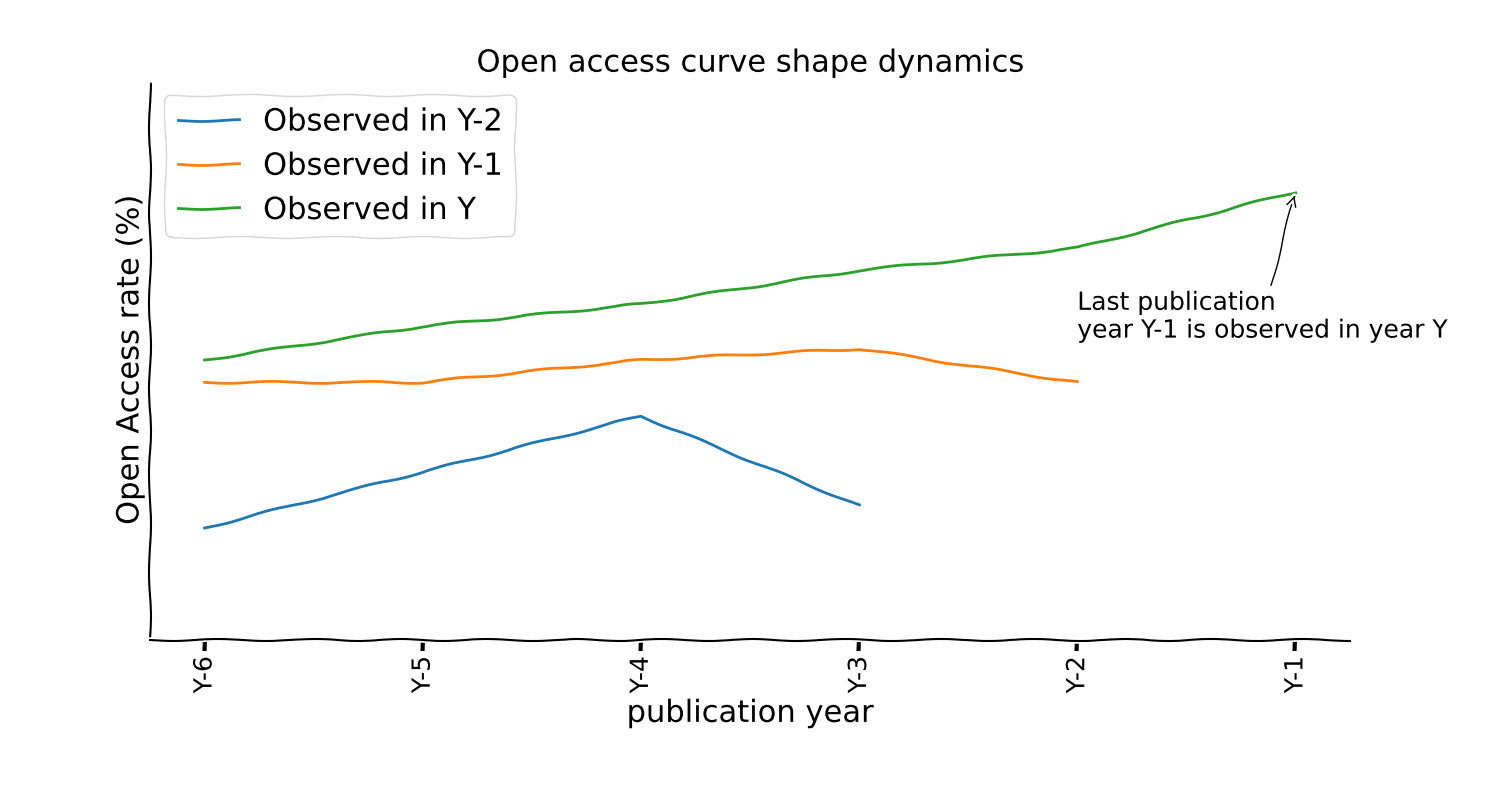
\includegraphics[width=6.25in,height=\textheight]{https://raw.githubusercontent.com/dataesr/bso-publications/main/doc/curve_dynamic.png}
\caption{Open Access curve dynamics}
\end{figure}

\hypertarget{open-access-types}{%
\subsubsection{2.1.3 Open access types}\label{open-access-types}}

As Unpaywall is the Open Access discovery tool we used, we initially
based our results on the OA classifications described in (Piwowar et al.
2018). It breaks down the OA types in 5 categories: `Gold', `Hybrid',
`Bronze', `Green', `Closed'. These categories are also present in the
Unpaywall database (and oaDOI API) in the field `oa\_status'. We first
simply regrouped the categories `Gold', `Hybrid' and `Bronze' under a
`Publisher hosted' label. However, we now propose another classification
that we think more appropriate, at least for the French OA policy
steering.

(Piwowar et al. 2018) defined `Green' as `Toll-access on the publisher
page, but there is a free copy in an OA repository'. That implies that a
publication that would be free to read on the publisher webpage and that
would, at the same time, have a free copy on a repository would not be
counted as `Green'. That derives from the idea that the Version of
Record (VoR), available on the publisher website, is the preferred OA
version of the publication (REF à ajouter). As a consequence, the
repositories contribution to OA is mechanically reduced in favor of the
publishers one. This therefore blurs the picture of the extension of
repositories impact. That led us to propose a first level of analysis,
with 3 categories (excluding `Closed'):

\begin{itemize}
\item
  \textbf{hosted only on an open repository}: Toll-access on the
  publisher page, but there is a free copy in an OA repository,
  corresponding exactly to the `Green' definition of (Piwowar et al.
  2018), that we could rather label `Green only'
\item
  \textbf{hosted only by the publisher}: Free to read on the publisher
  webpage, but no free copy in any OA repository harvested by Unpaywall.
\item
  \textbf{hosted on an open repository and by the publisher}: Free to
  read on the publisher webpage and there is a free copy in an OA
  repository.
\end{itemize}

Obviously, this does not impact the overall Open Access rate, but this
balanced division, with no preference for the VoR, gives a different
picture. It seems that a similar choice has been recently made to
represent COKI data and its sources of openness
\url{https://openknowledge.community/dashboards/coki-open-access-dashboard/}

The figure 3 shows the kind of impact choosing one or the other OA type
break down.

\begin{figure}
\centering
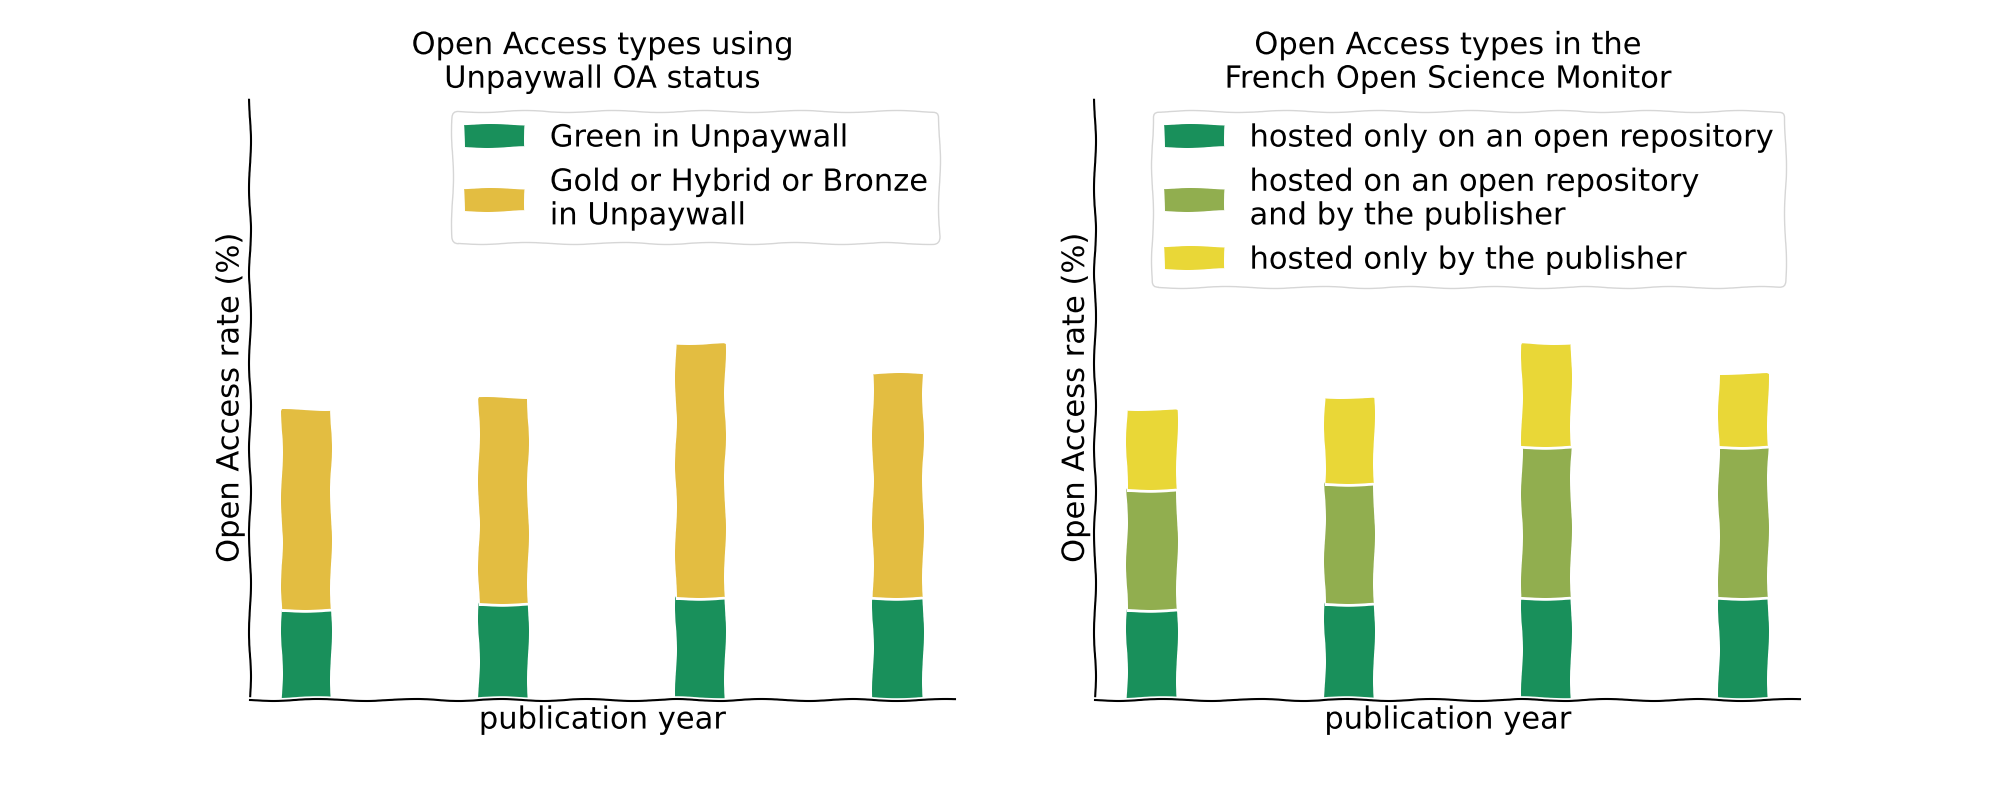
\includegraphics[width=6.25in,height=\textheight]{https://raw.githubusercontent.com/dataesr/bso-publications/main/doc/oa_types.png}
\caption{Open Access hosting types}
\end{figure}

\newpage

Another graphical way to represent this distribution is to use a bubble
chart (figure 4). Each bubble represents a cluster of publications (one
bubble is the equivalent for each discipline, for each dissemination
platform \ldots), its size depends on the number of publications in the
cluster. The x-axis represents the share of OA publications hosted by
the publisher, corresponding to the sum of publisher-only and publisher
/ open repository hosted publications. Conversely, the y-axis represents
the share of OA publications hosted on a repository, corresponding to
the sum of open repository-only and open repository / publisher hosted
publications.

\begin{figure}
\centering
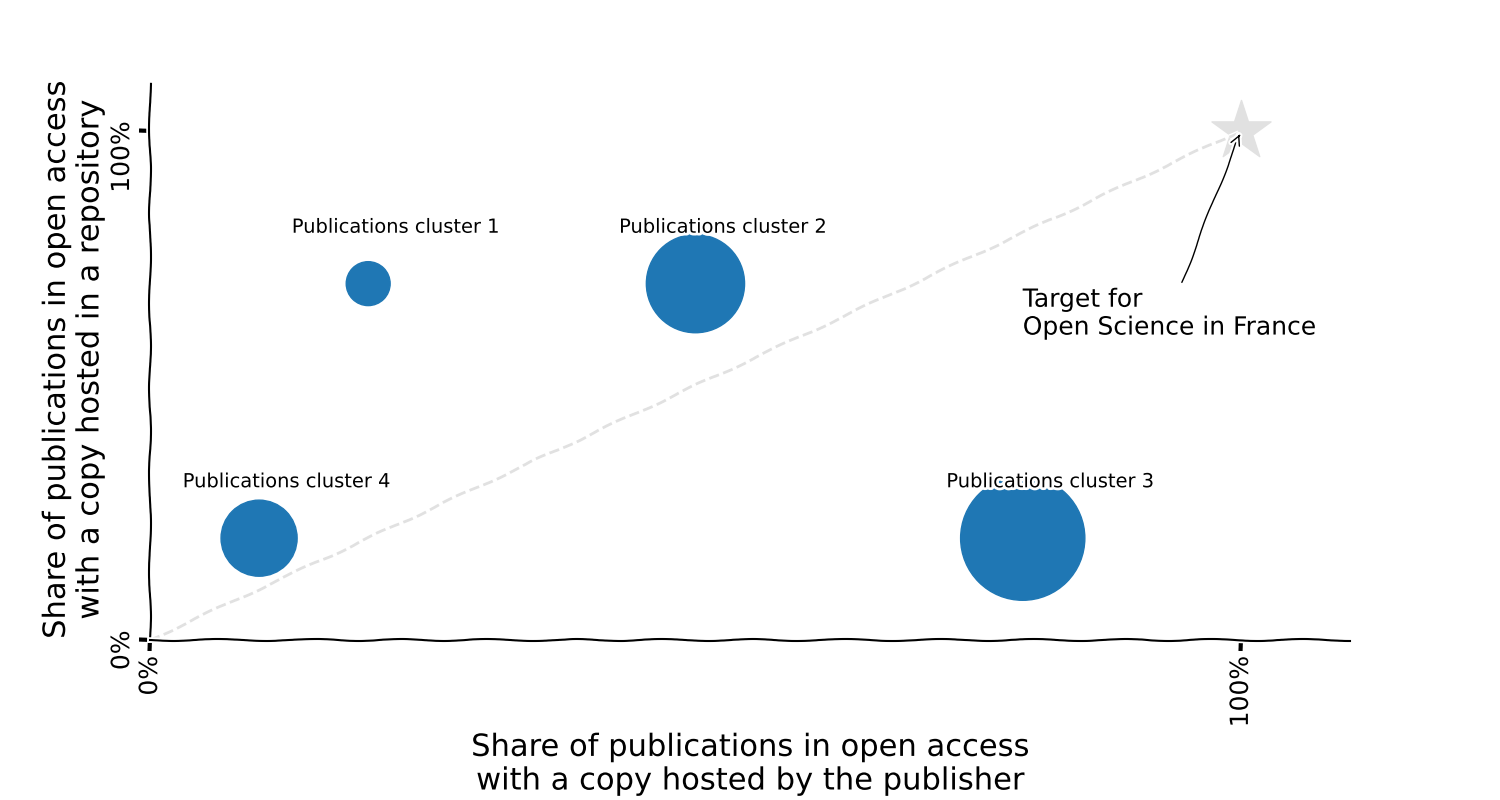
\includegraphics[width=6.25in,height=\textheight]{https://raw.githubusercontent.com/dataesr/bso-publications/main/doc/bubbles.png}
\caption{Share of publications in open access hosted on an open
repository vs.~by the publisher}
\end{figure}

The source of data used to compute these OA types is still Unpaywall,
but instead of the `oa\_status' field, we then use the `oa\_locations'
field. For a publication which is in open access, it lists all the
existing available copies that Unpaywall detected, at the time of the
snapshot. Each location is described, in particular with an URL that
gives a link to the given copy, and some metadata for the location is
associated, in particular the `host\_type', that take two possibles
values, `publisher' or `repository'. It is important to note that, for
now, preprint servers are always considered as repositories.

\hypertarget{discipline-and-language-impact}{%
\subsubsection{2.1.4 Discipline and language
impact}\label{discipline-and-language-impact}}

All disciplines and publication languages are covered, while no metadata
exists to describe the discipline or the publication language. To enrich
the metadata, we then rely on machine learning approches, that infer
discipline and language from the available metadata.

For the language detection, only the title and abstract are used if
available, with the lid.176.bin Fasttext word embedding machine learning
algorithm (Joulin et al. 2016).

Discipline detection also uses journal and keywords metadata if
available. A general classifier is implemented for all domains, which
classifies the publications into 10 macro disciplines: Mathematics,
Chemistry, Physics \& astronomy, Fondamental biology, Medical research,
Computer sciences, Earth science ecology energy \& applied biology,
Humanities, Social sciences, Engineering. It is trained on data from the
Pascal \& Francis database and uses a Fasttext classifier. More details
are discussed in the previous paper (Jeangirard 2019).

A domain-specific classifier is implemented for the Health domain. It
classifies the publications into 17 disciplines, built from the Fields
of Research taxonomy. The full methodology is detailed in (Jeangirard
2021).

The main purpose of these metadata enhancements is to be able to analyse
the open access rate according to languages and disciplines. We expect
to observe differences not only in the global OA rate (Which discipline
is the most open?), but also in the dynamics trends (Which discipline
shows the strongest increase over time?) or in the opening practices
(relying on publisher hosted open access versus open repositories).

\hypertarget{publishers-and-dissemination-platforms-strategies}{%
\subsubsection{2.1.5 Publishers and dissemination platforms
strategies}\label{publishers-and-dissemination-platforms-strategies}}

\hypertarget{identification-of-the-dissemination-platforms}{%
\paragraph{2.1.5.1 Identification of the dissemination
platforms}\label{identification-of-the-dissemination-platforms}}

The data in the `publisher' field of Crossref shows many
inconsistencies. There are many journals, with a single ISSN, that
belong to more than one publisher - whether they are different lexical
forms or refer to actual different entities. Consequently, we performed
a triple grouping in order to facilitate the coding of an economic
entity disseminating the journal in question.

\begin{itemize}
\item
  Firstly, we have considered the diversity of lexical forms of the same
  publisher, existing in developed form and in the form of acronyms,
  including or not its economic status (LLC, Ltd.,\ldots);
\item
  Secondly, we have taken into account the capitalist evolution of the
  sector, which is marked by a growing concentration, with successive
  takeovers (Larivière, Haustein, and Mongeon 2015). The latter do not
  necessarily make the old group names vanish, as they are often used as
  a brand name of the new entity(e.g.~Palgrave being a brand of the
  Springer Nature group);
\item
  Thirdly, we have taken into account the possible distinction between
  publisher and dissemination platform, with many scholarly societies
  remaining the owner and publisher, but delegating the dissemination of
  their publications to a given publisher/disseminator though multi-year
  contracts.
\end{itemize}

We historicized the last two groupings to account for the effective date
of the link between these different entities. All coding is available in
the open source code hosted at
\url{https://github.com/dataesr/bso-publications/tree/main/bso/server/main/publisher}.

\hypertarget{business-models-and-open-licences}{%
\paragraph{2.1.5.2 Business models and open
licences}\label{business-models-and-open-licences}}

As explained above, the `oa\_status' in Unpaywall data belittles the
role of open repositories. It also invisibilize Diamond open access,
indifferently mixing in the same `Gold' category all publications in an
open-access journal that is indexed by the DOAJ, whether Article Process
Charges (APC) are part of the business model or not. That is why we
introduce another level analysis, about the dissemination platform
business model, with 3 categories :

\begin{itemize}
\item
  \textbf{Diamond}: articles published in an open-access journal indexed
  by the DOAJ, and without APC (according to the DOAJ data). This
  category may be under-estimated as many journals have a no-APC model
  are not currently included in the DOAJ (Bosman et al. (2021))
\item
  \textbf{(Full APC) Gold}: articles published in an open-access journal
  (using the field `journal\_is\_oa' = True from Unpaywall) and with an
  estimated APC, as described above.
\item
  \textbf{Hybrid}: publications published in a journal that is not full
  open access (using the field `journal\_is\_oa' = False from Unpaywall)
  and with an estimated APC, as described above.
\item
  \textbf{Other}: all other cases, in particular publications with
  moving barriers, but also cases for which no information about APC has
  been collected. This category may be over-estimated as some journal
  have no APC but this information is not present in a structured
  database.
\end{itemize}

The objective of this level of analysis is to separate different
business models (APC vs Diamond vs Hybrid), not to analyze the open
licences associated to the OA copies, so this categorization is quite
different from the Gold / Hybrid / Bronze from (Piwowar et al. 2018).

For that matter, a third analysis level is used that distinguishes, for
open access publications:

\begin{itemize}
\item
  \textbf{Creative commons} licences (cc0, cc-by, cc-by-nc etc \ldots)
\item
  \textbf{Other licences} (publisher specific, country-specific \ldots)
\item
  \textbf{No licence}
\end{itemize}

To be clear, the no licence category does not mean that the publications
are closed, on the contrary they are in freely available but no open
licence was detected, meaning the reuse conditions, beyond reading, are
not defined. They are certainly not BOAI-compliant (REF), but considered
as ``open'' in our context.

Again, the informations from the field `oa\_locations' comes from
Unpaywall, therefore the results depend on the quality of the Unpaywall
database.

\hypertarget{article-processing-charges-apc-estimation}{%
\paragraph{2.1.5.3 Article Processing Charges (APC)
estimation}\label{article-processing-charges-apc-estimation}}

Estimating APC for each journal article remains difficult as few open
sources exist. We leverage on the openAPC database (at the publication
level) and on the DOAJ data (at the ISSN level). We use the following
heuristics to estimate the APC of a publication :

\begin{itemize}
\item
  If the DOI is not in open access with a free copy on the publisher
  webpage, there is no APC estimation to make.
\item
  Else, if the DOAJ specifies there are no APC for the ISSN, then it is
  a Diamond DOAJ OA, with no APC.
\item
  Else, if the DOI is explicitly in the openAPC database, we simply use
  the APC from openAPC.
\item
  Else, if the DOI is not in the openAPC database, but its ISSN or
  publisher is, with a sufficient number of observations, we use the
  mean of the APC observed for the same ISSN or the same publisher,
  during the same year if enough data is available, or over the whole
  openAPC database otherwise.
\item
  Else, if the DOAJ specifies there are APC for the ISSN, we simply use
  the APC from DOAJ, after a conversion to Euros if needed (based on the
  exchange rate at the publication date).
\item
  Otherwise, no estimation is made.
\end{itemize}

We are aware that this estimation is far from being perfect, but it
still brings some insights. On top of that, even if we focus on French
publications (publications with at least one author with a French
affiliation), the sum of the APC estimated is higher than the actual
amount of APC money spent by French institutions, as a large share of
the publications are co-authored with scholars affiliated to foreign
institutions. Informations on the corresponding author could be a proxy
to focus on APC spent by France but for now, we do not have an open,
reliable and massive source for this information.

\hypertarget{the-role-of-the-open-repositories}{%
\subsubsection{2.1.6 The role of the open
repositories}\label{the-role-of-the-open-repositories}}

\hypertarget{other-analysis-axes}{%
\subsubsection{2.1.7 Other analysis axes}\label{other-analysis-axes}}

In the case of the Health domain, we use metadata coming from PubMed.
These metadata are quite rich and enable extra analysis. In particular,
some \textbf{funding metadata} are present in PubMed, as well as the
\textbf{affiliations for each author} (it is far from being the case
when using other sources and scrapped metadata).

PubMed gives information on grant declaration. To be clear, the absence
of this metadata does not mean that there was no specific funding
leading to the given publication. So the only thing we are able to do is
to check whether a correlation exist between the open access rate and
the presence of the grant metadata in PubMed.

As the affiliations information is given for each author, we can use
(L'Hôte and Jeangirard 2021) to infer the country of affiliations of
each author. We wish to analyze whether the country of affiliation of
the corresponding author correlates to the open access rate or not.
Unfortunately, the corresponding author metadata is not available, that
is why we chose an approximation looking at the affiliation country of
the \textbf{first and the last authors}. That will give an insight to
know whether, for French publications, the OA rate is in general higher
when one of the first or last authors has a French affiliation, or,
conversely, if the OA rate is higher when the first and last author are
affiliated abroad.

\hypertarget{clinical-trials-and-observational-studies}{%
\subsection{2.2 Clinical trials and observational
studies}\label{clinical-trials-and-observational-studies}}

The French Open Science Monitor focused only on publications. Current
work is being conducted on monitoring Research Data and Software Code.
The French Open Science Monitor in Health, however, already introduces
new research objects specific to the Health domains: clinical trials and
observational studies.

In the USA, reporting and publication of results is mandatory for all
clinical trials. The reporting registry used is
https://clinicaltrials.gov/. This website is also used by many
international actors. It also welcomes reports of observational studies,
though this reporting is not mandatory.

In European Union countries, the reporting obligation will only extend
to clinical drugs from 2022 on. The European registry
https://www.clinicaltrialsregister.eu/ (EUCTR) therefore mainly includes
clinical trials involving medicines, and less frequently observational
studies, clinical trials involving surgical protocols, medical devices
or psychotherapeutic protocols.

The issue of opening up or sharing data arises for clinical research in
the same way as for other areas of scientific research. However, it has
a particularly complex dimension, since it involves personal data, some
of which directly concern the health of individuals. Nevertheless, it is
possible to define the modalities for sharing this data.

Two dimensions will be developed:

\begin{itemize}
\item
  The openness of the results and publications when the study is
  completed.
\item
  The declaration of clinical and observational studies in these public
  registries.
\end{itemize}

\hypertarget{perimeter}{%
\subsubsection{2.2.1 Perimeter}\label{perimeter}}

For now, two datasources are used to collect metadata about clinical
trials and observational studies: clinicaltrials.gov and EUCTR. The
former one provides an API while the latter one does not; that is why
the information is crawled from the website. Only the trials and studies
that involves at least \textbf{one location in France} are analyzed.

Some trials or studies appear in both registries, the matching between
the two databases being done based on the PIDs NCTId (from
clinicaltrials.gov) and eudraCT (from EUCTR), both registries keeping
track of external PIDs. However, duplicates may still remain when no
link has been established between the existing PIDs in both registries.

To distinguish clinical trials on one side and observational studies on
the other, we use the study type field, that can be either
`Interventional' (for clinical studies) or `Observational' (for
observational studies).

\hypertarget{main-opening-indicators}{%
\subsubsection{2.2.1 Main opening
indicators}\label{main-opening-indicators}}

Two key types of indicators are analyzed:

\begin{itemize}
\tightlist
\item
  The declaration of results and / or scholarly publications after a
  trial or study is completed. (Goldacre et al. 2018) showed that a
  large fraction of trials do not report their results in the databases
  or publications. On top of the results declaration rate itself, we
  look into the results' date of registration, assessing the delay
  between the end of the trial and the actual reported results date.
\end{itemize}

We propose both indicators, mixing or separating results and scholarly
publications. For publications, it is important to note that only the
metadata from the studies registries are used, without trying to link
trials to DOIs using the publications metadata (with PubMed for
example). The open access status of these publications is also retrieved
from the Unpaywall data.

\begin{itemize}
\tightlist
\item
  The delay to register the study: is the trial or study publicly
  registered before it actually starts, or is it done afterwards ? And
  how many months is the actual delay to register ? Does it evolves over
  time ?
\end{itemize}

\hypertarget{lead-sponsor-impact}{%
\subsubsection{2.2.2 Lead sponsor impact}\label{lead-sponsor-impact}}

(Goldacre et al. 2018) gives evidence that the rate of results
declaration is very impacted by the type of lead sponsor, commercial
sponsors having a much higher declaration rate. We therefore propose to
break down most of the analysis axis with the type of lead sponsor,
being either academic or industrial. This categorization has been done
manually based on the lead sponsor name.

\hypertarget{local-open-science-monitors}{%
\subsection{2.3 `Local' Open Science
Monitors}\label{local-open-science-monitors}}

The University of Lorraine was the first institution to provide a local
version of the French Monitor (Bracco 2022):
\url{https://scienceouverte.univ-lorraine.fr/barometre-lorrain-de-la-science-ouverte}.

This local version, published during spring 2020, was designed with
reusability in mind. For this purpose, the code has been detailed step
by step in Jupyter Notebooks and includes a readme file explaining all
the required actions to obtain its own Monitor.

The code created on this occasion is freely accessible (Bracco 2020).

The availability of the code was combined with numerous training
sessions as well as individual assistance provided by the University of
Lorraine to each institution that requested it.

Following the publication of this code, many institutions were able to
generate their own Open Science indicators. This enthusiasm for local
implementation has underlined the need for institutions to have reliable
and effective tools for monitoring Open Science.

The new version of the national Monitor enables, directly from the
website, to generate graphs from a list of DOIs previously sent to the
French Ministry of Higher Education, Research and Innovation team. The
University of Lorraine has been asked to test and implement this new
version.

The constitution of the DOI corpus remains an essential step for
institutions. The code proposed by the University of Lorraine makes it
possible to generate this list simply by crossing various databases.

This simplified version will probably encourage other institutions to
establish their own Monitor.

\hypertarget{data-collection-system-and-architecture}{%
\subsection{2.4 Data collection system and
architecture}\label{data-collection-system-and-architecture}}

In this section, we will try to present the global workflow to collect,
enrich and consolidate the data as described before with the technical
and the storage challenges.

We collect data from multiple sources (PubMed, Crossref, parsed html
\ldots), and then try to determine the affiliations' countries. From the
Crossref DOIs, we collect more details about that publication via
Unpaywall (title, published year, ISSNs, but also open access locations
if any).

Each step consumes time and CPU. Assuming any step can fail at any time,
we choose to develop each step as independent and idempotent.

From the different datasources, we store the raw data on Object Storage
on the public OVH Cloud. These data are then transformed into a common
`pivot' json schema, and enriched with affiliations countries, so that
only the French publications are kept in the rest of the process. These
publications metadata are then enriched with Unpaywall informations
(open access locations), openAPC and DOAJ informations to infer if APC
were paid or not.

Eventually, the data is loaded in an elasticsearch cluster that is
consumed by the French Open Science Monitor User Interface.

\begin{figure}
\centering
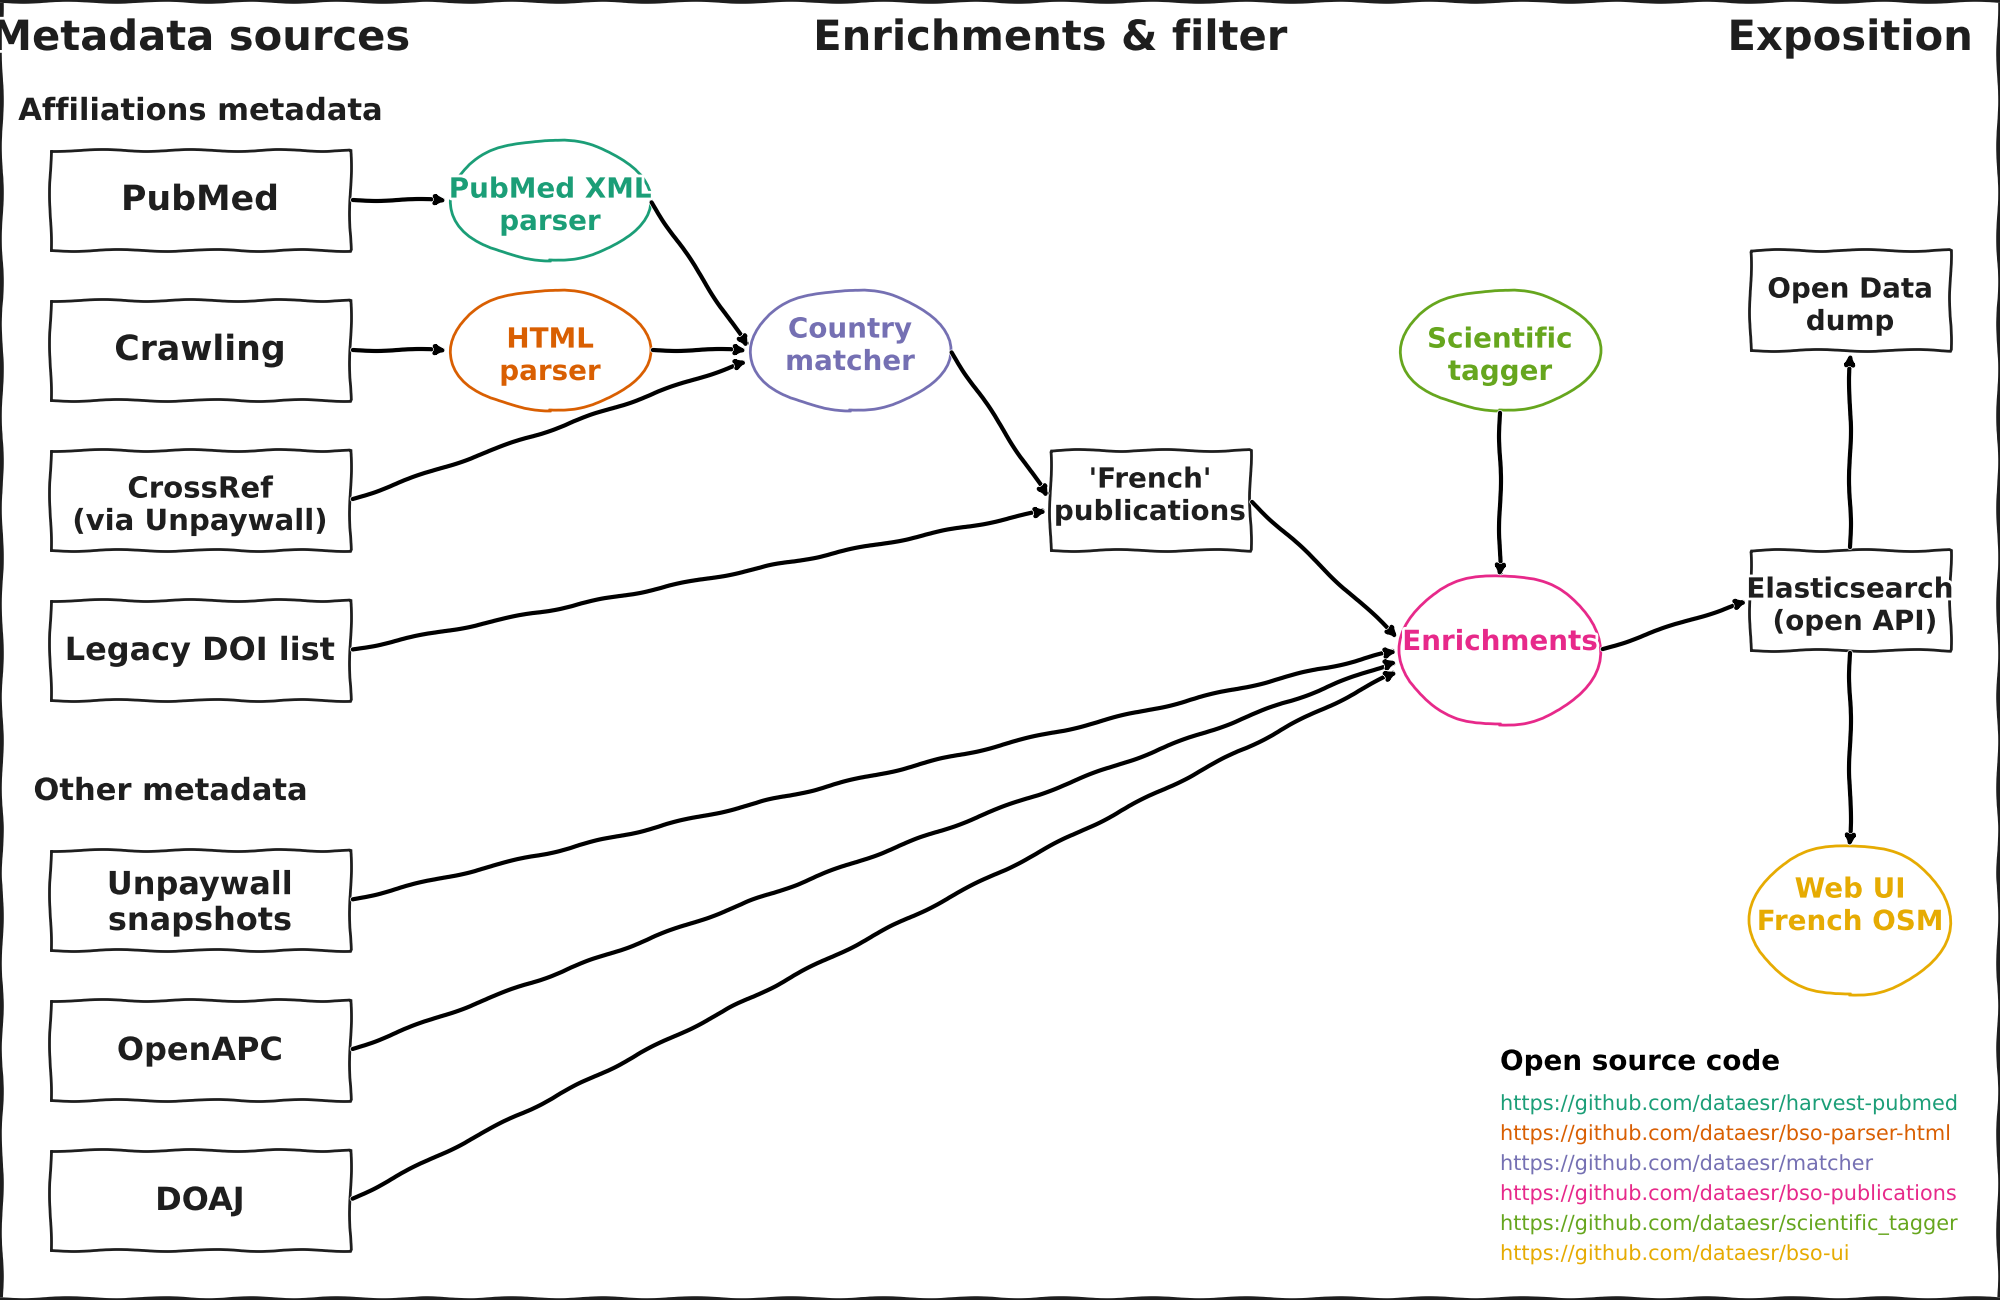
\includegraphics[width=6.25in,height=\textheight]{https://raw.githubusercontent.com/dataesr/bso-publications/main/doc/flow_chart_publications.png}
\caption{Global overview of the publications data flows}
\end{figure}

A similar workflow, yet simpler is set up for clinical trials.

\begin{figure}
\centering
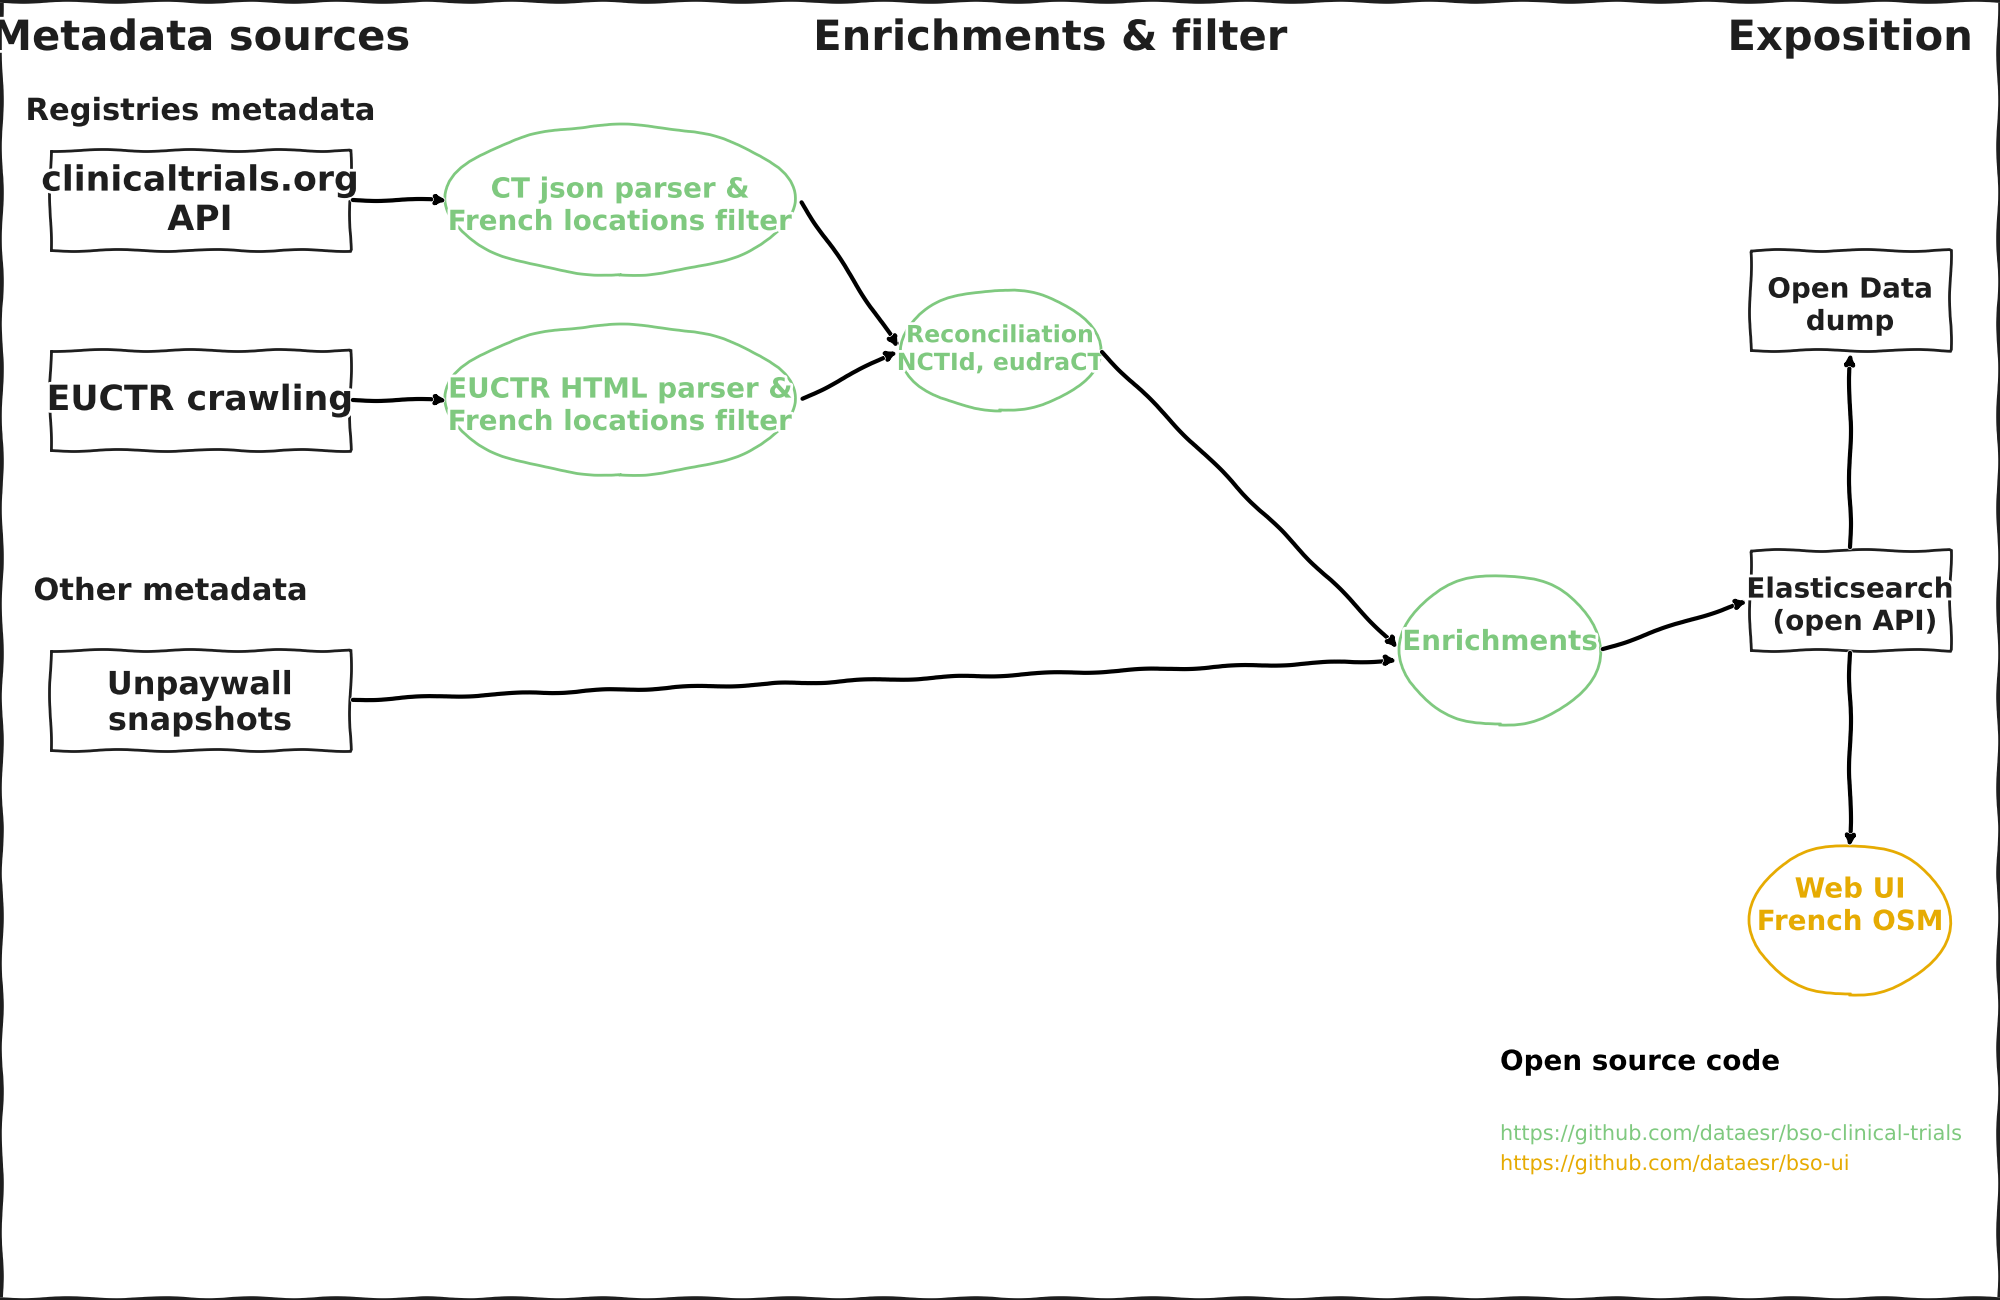
\includegraphics[width=6.25in,height=\textheight]{https://raw.githubusercontent.com/dataesr/bso-publications/main/doc/flow_chart_registries.png}
\caption{Global overview of the trials and studies data flows}
\end{figure}

\hypertarget{results}{%
\section{3. Results}\label{results}}

The results are extracted from the French Open Science Monitor website
https://frenchopensciencemonitor.esr.gouv.fr from February 2022.

\hypertarget{open-access-dynamics-in-france}{%
\subsection{3.1 Open access dynamics in
France}\label{open-access-dynamics-in-france}}

\hypertarget{general-dynamics}{%
\subsubsection{3.1.1 General dynamics}\label{general-dynamics}}

The steady increase in the open access rate observed each year since
2018 is an indicator of the impact of public policies in favour of open
access. It is a proof of the evolution of researchers' publication
practices, the strengthening of open access publication infrastructures
and the strategies of scientific publishing actors. Open access to
publications is an evolutionary process over time. A publication that is
not available in open access at the time of its publication may become
so in the following months and years, through various mechanisms:
deposit by the author in an open archive after a period of embargo
imposed by the publisher or the application by the publisher of a moving
barrier, i.e., a time limit at the end of which it itself makes the
publication available in open access.

The figure 7 presents, for each observation date since 2018, the open
access rate of French scientific publications published during the
previous year. The observations made during the current year are updated
every quarter. Thus, 52\% of French scientific publications published in
2019 were in open access in 2020 (observation date). And 62\% of French
scientific publications published in 2020 were open in 2021. The access
rate has thus increased by 10 points in just one year.

\begin{figure}
\centering
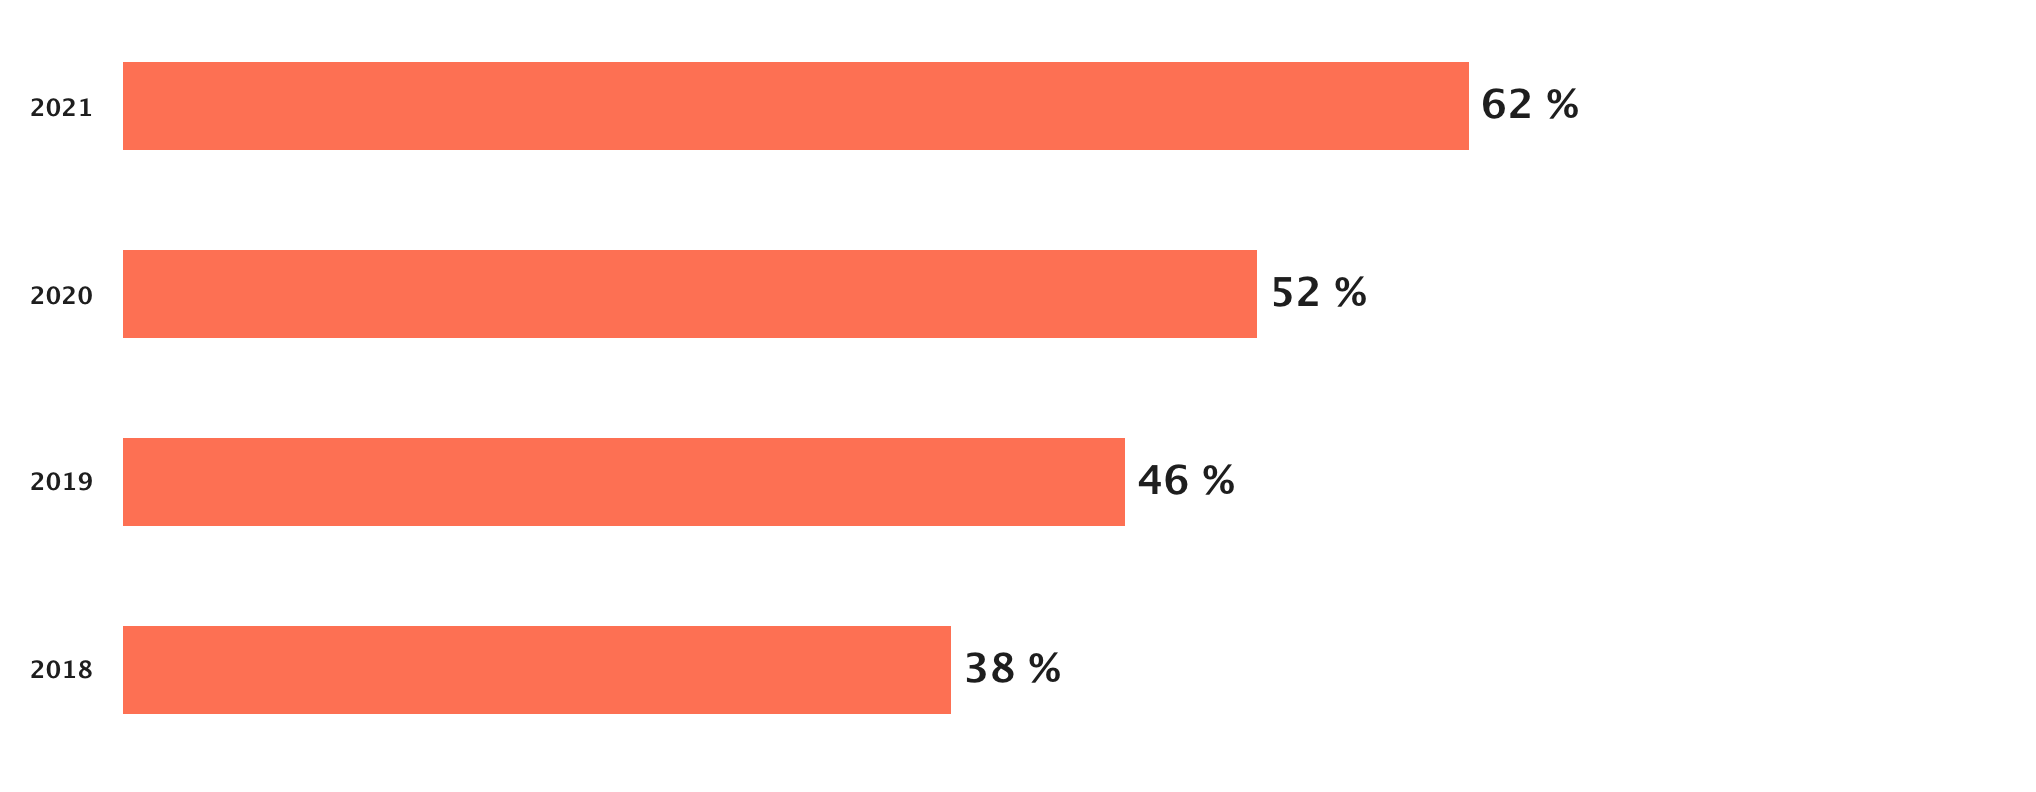
\includegraphics[width=6.25in,height=\textheight]{https://raw.githubusercontent.com/dataesr/bso-publications/main/doc/results_publications_1.png}
\caption{Open access rate of scientific publications in France published
during the previous year by observation date}
\end{figure}

The figure 8 presents, for each observation date, the open access rate
of scientific publications in France by publication date. Each line
represents the open access rates observed for an observation date, and
the open access rates are expressed as a function of the publication
year. For each year of publication, it is observed that the open access
rate increases according to the date of observation. This is due to the
process of releasing the most recent publications through the expiry of
moving barriers or deposits on open archives after an embargo period. As
a result, the open access rate of publications released in 2017 has
increased from 38\% in 2018 to 51\% in 2021. When the open access rate
is higher in the latest year of publication than in previous years, this
is an indication of a shortening of the timeframe for open access
provision.

\begin{figure}
\centering
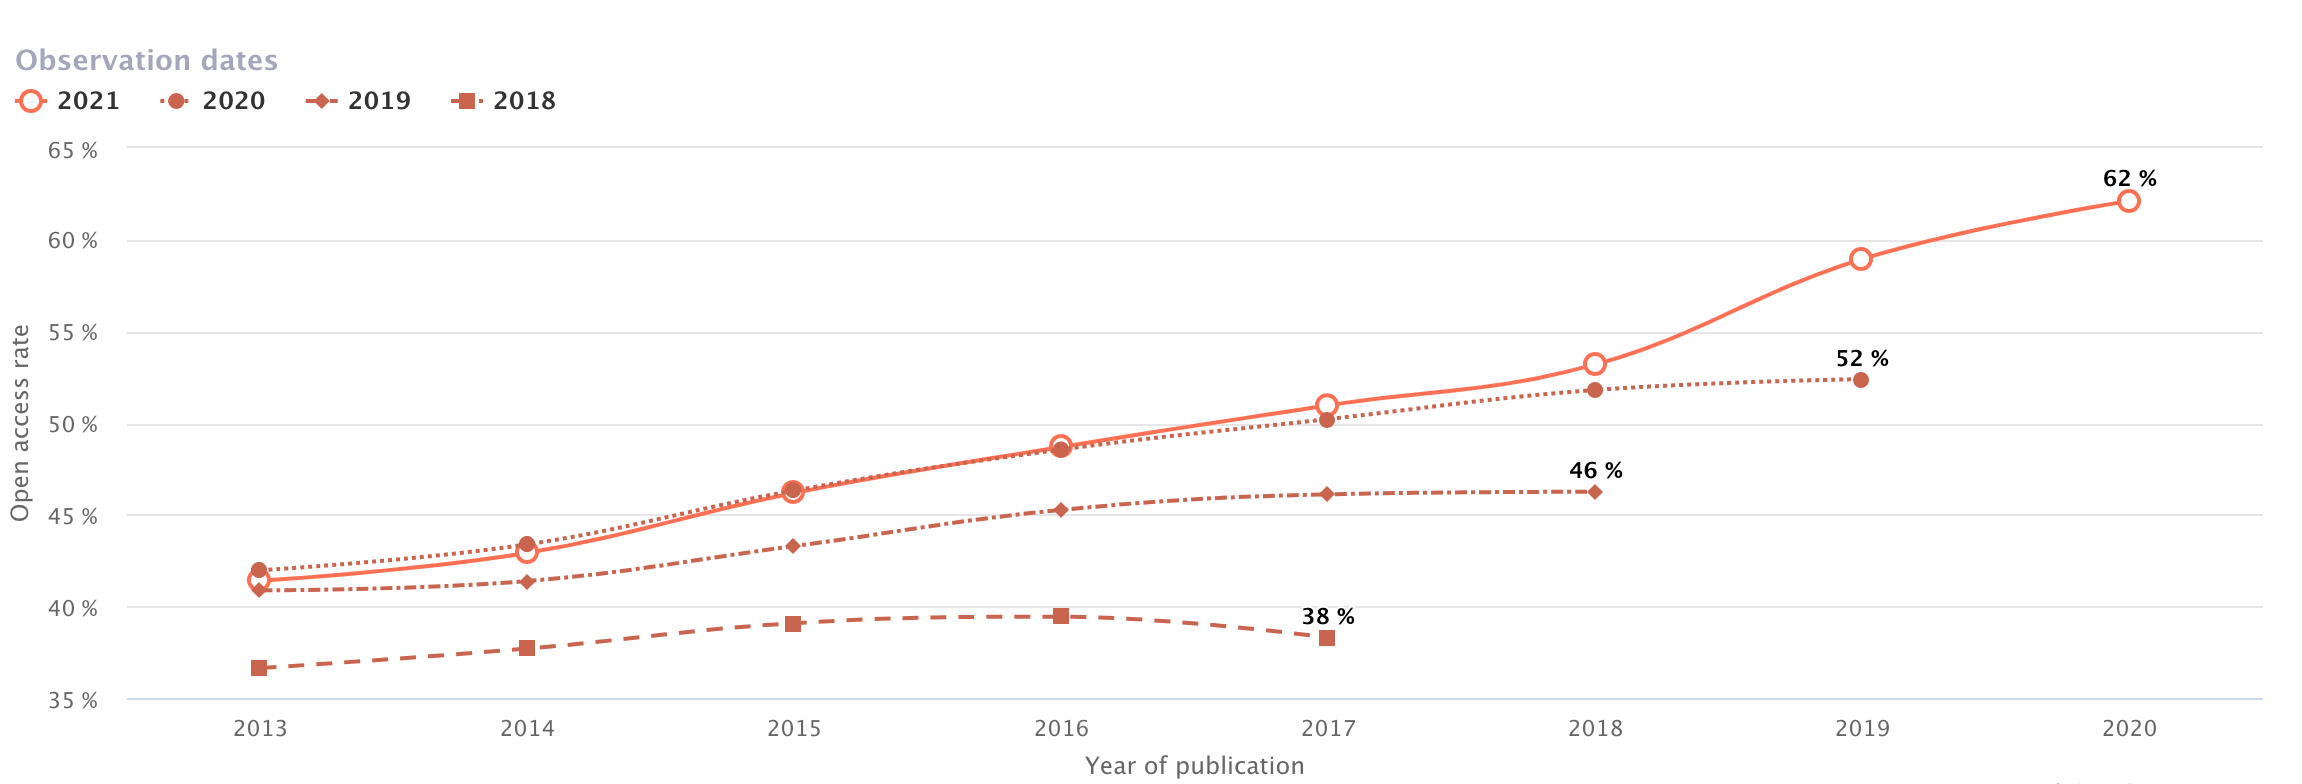
\includegraphics[width=6.25in,height=\textheight]{https://raw.githubusercontent.com/dataesr/bso-publications/main/doc/results_publications_2.png}
\caption{Evolution of the open access rate of scientific publications in
France by year of observation}
\end{figure}

Open access to scientific publications can be achieved through several
routes: natively open access publication by the publisher on a
dissemination platform or deposit by the author in an open repository.
These two routes are not exclusive, as a publication may be available
both on an open repository and on the publisher's publishing platform.
This simultaneity, which tends to increase over time, is a factor of
resilience since it makes it possible to offer editorial quality and
guarantee the durability of access to French scientific publications. We
observe that, for publications published in 2020, 28\% are open via both
routes, 18\% only via an open repository and 16\% only via the publisher
(figure 9).

\begin{figure}
\centering
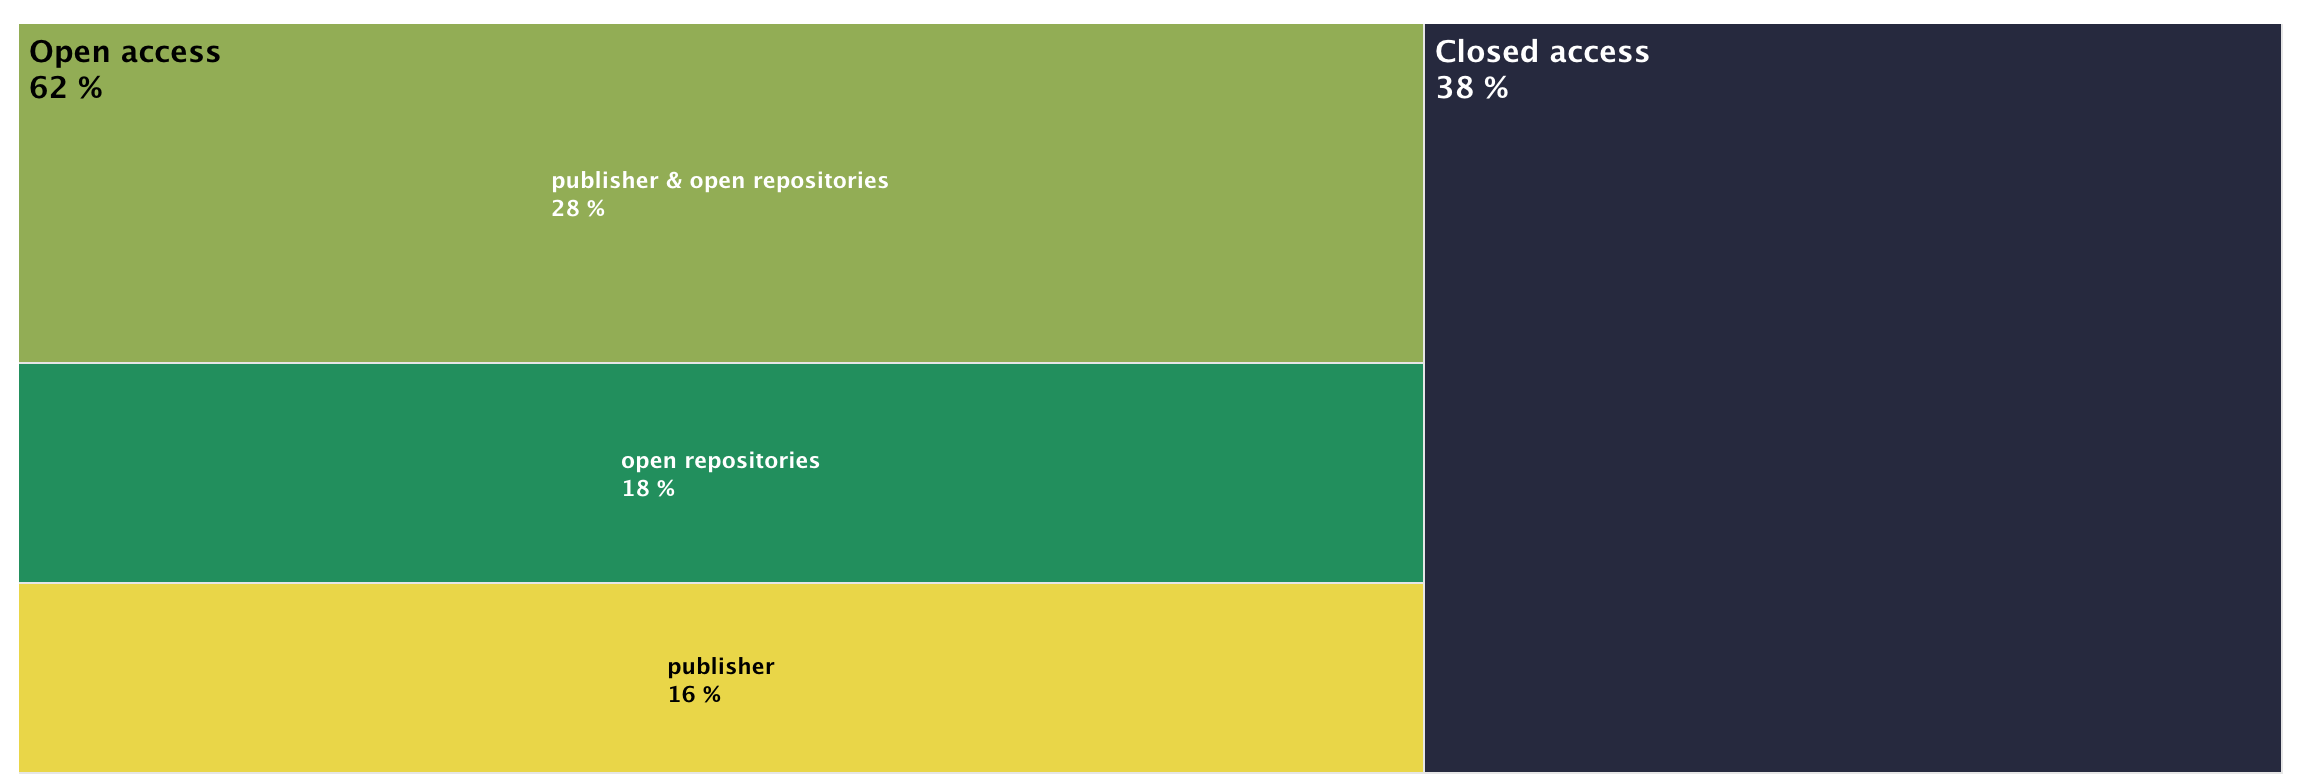
\includegraphics[width=6.25in,height=\textheight]{https://raw.githubusercontent.com/dataesr/bso-publications/main/doc/results_publications_3.png}
\caption{Distribution of scientific publications in France published in
2020 by opening route (observed in 2021)}
\end{figure}

The figure 10 shows, for the most recent observation date (2021), how
open access publications in France issued in the previous year are
distributed by opening route.

\begin{figure}
\centering
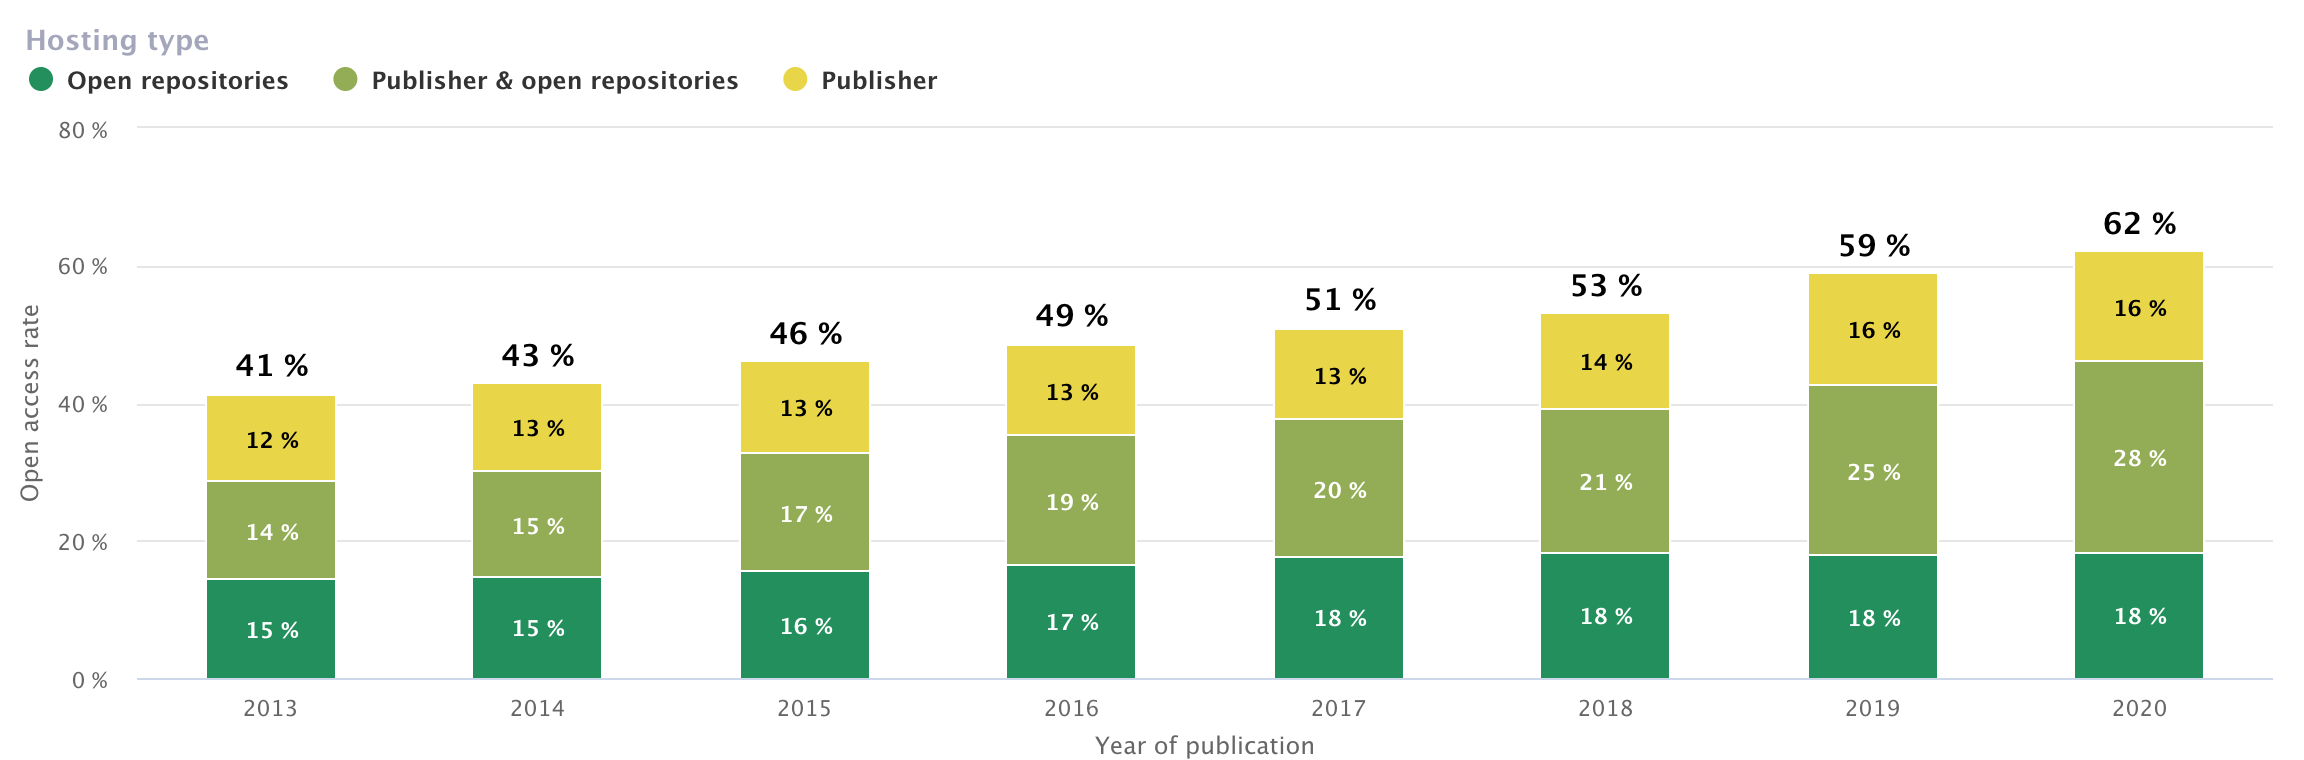
\includegraphics[width=6.25in,height=\textheight]{https://raw.githubusercontent.com/dataesr/bso-publications/main/doc/results_publications_4.png}
\caption{Distribution of the open access rate of publications in France
per publication year and by OA route (observed in 2021)}
\end{figure}

Scientific publications take a variety of forms: articles are the most
common, but there are also books (monographs written by a single author
or collective works bringing together various contributions), conference
proceedings, preprints, i.e.~articles proposed for discussion before
submission to a scientific journal, etc. The preferred types of
publication differs according to disciplines and disciplinary
communities. Each type of publication has its own dissemination logic,
which explains why open access rates vary from one to another. In
particular, we note that the monitor measures a ratio of 65\% open
access for journal articles, and 30\% open access for book chapters
(figure 11). Open access initiatives have historically started with
journals and articles. Books and chapters are less involved in the open
access process, at least for their Crossref DOI part.

\begin{figure}
\centering
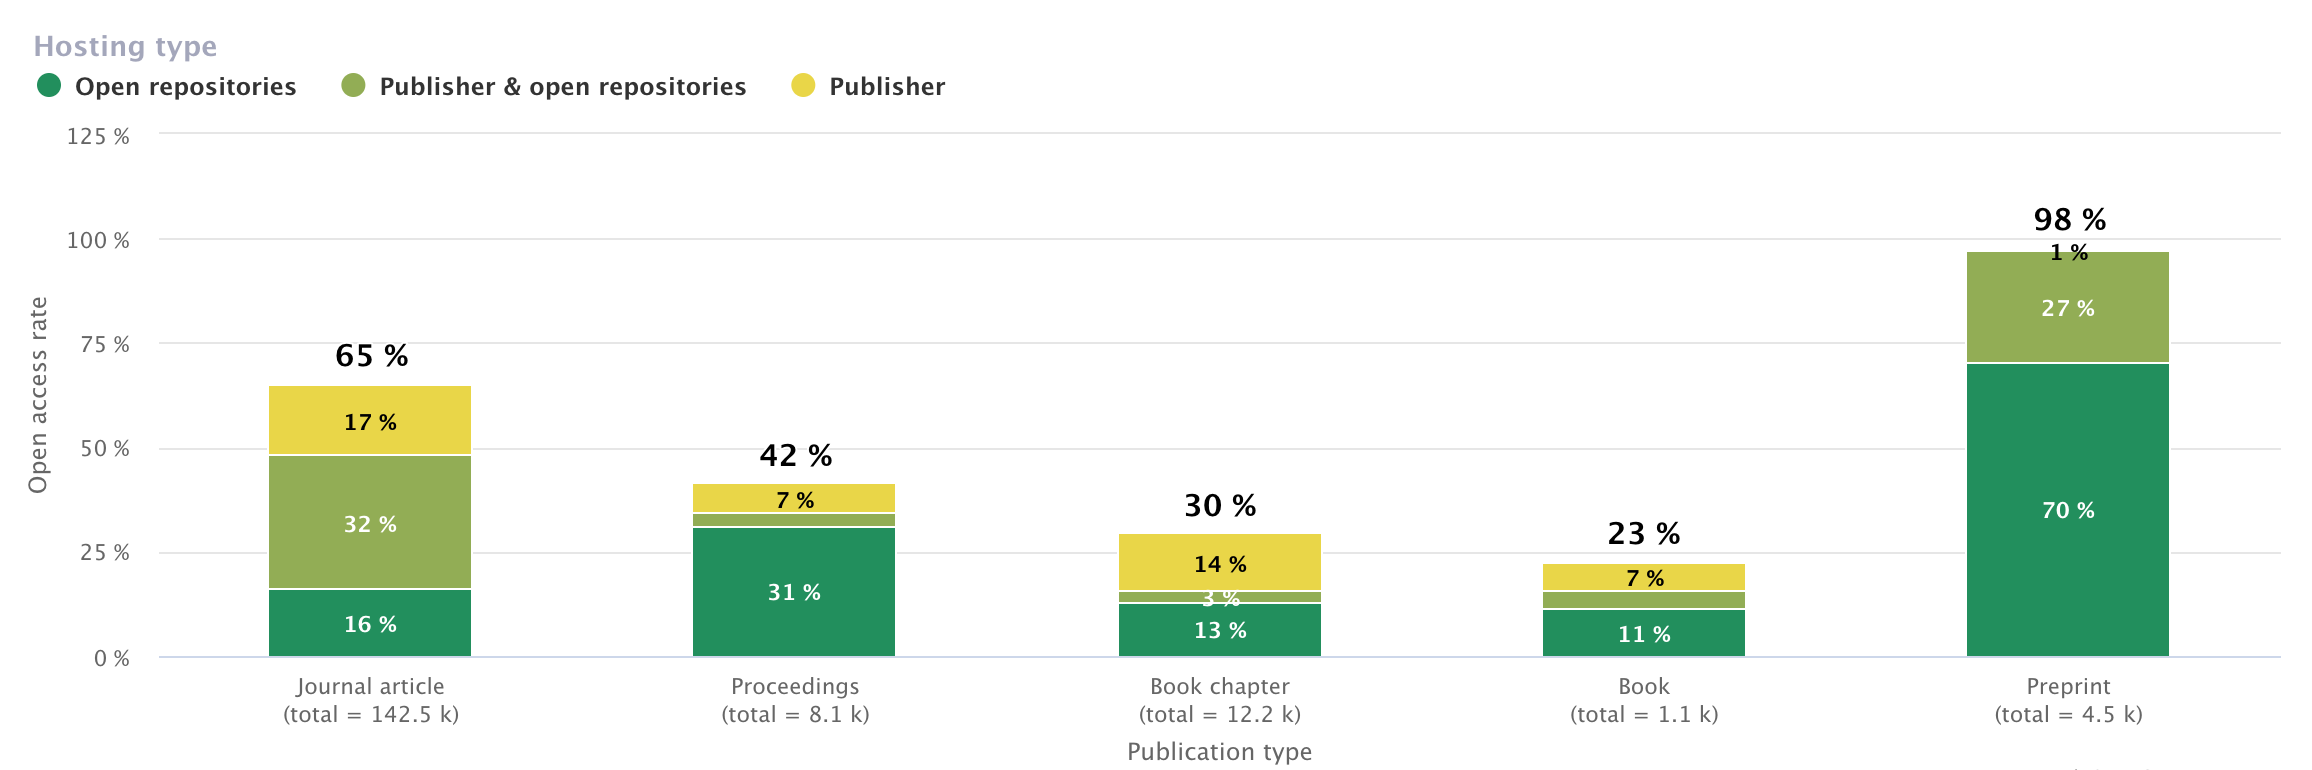
\includegraphics[width=6.25in,height=\textheight]{https://raw.githubusercontent.com/dataesr/bso-publications/main/doc/results_publications_5.png}
\caption{Open access rate by type of publications in France
(publications from 2020)}
\end{figure}

The monitor makes it possible to measure both the domination of English
as a scientific language and the significant maintenance of production
in French, which contributes to the multilingualism of scholarly
communication. Several factors must be taken into account in order to
interpret the difference in the rate of open access according to the
languages in which French researchers publish: international standards
in terms of open access, the specific practices of disciplines that
publish mainly in French or English, and the development of open access
publishing capacities in the various linguistic areas.

In particular, we note in figure 12 that among publications published in
2020, there are 144.4 k publications in English of which 95.3 k are open
and 49.1 k are closed (i.e.~an open access rate of 66\%), and 21.2 k
publications in French of which 7.8 k are open and 13.5 k closed (i.e.~a
rate of 37\%). French-language publications are therefore less open than
English-language publications. Publications in Spanish, German and
Portuguese represent smaller numbers, statistically less significant.

\begin{figure}
\centering
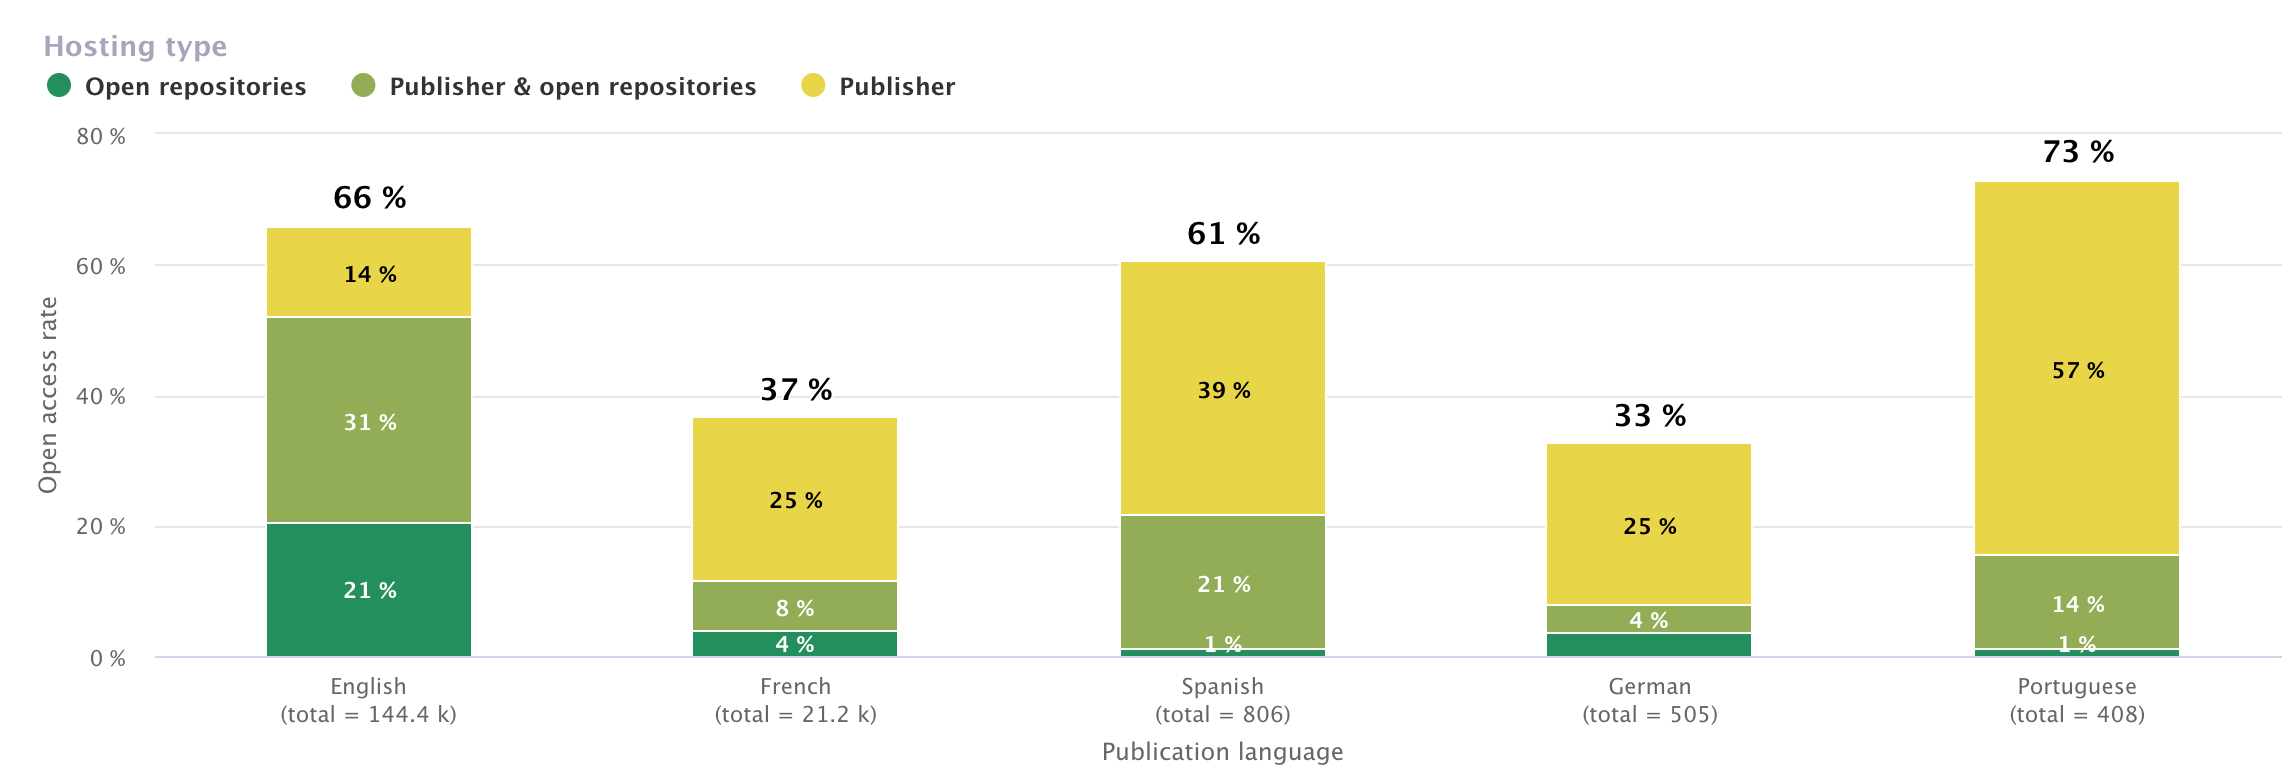
\includegraphics[width=6.25in,height=\textheight]{https://raw.githubusercontent.com/dataesr/bso-publications/main/doc/results_publications_6.png}
\caption{Open access rate by language of publications in France
(publications from 2020)}
\end{figure}

\hypertarget{open-access-dynamics-in-the-different-scientific-fields}{%
\subsubsection{3.1.2 Open access dynamics in the different scientific
fields}\label{open-access-dynamics-in-the-different-scientific-fields}}

The level of openness of publications varies significantly from one
discipline to another, depending on the involvment of scientific
communities and the diversity of their practices. These variations can
also be observed in the trajectory of the level of openness over time.
Some disciplines, such as astronomy and mathematics, have a
long-standing tradition of opening up publications, while others
(chemistry, fundamental biology) have experienced more recent
acceleration. All of them, nevertheless, are part of a dynamic of
openness. There may be artefacts linked to data sources (in SSH and
computer science, some of the publications are not identifiable by our
methodology).

For each year of observation since 2018, the monitor estimates the open
access rate of scientific publications in France published during the
previous year. The figure 13 presents, for each disciplinary field, the
evolution of the open access rate observed each year for the previous
year's publications. This visualization makes it possible to observe and
compare the opening dynamics of the different disciplines: each point on
a line represents the rate observed during an observation year. Thus,
the greater the distance between two consecutive points, the more the
open access rate has evolved between two years of observation. We
observe, for example, that during the last years of observation, it is
the chemistry that marked the largest increase in the rate of open
access publications compared to 2018, going from 28\% to 64\% open.

\begin{figure}
\centering
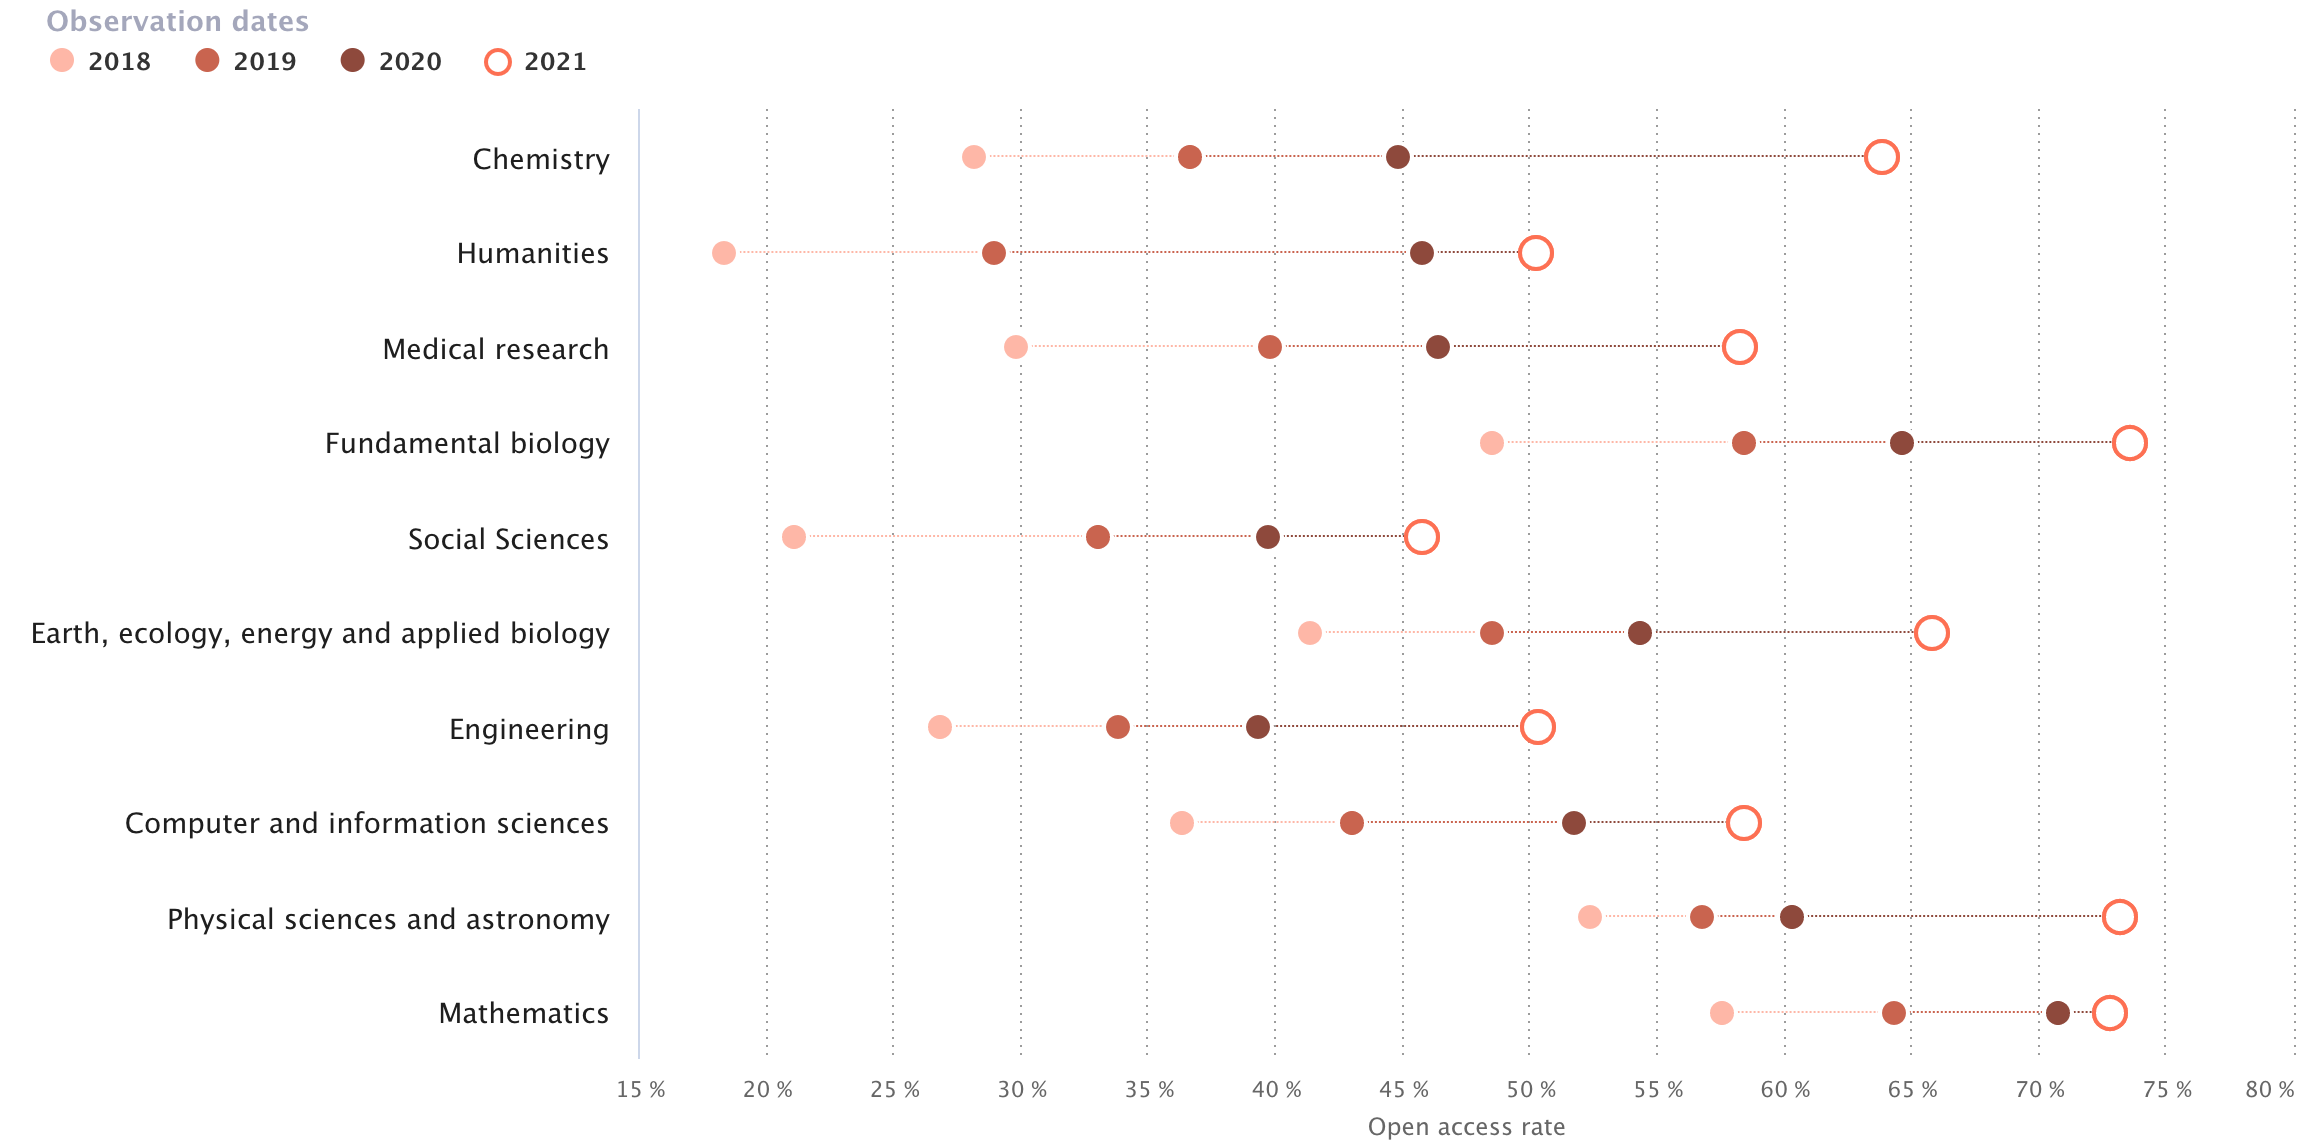
\includegraphics[width=6.25in,height=\textheight]{https://raw.githubusercontent.com/dataesr/bso-publications/main/doc/results_publications_fields_1.png}
\caption{Dynamics of the evolution of the rate of open access
publications in France for each discipline}
\end{figure}

Not all disciplines adopt the same vectors for publishing in open
access. For some, the practice of depositing in an open archive is
historically rooted and legitimate. Mathematicians, physicists and
computer scientists have long practiced open archives upstream of
journal submission. The humanities and social sciences more readily
entrust their openness to publishers. Between the two, there are many
situations, depending on the organization and history of the
disciplines. The most striking fact in the field of biology-health is
the existence of an international policy, initially at the initiative of
organizations funding research projects, which leads to a systematic
deposit, with or without embargo, in PubMed Central (PMC) in the United
States, or Europe PMC in Europe, which means that these disciplines open
up both on the publishers' platforms but also in a globally used open
archive. From the point of view of the National Plan for Open Science,
the cohabitation of the two models (openness via publishers and via open
archives) presents neither contradiction nor disadvantage. On the other
hand, it allows a good resilience of the system.

For each discipline, the figure 14 represents, for publications in
France released in 2020 and at the most recent observation date (2021),
what is the respective share of the different routes to open access:
publication in open access by the publisher, deposit in one or more open
archives, or both routes simultaneously. Note that from one update to
the next, each individual publication may change status, for example
from ``open via publisher'' to ``open via publisher and open archive''
if the publication has been deposited in an open archive in the
meantime. In particular, we note that for publications published in 2020
in medical research, 9\% of publications are open via the open archive
route, 31\% are open via the publisher \& open archive route and 17\%
are open via the publisher route.

\begin{figure}
\centering
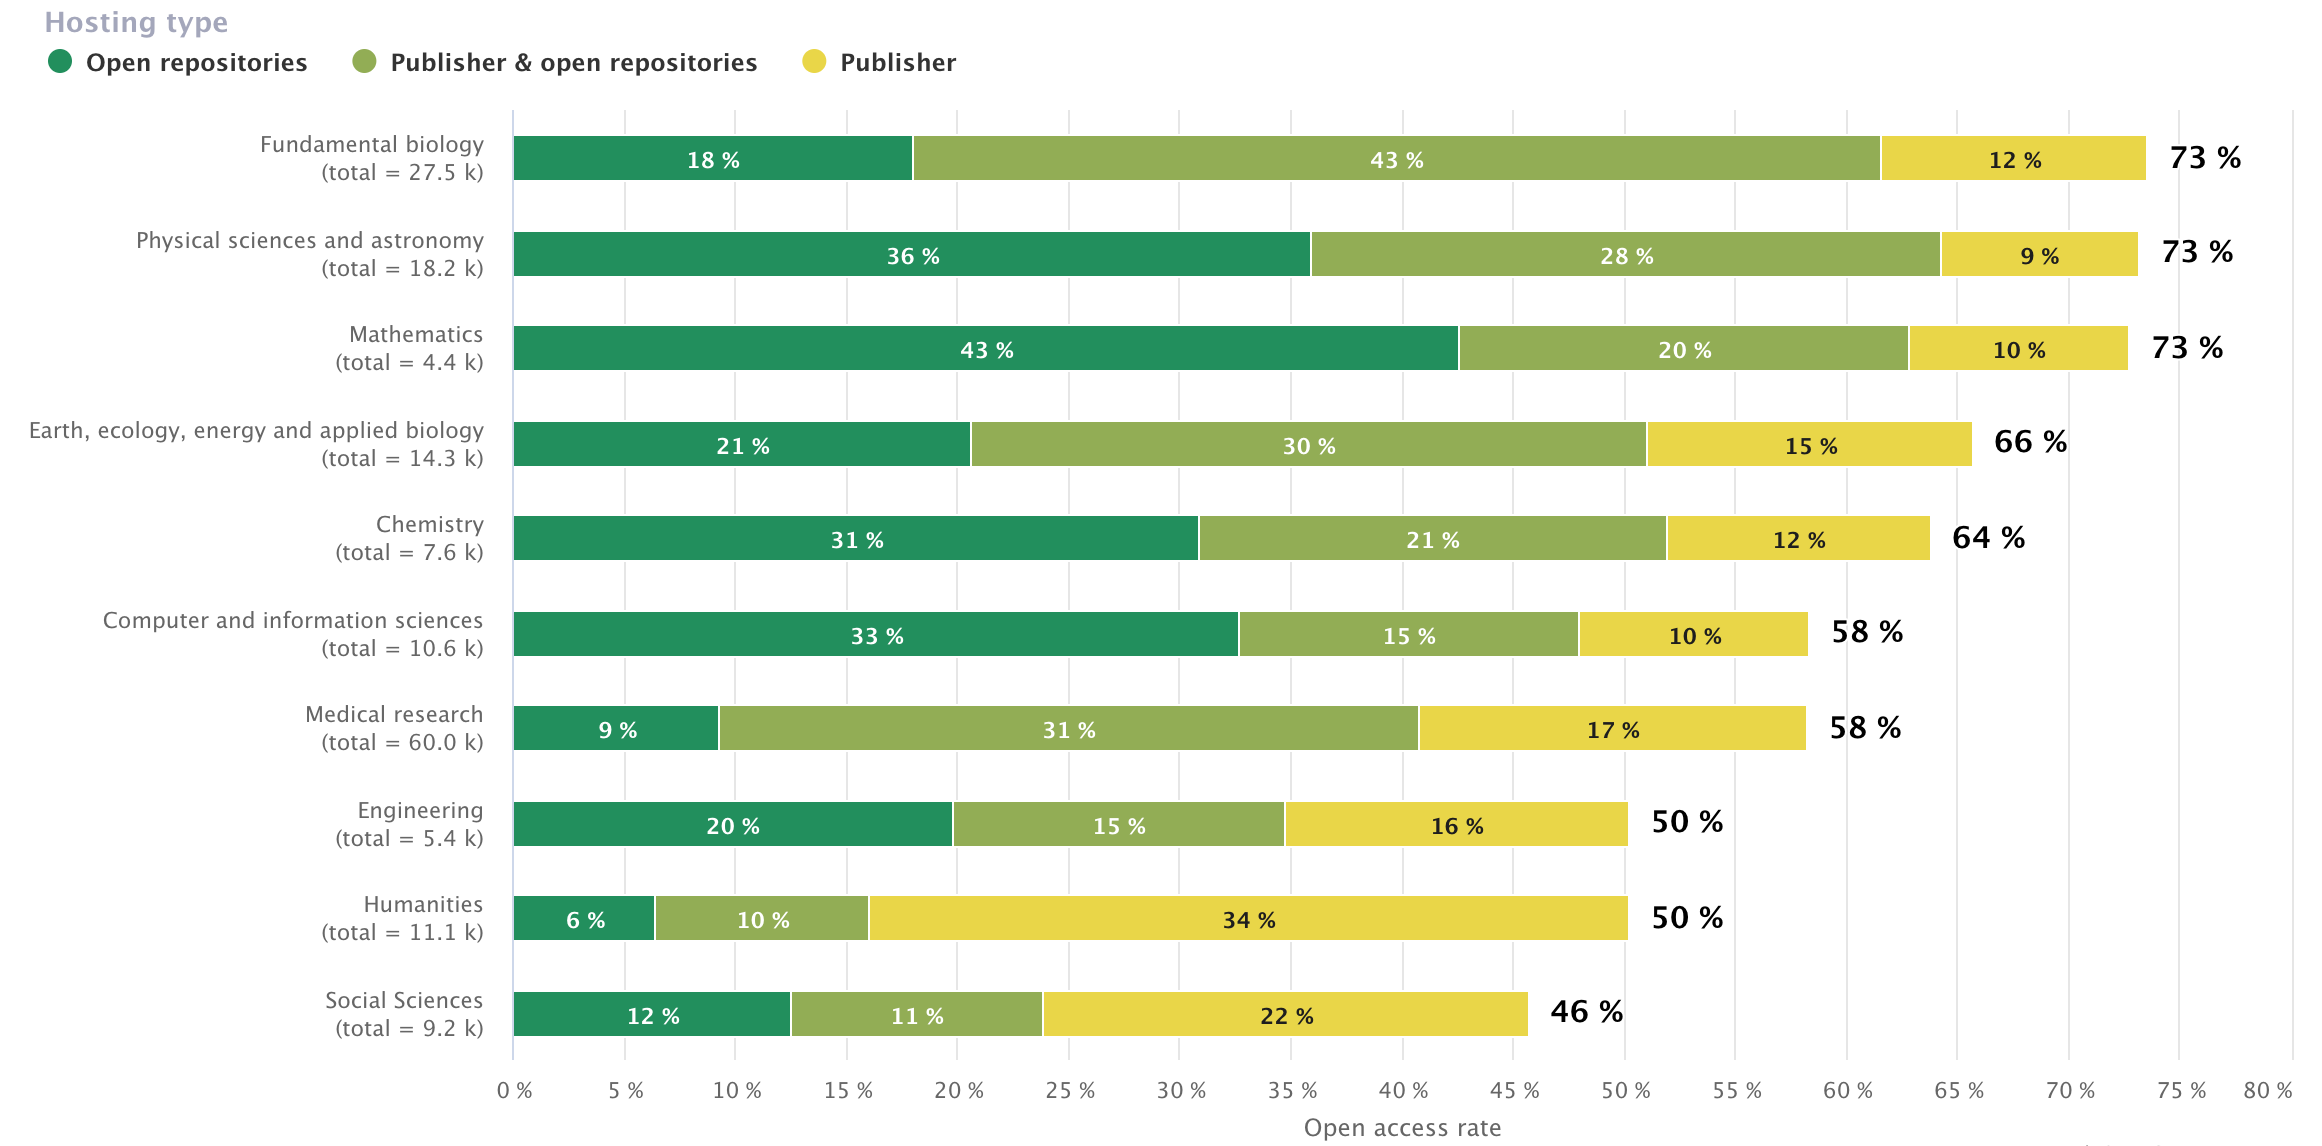
\includegraphics[width=6.25in,height=\textheight]{https://raw.githubusercontent.com/dataesr/bso-publications/main/doc/results_publications_fields_2.png}
\caption{Distribution of publications in France by opening route for
each discipline (publications of 2020)}
\end{figure}

In figure 15, each discipline is represented by a bubble whose size is
proportional to the volume of publications in France released in 2020.
The positioning of the bubble indicates which are the preferred channels
for opening publications in the discipline concerned: the further to the
right the bubble is positioned, the higher the share of publications
opened by the publisher for that discipline; the higher the bubble is
positioned, the higher the share of publications deposited on an open
archive. When the bubble is positioned at the top right of the graph, it
means that publications from this discipline are open simultaneously on
the publisher's publishing platform and on one or more open archives.
Thus, mathematics is very keen on open archives and the humanities are
more willing to entrust their openness to publishers. If the sum of the
share of publications opened by the publisher and the share on open
archive is greater than 100\%, it means that some publications are
deposited in 2 (or more) places at the same time.

\begin{figure}
\centering
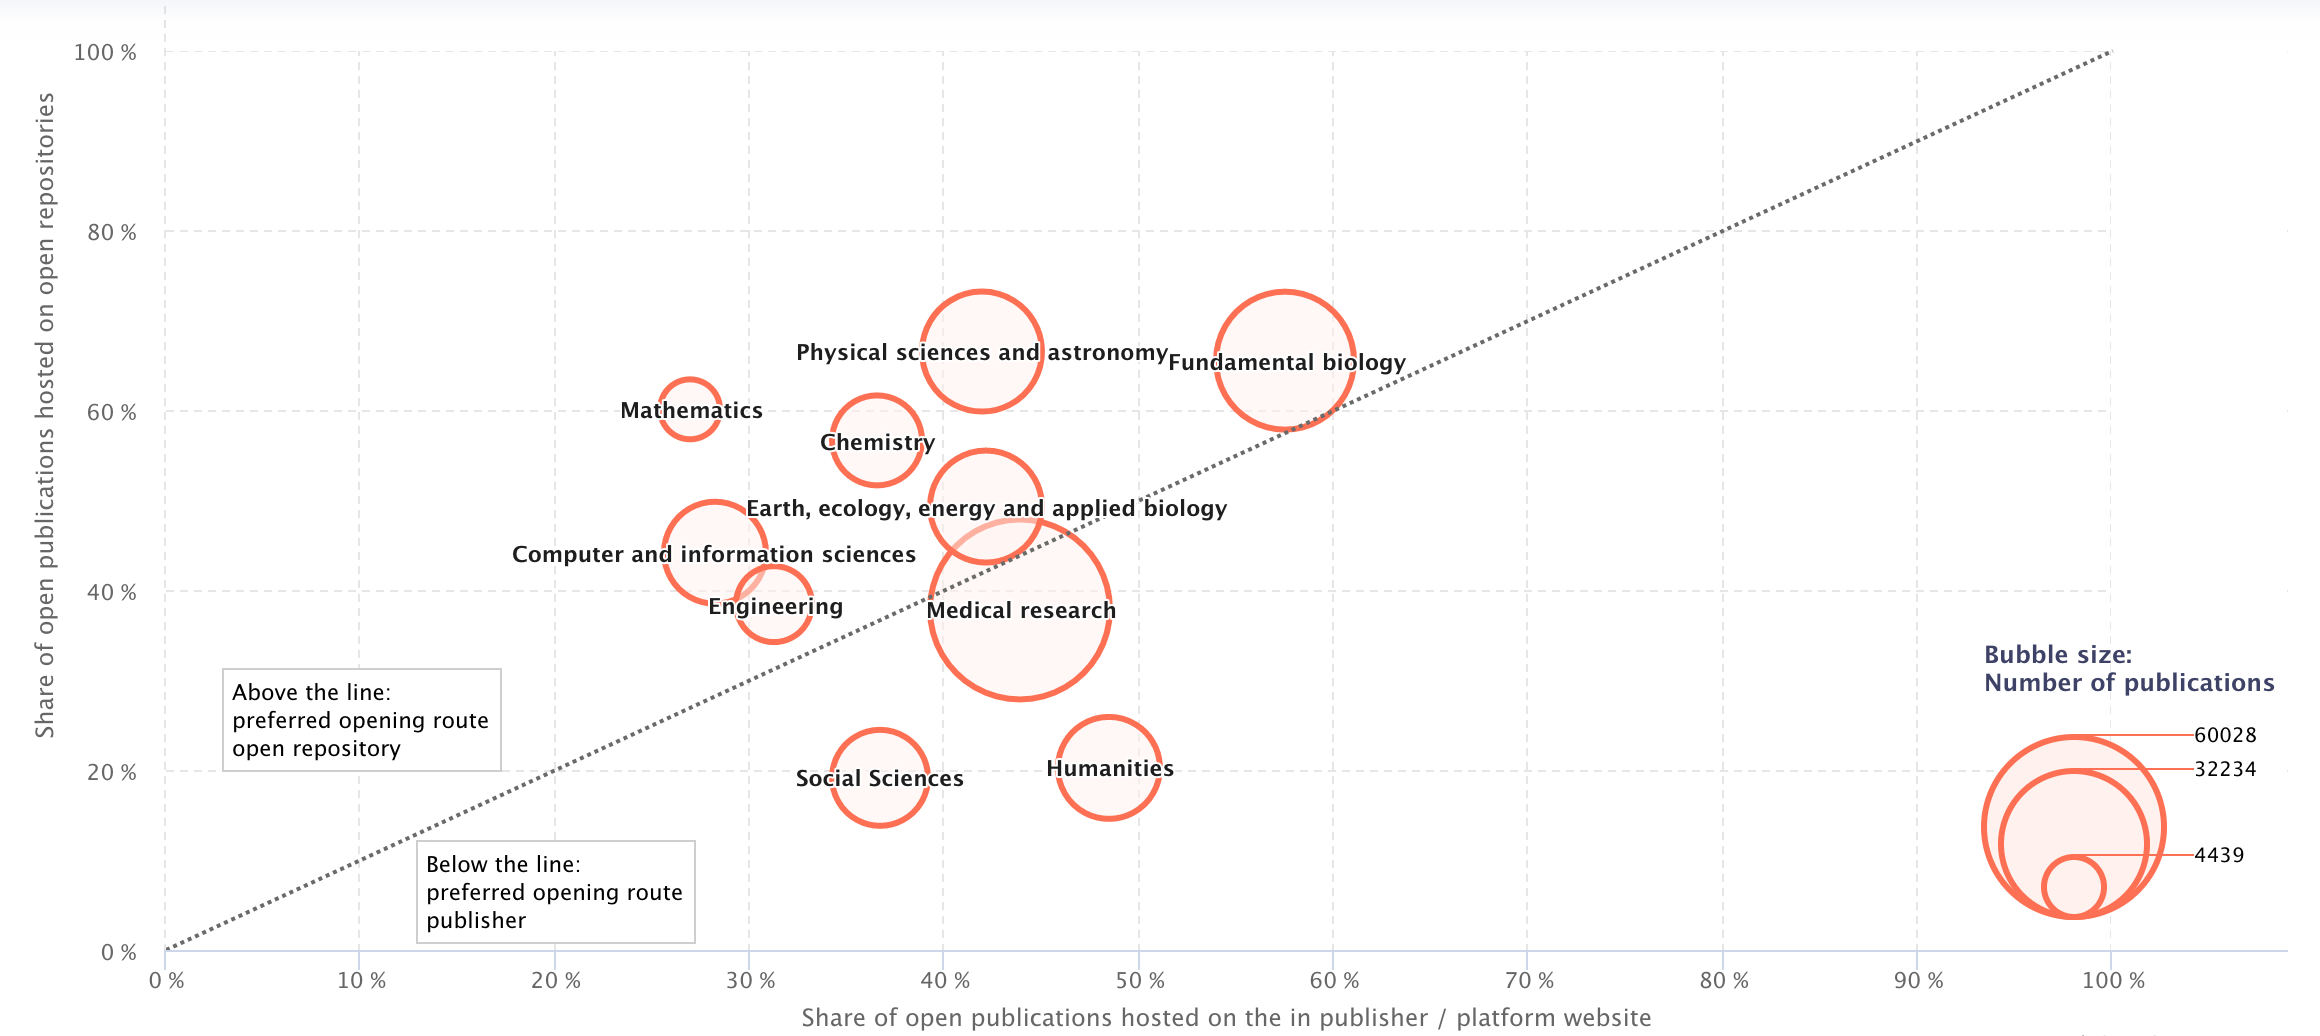
\includegraphics[width=6.25in,height=\textheight]{https://raw.githubusercontent.com/dataesr/bso-publications/main/doc/results_publications_fields_3.png}
\caption{Positioning of disciplines according to the preferred route for
opening their publications in France (publications of 2020)}
\end{figure}

\hypertarget{open-access-dynamics-and-publishers-policies}{%
\subsubsection{3.1.3 Open access dynamics and publishers
policies}\label{open-access-dynamics-and-publishers-policies}}

The global publishing landscape is extremely diverse. There are about
12,000 scientific publishers around the world, each with a different
history. They may be commercial or not-for-profit, national or
multinational publishing companies, scholarly societies, university
presses with public status, etc. Some actors have chosen to publish in
open access from the start, while others have more or less strongly and
recently engaged in a transition towards open access, with various
models. There is a shared tendency to publish more and more in open
access. We are not measuring here the open access rate of French
publishers, but of the publishers in which French researchers publish.
Nor do we measure the gradual reduction in the duration of moving
barriers.

For each year of observation since 2018, the graph represents the share
of scientific publications in France published during the previous year
that are made available in open access by their publisher. Some of these
publications may be simultaneously available in an open archive. On the
other hand, publications that are only available via an open archive are
not taken into account. Thus, in 2021, 44\% of scientific publications
in France released in 2020 were made available in open access by their
publisher (figure 16).

\begin{figure}
\centering
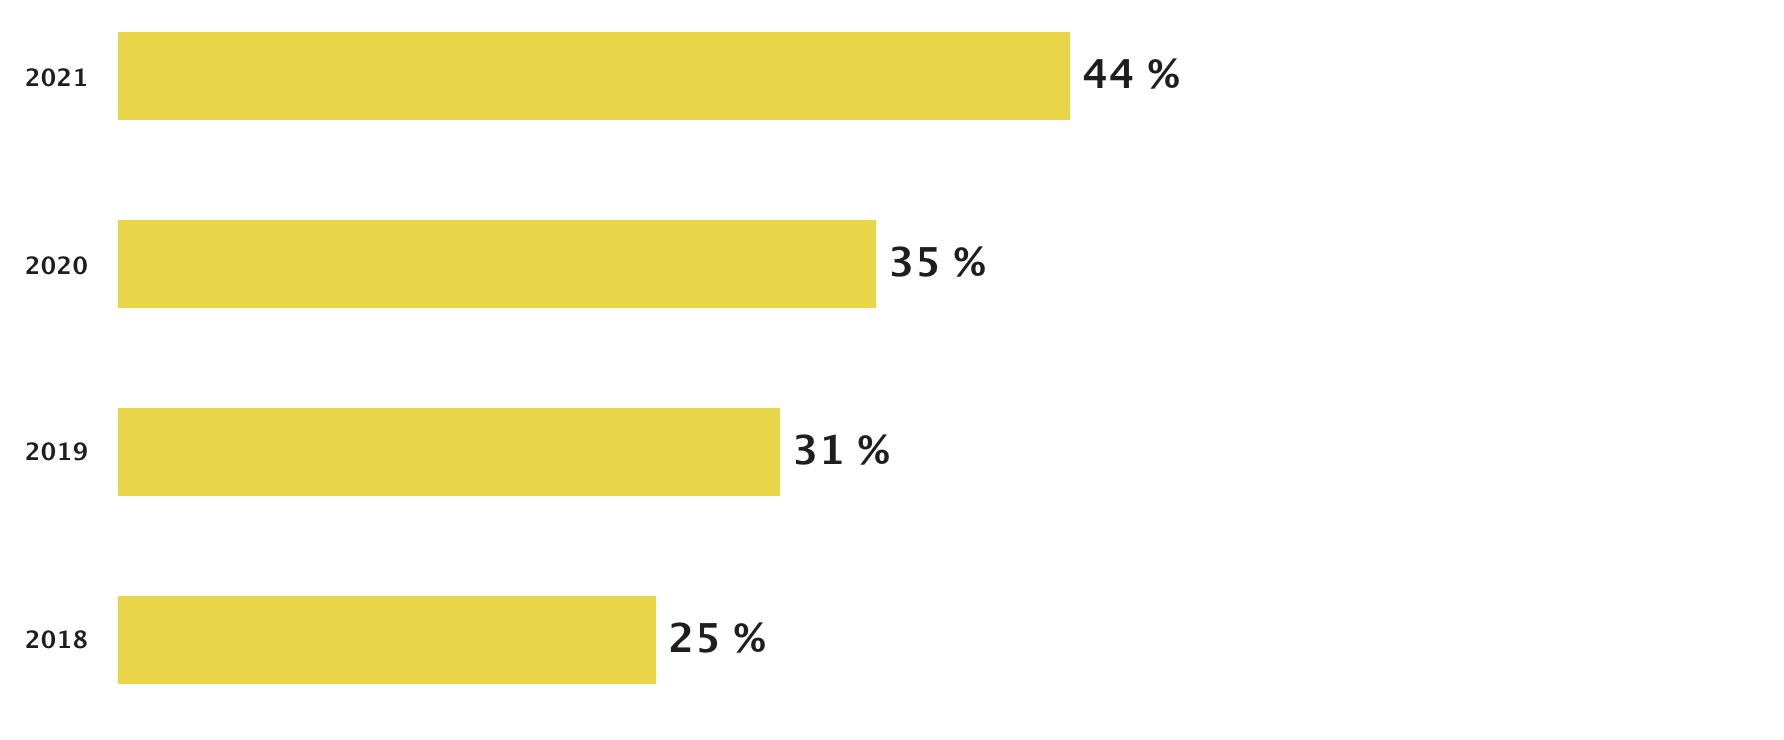
\includegraphics[width=6.25in,height=\textheight]{https://raw.githubusercontent.com/dataesr/bso-publications/main/doc/results_publications_publishers_1.png}
\caption{Share of scientific publications in France made available in
open access by their publisher, by year of observation, for publications
published during the previous year}
\end{figure}

In figure 17, for each observation year and by publication date, the
share of scientific publications in France that are made available in
open access by their publisher is displayed. Each line represents the
rates observed at an observation date, and the rates are expressed as a
function of the volume of publications published in the year observed.
It can be seen that, for publications released in a given year, the rate
of open access by the publisher varies from one observation date to
another. This is due, for example, to the process of releasing the most
recent publications through the expiry of moving barriers. Thus, between
2018 and 2021, the share of publications released in 2017 that are made
available in open access by their publisher has increased from 25\% to
33\%.

\begin{figure}
\centering
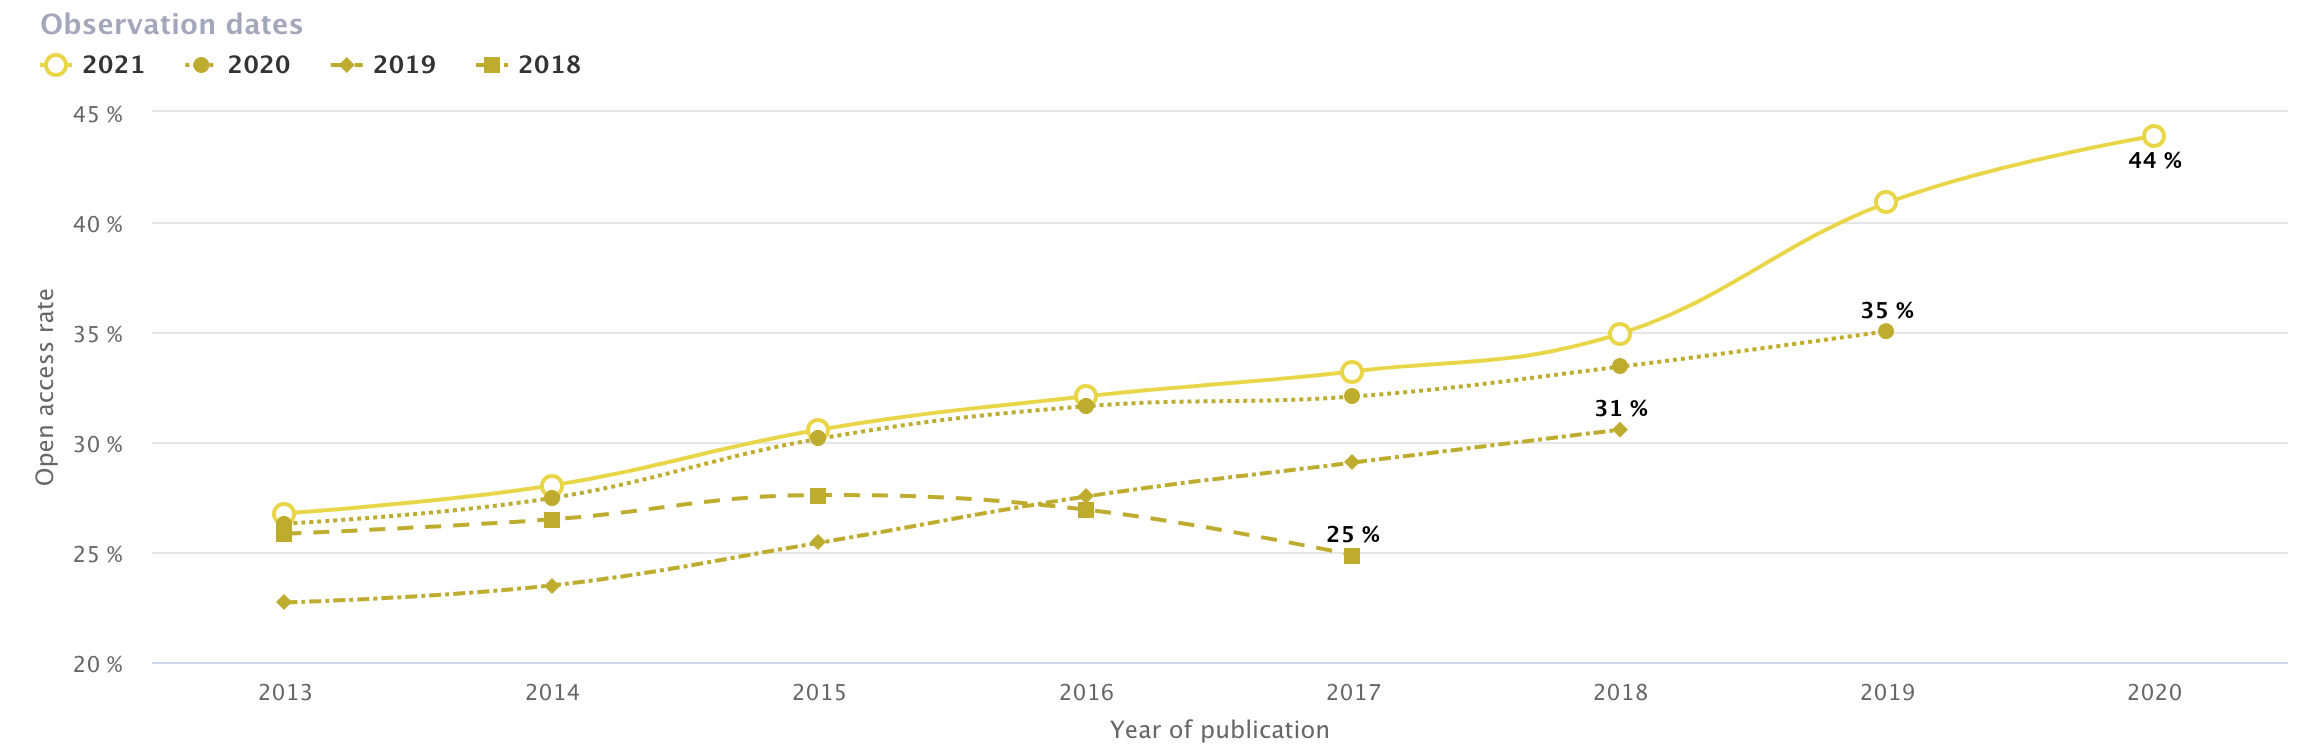
\includegraphics[width=6.25in,height=\textheight]{https://raw.githubusercontent.com/dataesr/bso-publications/main/doc/results_publications_publishers_2.png}
\caption{Evolution of the share of publications in France made available
in open access by publisher by year of observation}
\end{figure}

The dissemination of open access articles by academic journal publishers
is based on various business models. Some publishers have replaced
traditional subscription revenues with the payment of publication fees
(APC) charged on a per-article basis to researchers, their institutions
or their funders. This change of model is often done at the level of an
entire journal (full APC model), but other publishers maintain the
subscription while offering authors the choice to open their article in
return for the payment of a publication fee (a model known as hybrid),
thus establishing a particularly unreadable double payment. Some
publishers do not charge publication fees but mobilize, in the context
of a non-commercial activity, funding from states, public actors,
universities or other non-profit organisations, in order to finance the
editorial and publication activity upstream: this is the so-called
diamond OA model (Bosman et al. (2021)). Finally, other models exist,
such as the one where the publisher collects subscriptions for the most
recent publications while releasing them in open access after a set
period of time (moving barrier).

The figure 18 shows the distribution of scientific articles published in
2020 and distributed in open access by their publisher, according to the
business model of the journal in which they are published. It
distinguishes between four types of economic models: articles published
in full open access journals that do not charge publication fees
(``diamond''), articles published in full open access journals that do
charge publication fees (``Gold full APC''), and articles published in
hybrid journals (where only some part of the content is in open access
and the other part is available through individually paid publication
fees), and all other cases. The ``Diamond'' part is probably
underestimated. In particular, we observe that for scientific
publications in France released in 2020, diamond represents 9\% of the
articles disseminated in open access by their publisher.

\begin{figure}
\centering
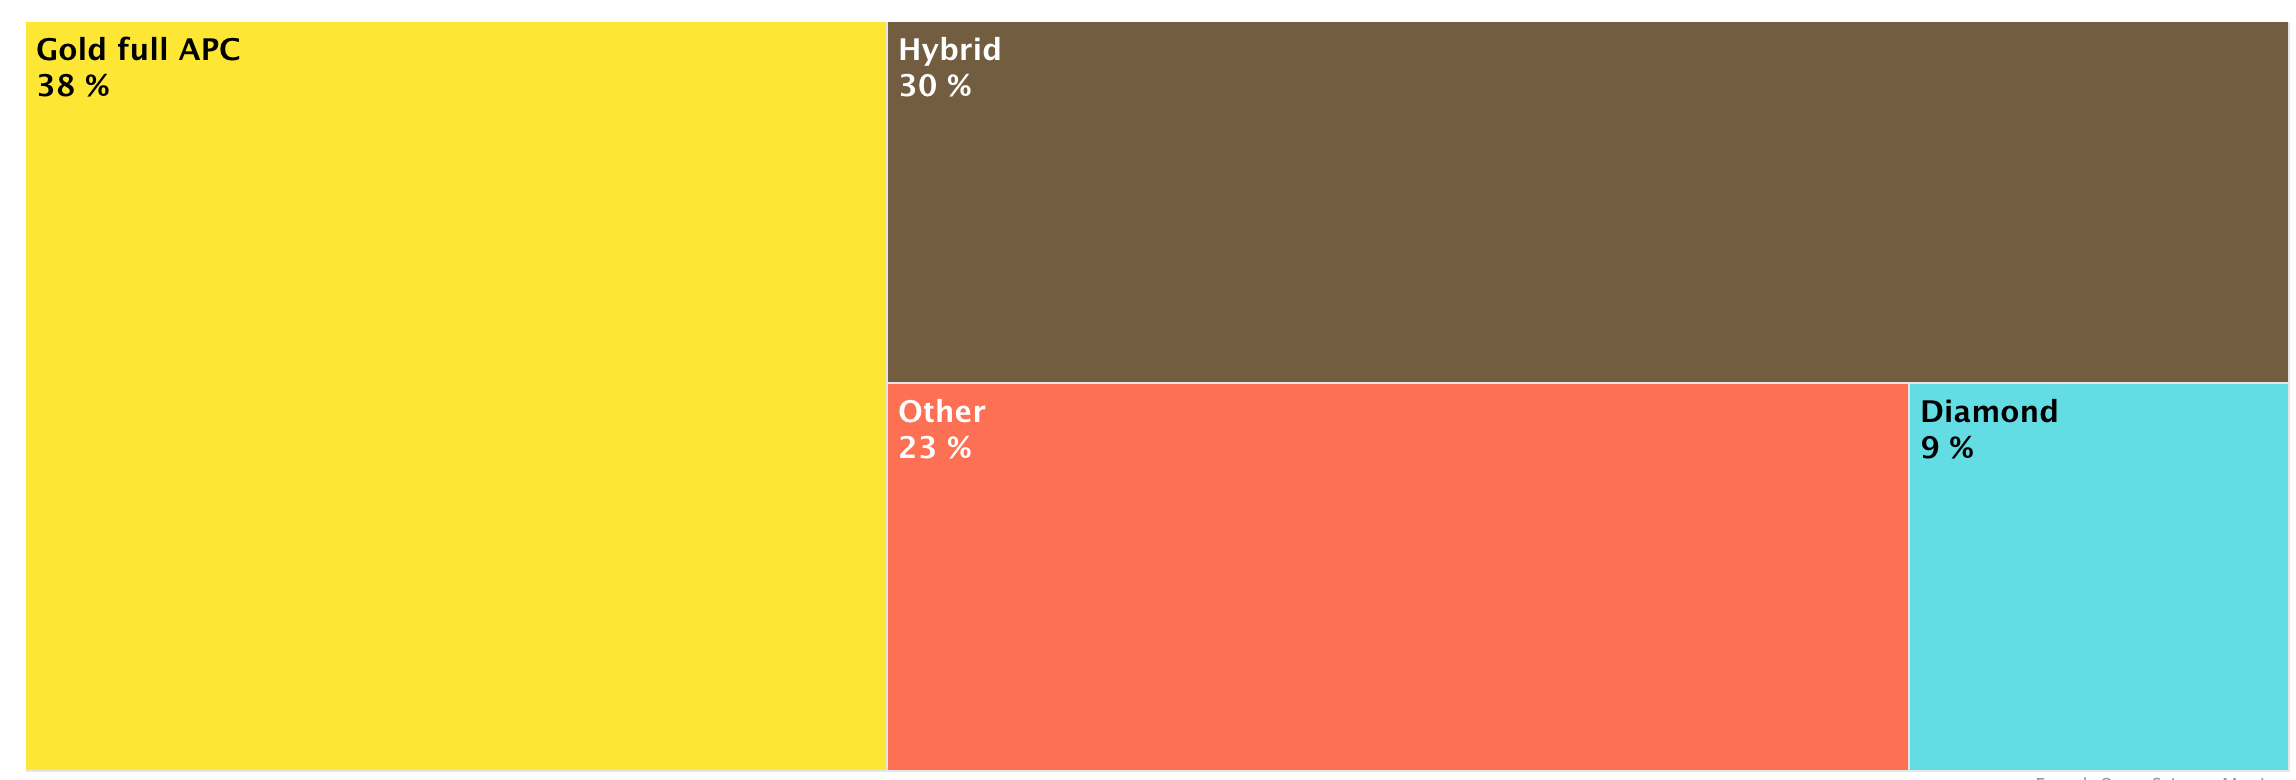
\includegraphics[width=6.25in,height=\textheight]{https://raw.githubusercontent.com/dataesr/bso-publications/main/doc/results_publications_publishers_3.png}
\caption{Distribution of business models for articles published in 2020
and distributed in open access by their publisher}
\end{figure}

In 2016, the French law for a Digital Republic made it possible for
researchers who have published a scientific article with a publisher to
deposit the accepted version of the article for publication in an open
repository, subject to a time limit (embargo) that can be set by the
publisher but cannot exceed 6 months for science, technology and
medicine and 12 months for the humanities and social sciences. Deposit
in an open archive is therefore a way to counterbalance the restrictive
open access policy of some publishers and it plays a decisive role in
providing access for all to French research results. Conversely, when
the publisher publishes natively in open access, deposit in an open
archive may appear less necessary to authors. However, it remains useful
and desirable. Indeed, a deposit on the national open archive HAL
guarantees the perennial conservation of the content and the control of
the results of French scientific research, regardless of the hazards
that affect publishers or their distribution platforms.

\begin{figure}
\centering
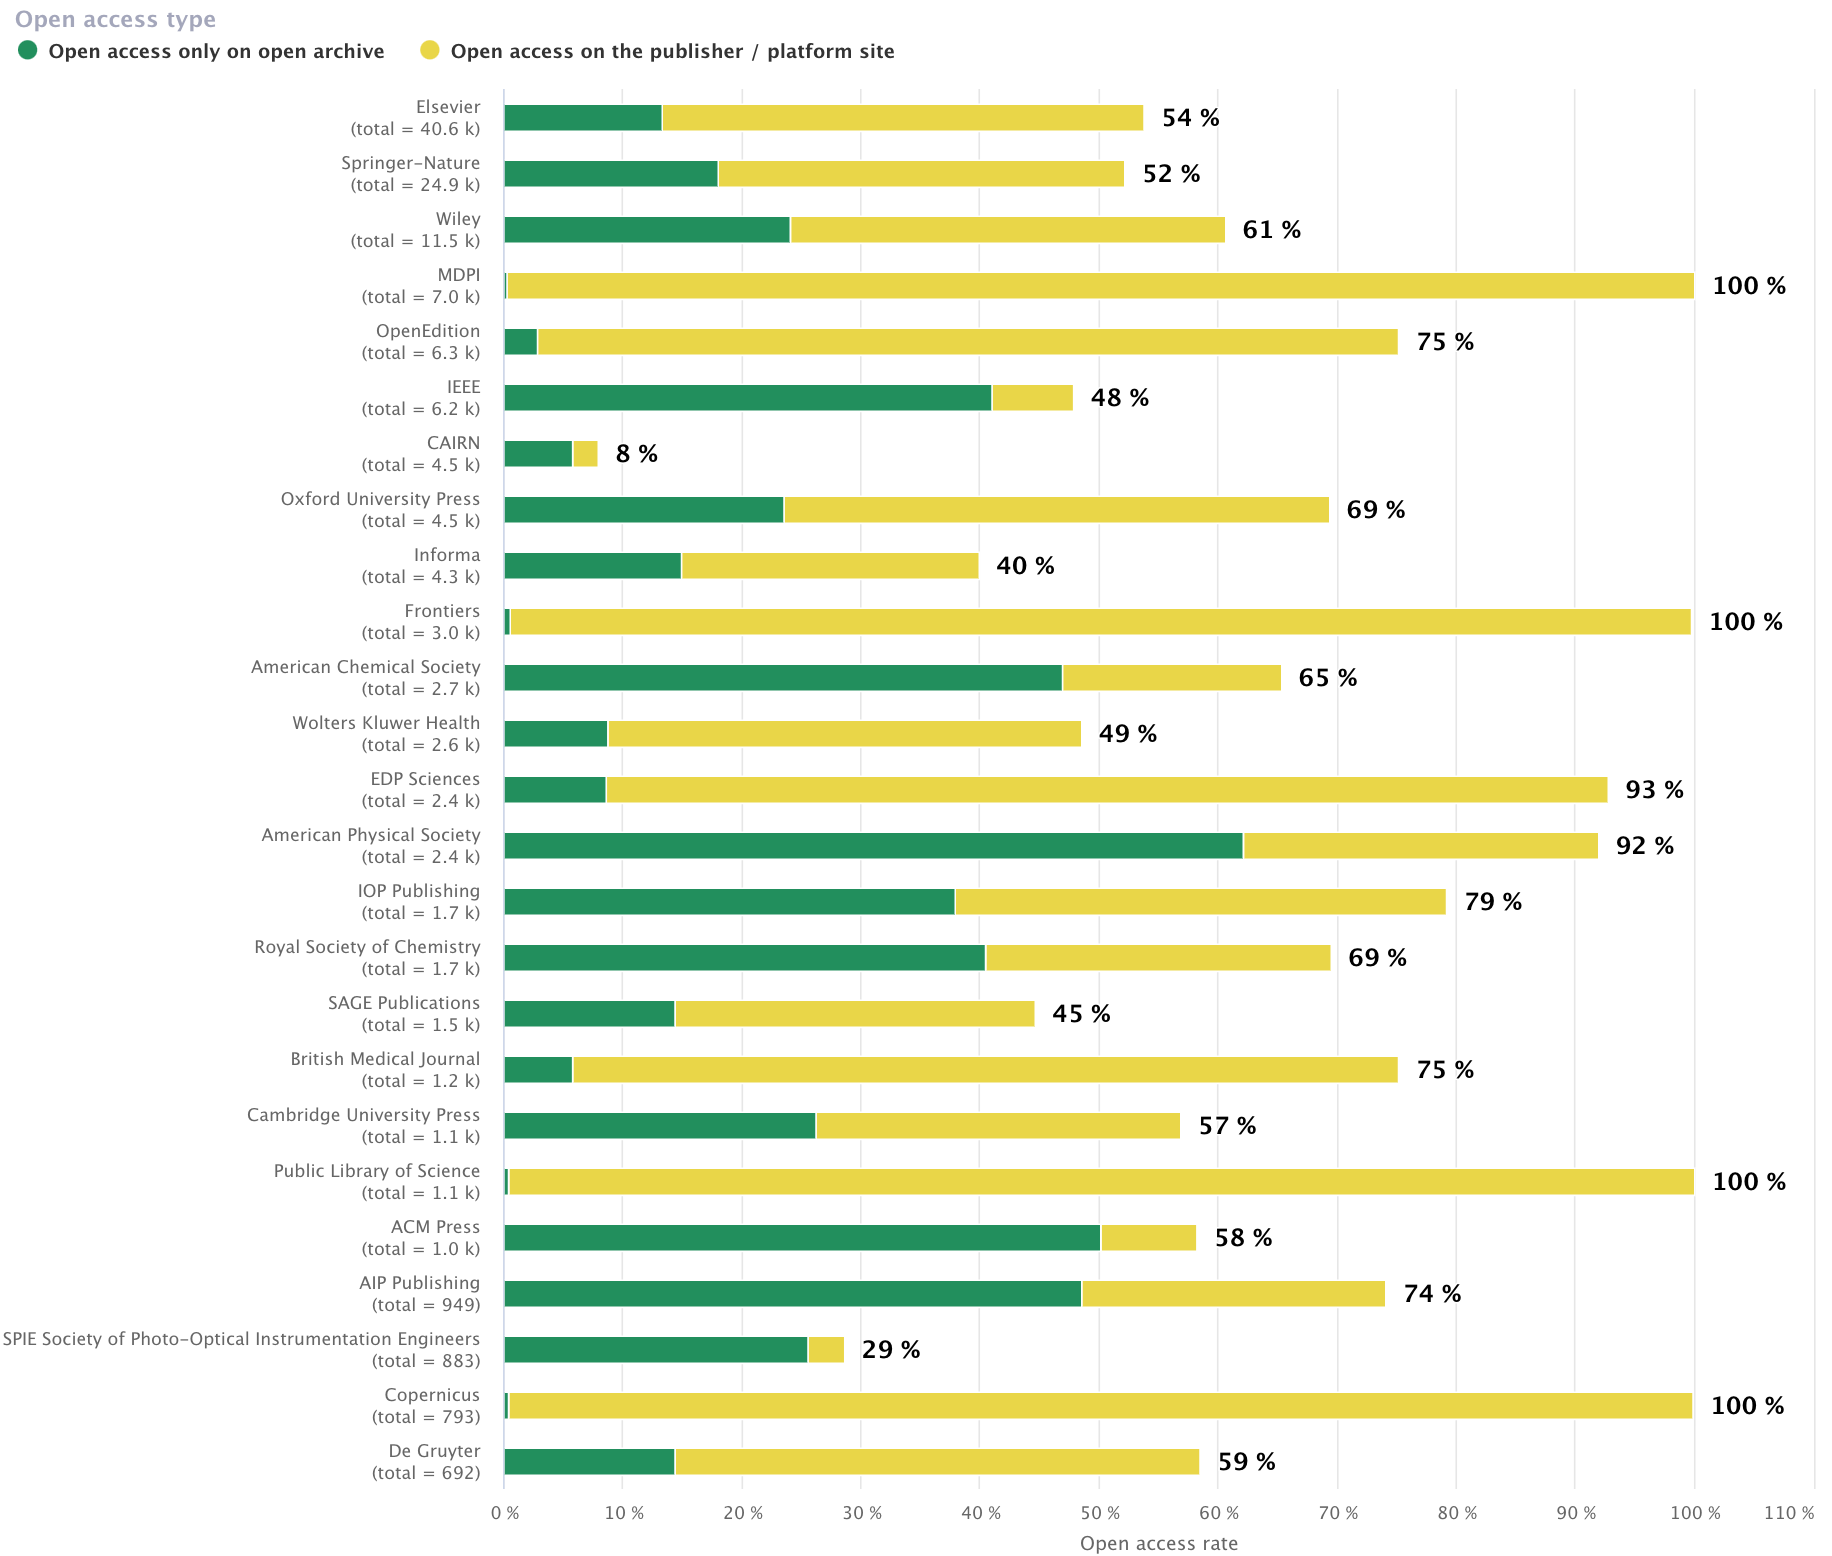
\includegraphics[width=6.25in,height=\textheight]{https://raw.githubusercontent.com/dataesr/bso-publications/main/doc/results_publications_publishers_4.png}
\caption{Opening routes for scientific publications in France released
in 2020 by the most important publishers or publishing platforms in
terms of volume (top 25)}
\end{figure}

\begin{figure}
\centering
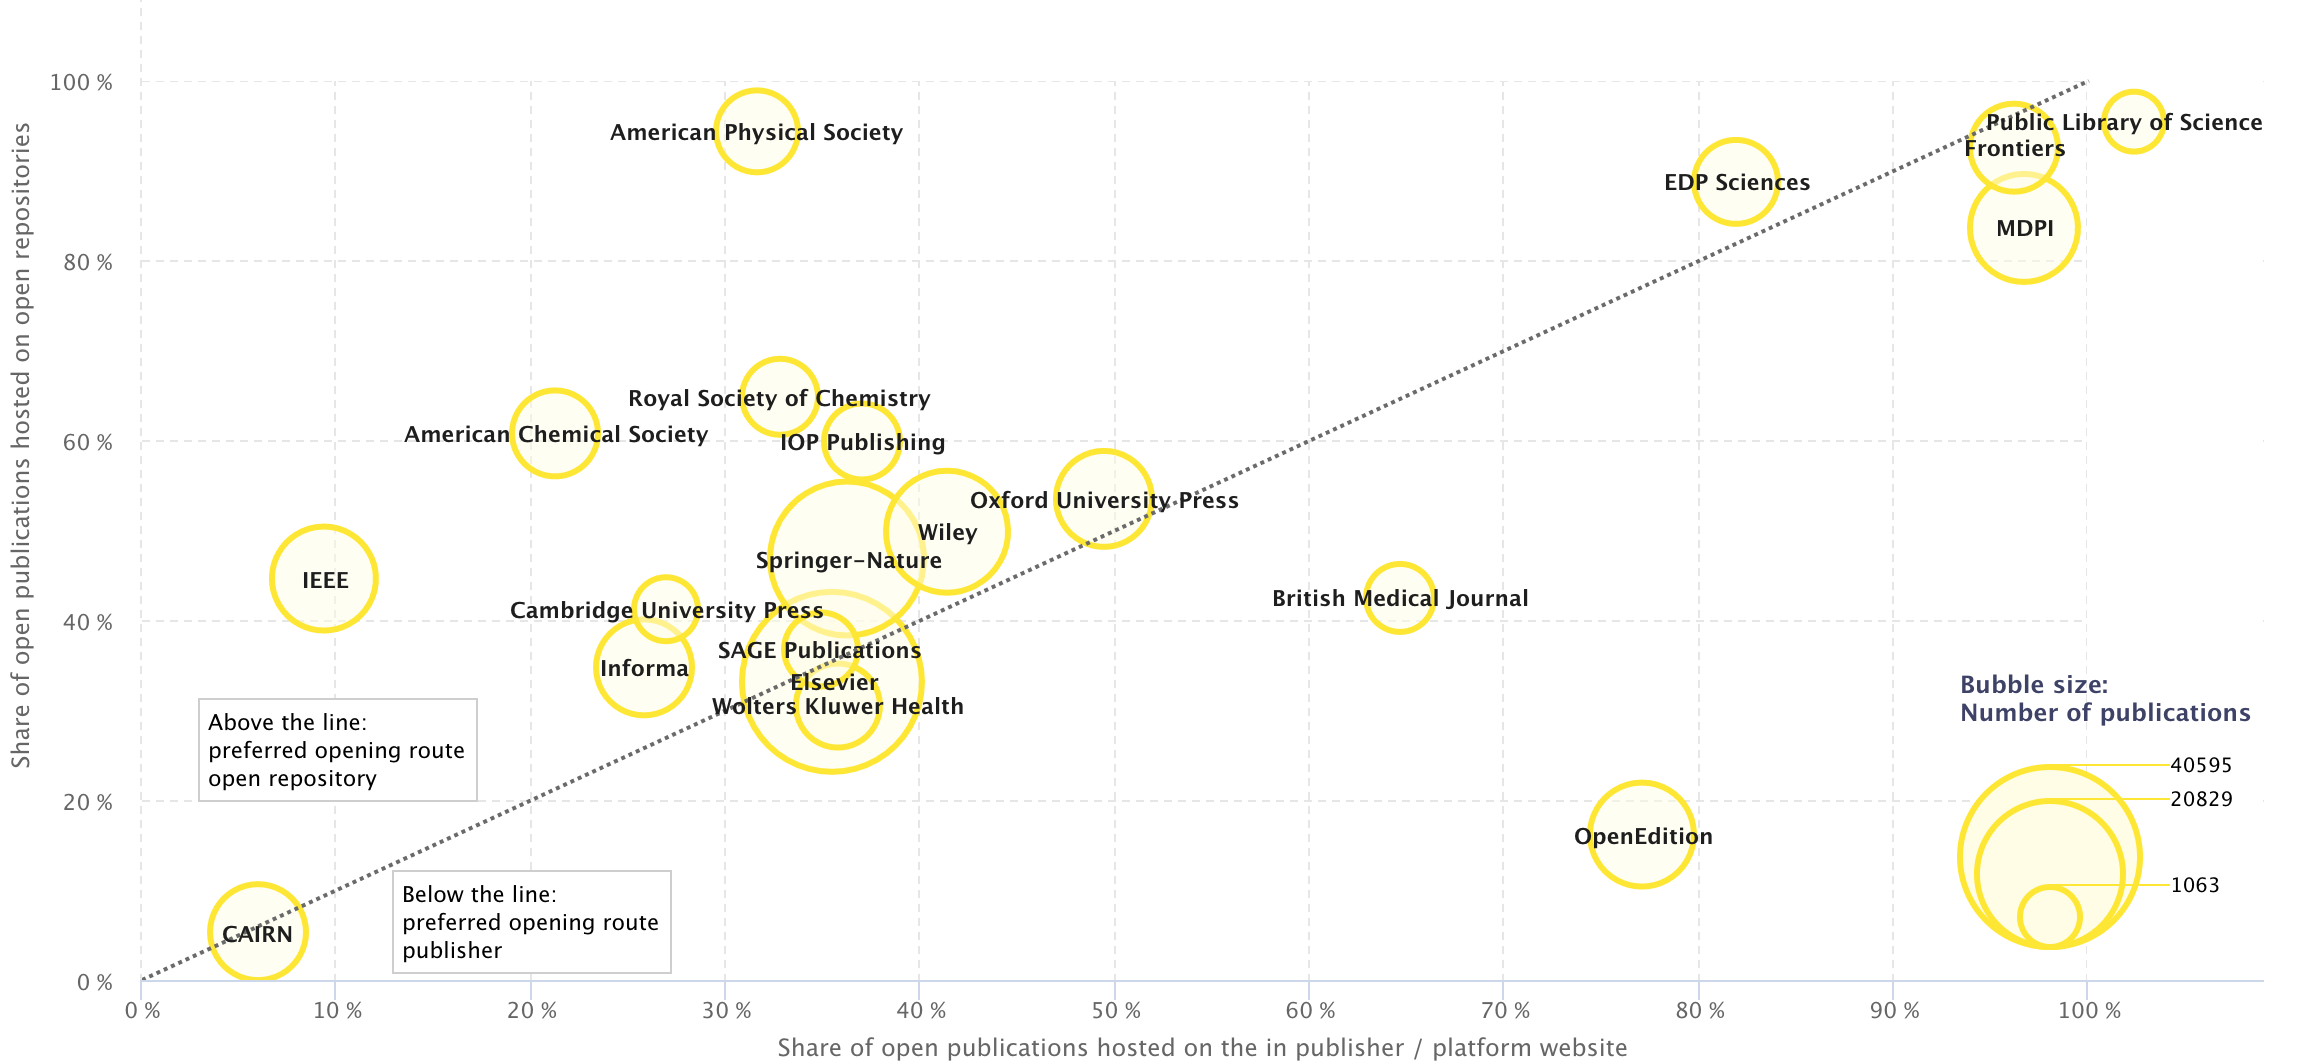
\includegraphics[width=6.25in,height=\textheight]{https://raw.githubusercontent.com/dataesr/bso-publications/main/doc/results_publications_publishers_5.png}
\caption{Positioning of publishers and publishing platforms according to
the preferred route for opening up the French publications they
distribute}
\end{figure}

Open access to scientific publications implies not only the possibility
to read them without having to overcome price or technical barriers, but
also the possibility to reuse them by citing their author(s). The
precise conditions of reuse are defined by means of licences, in
particular the Creative Commons licences that are most commonly used.
Thus publishers implementing an open science policy should not only
release publications in open access, but also attach a free licence
securing the reuse of the content by readers, whether they are
researchers, teachers, professionals or other social actors. The use of
licences thus facilitates the dissemination of scientific knowledge
above and beyond academic communities.

The figure 21 indicates, for scientific publications in France released
in 2020 and distributed in open access by their publisher, what
proportion is accompanied by an open licence specifying the conditions
of re-use. The `See details' button allows a more detailed view of the
type of licence used, in particular for Creative Commons licences. It is
possible to select a publisher or a publication platform (when several
publishers use the same platform, the platform level has been
preferred). Thus, 65\% of scientific publications in France released in
2020 that are distributed in open access by their publisher are
accompanied by an open licence. Within the open licences, the CC-BY
licence is the most popular with 45\% of the publications.

\begin{figure}
\centering
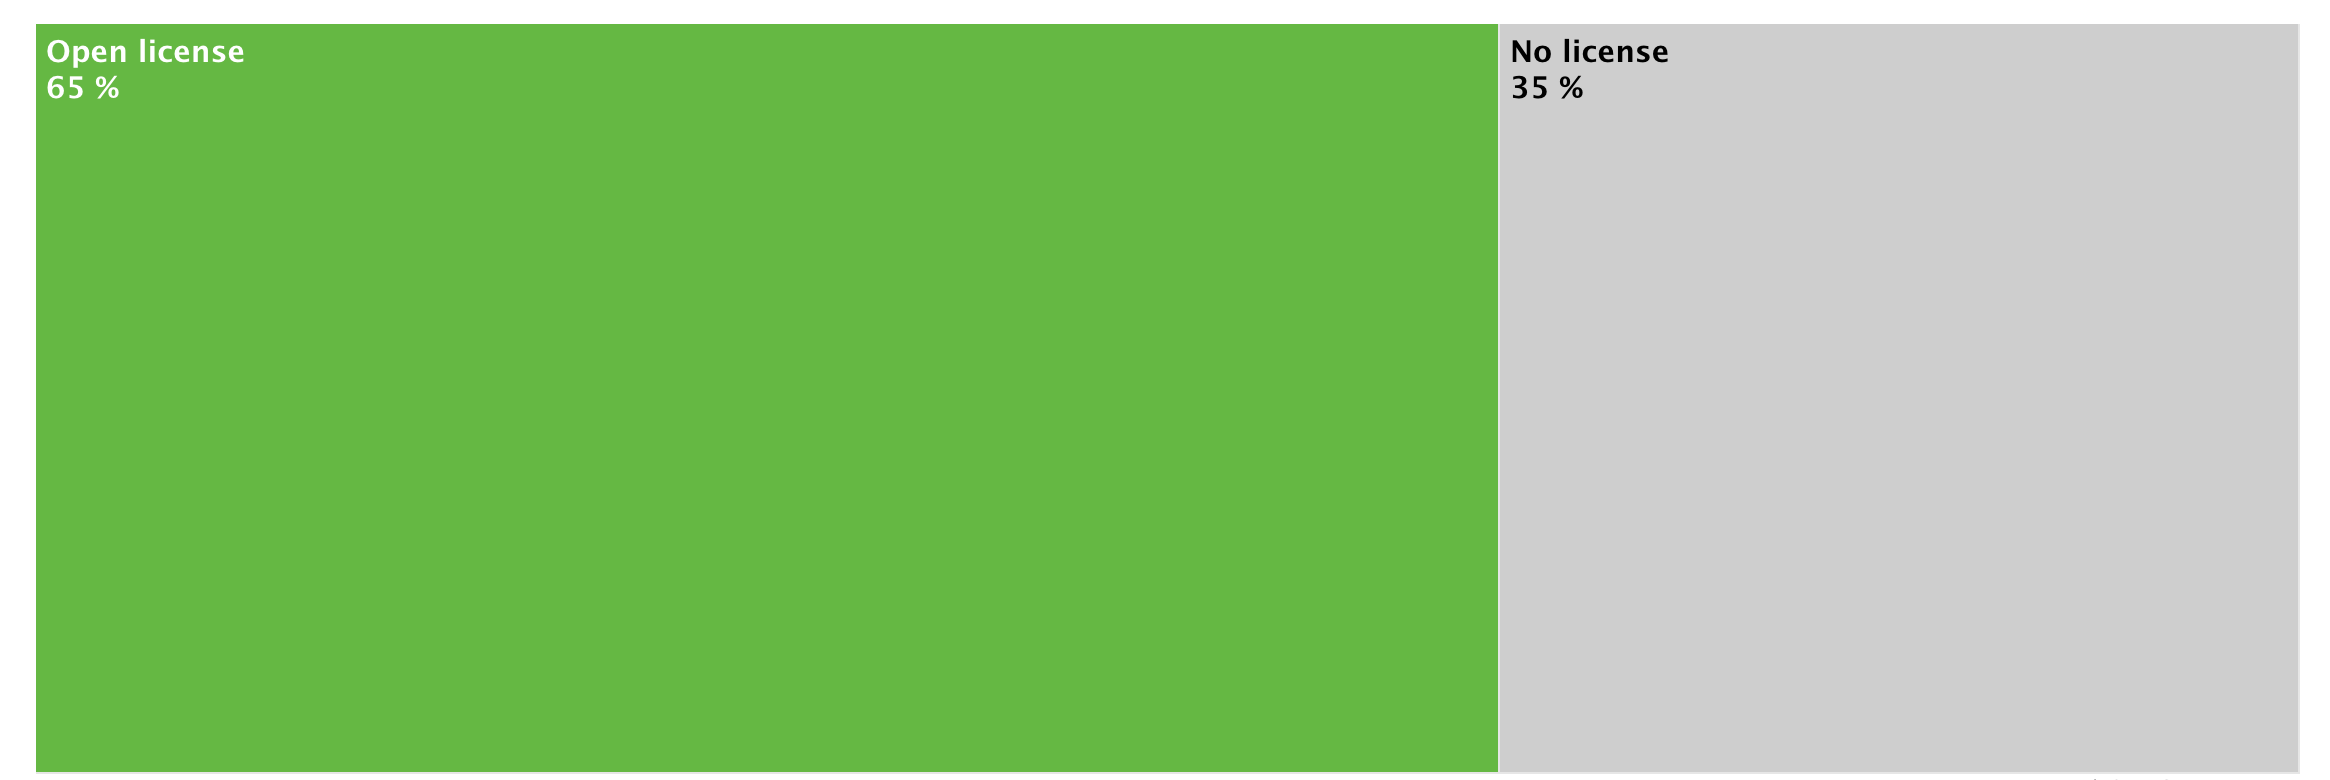
\includegraphics[width=6.25in,height=\textheight]{https://raw.githubusercontent.com/dataesr/bso-publications/main/doc/results_publications_publishers_6.png}
\caption{Distribution of open scientific publications in France by type
of licence used}
\end{figure}

The figure 22 indicates, for each academic publisher or publishing
platform in open access in 2020, the proportion of them that are
accompanied by an open licence. The 25 publishers or platforms
publishing the most French scientific articles in open access are taken
into consideration, in decreasing order. When several publishers use the
same publication platform, the platform level was taken into
consideration. Please note that without a licence, the normal copyright
applies. Thus, Elsevier put an open licence for 28\% of its French open
access publications published in 2020.

\begin{figure}
\centering
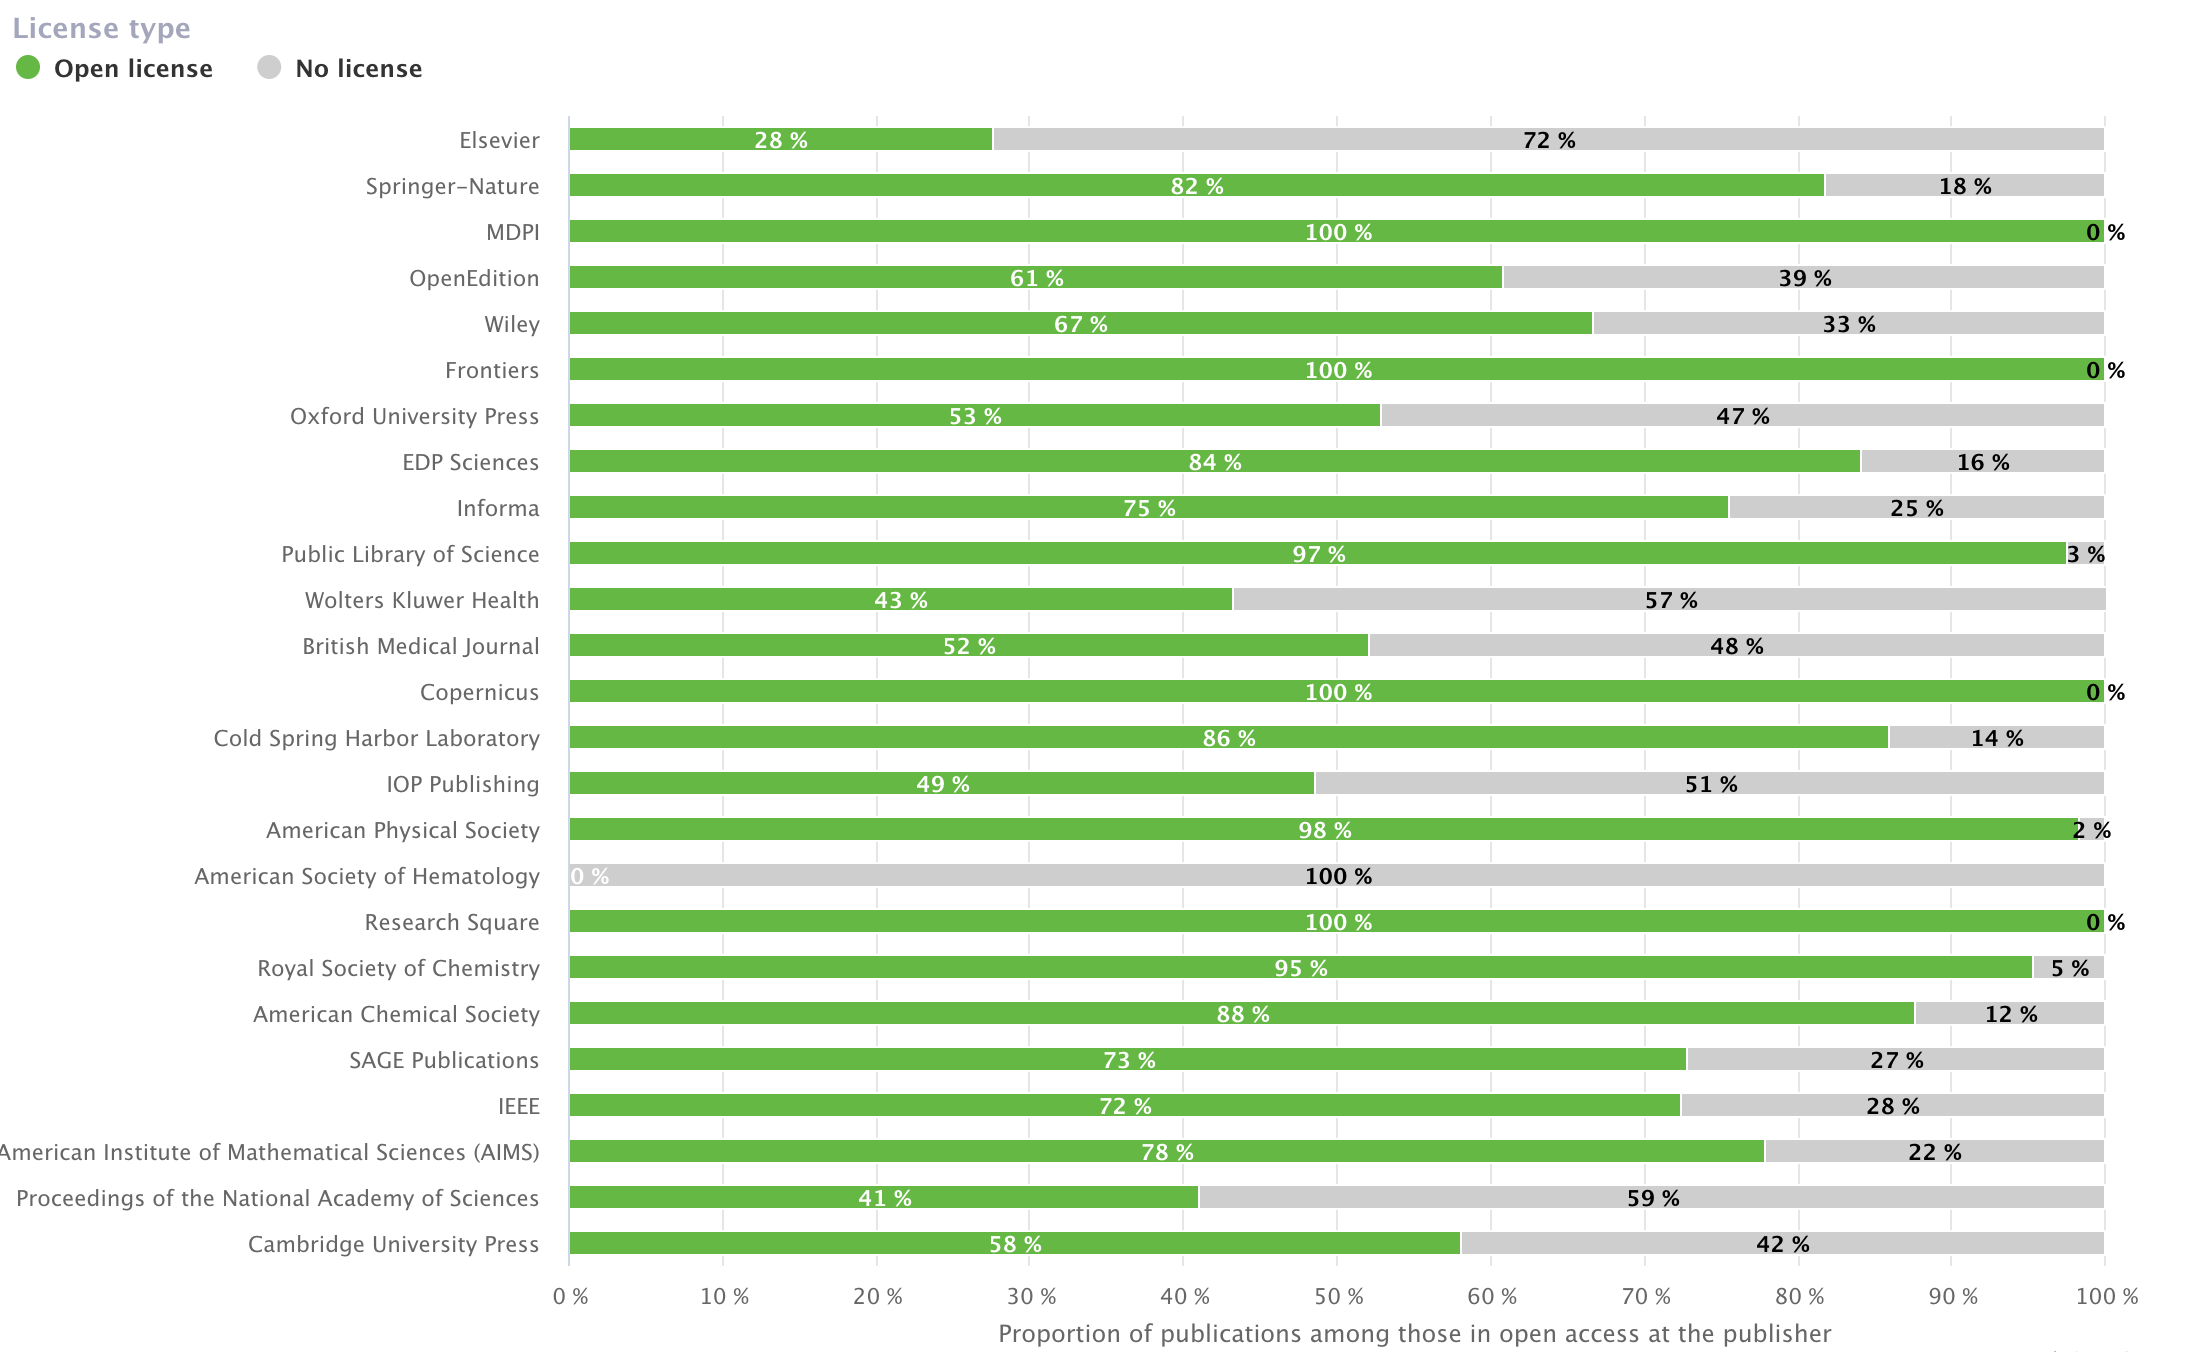
\includegraphics[width=6.25in,height=\textheight]{https://raw.githubusercontent.com/dataesr/bso-publications/main/doc/results_publications_publishers_7.png}
\caption{Rate of use of an open licence by the publishers or publishing
platforms that distribute the most scientific publications in France in
open access (top 25, 2020 publications)}
\end{figure}

One model for financing open access to scientific publications is based
on the payment of publication fees (APC) which publishers charge per
article and which are paid by researchers, their institutions or their
funders. This model is mostly used by commercial publishers, would they
be native OA or have transitioned from subscription models. It is very
expensive and uncertain for public research institutions, especially as
it is accompanied by an inflation in the number of articles published.
It should be weighed against other virtuous economic models - in
particular the ``diamond'' model - which allows greater cost control and
equity in access to publication for researchers.

The figure 23 shows the distribution of scientific publications in
France released in 2020 and in open access by their publisher for a
publication fee, according to the price applied (APC amount). Each point
on a curve represents a volume of publications released for a given APC
rate band. A distinction is made between the curve representing
publications released in journals where all content is open access (Gold
full APC) and the curve representing publications released in hybrid
journals, where only part of the content is in open access while the
rest is subject to subscription. It is possible to view the distribution
for each publisher or publishing platform. When several publishers use
the same publishing platform, the platform level has been privileged.

\begin{figure}
\centering
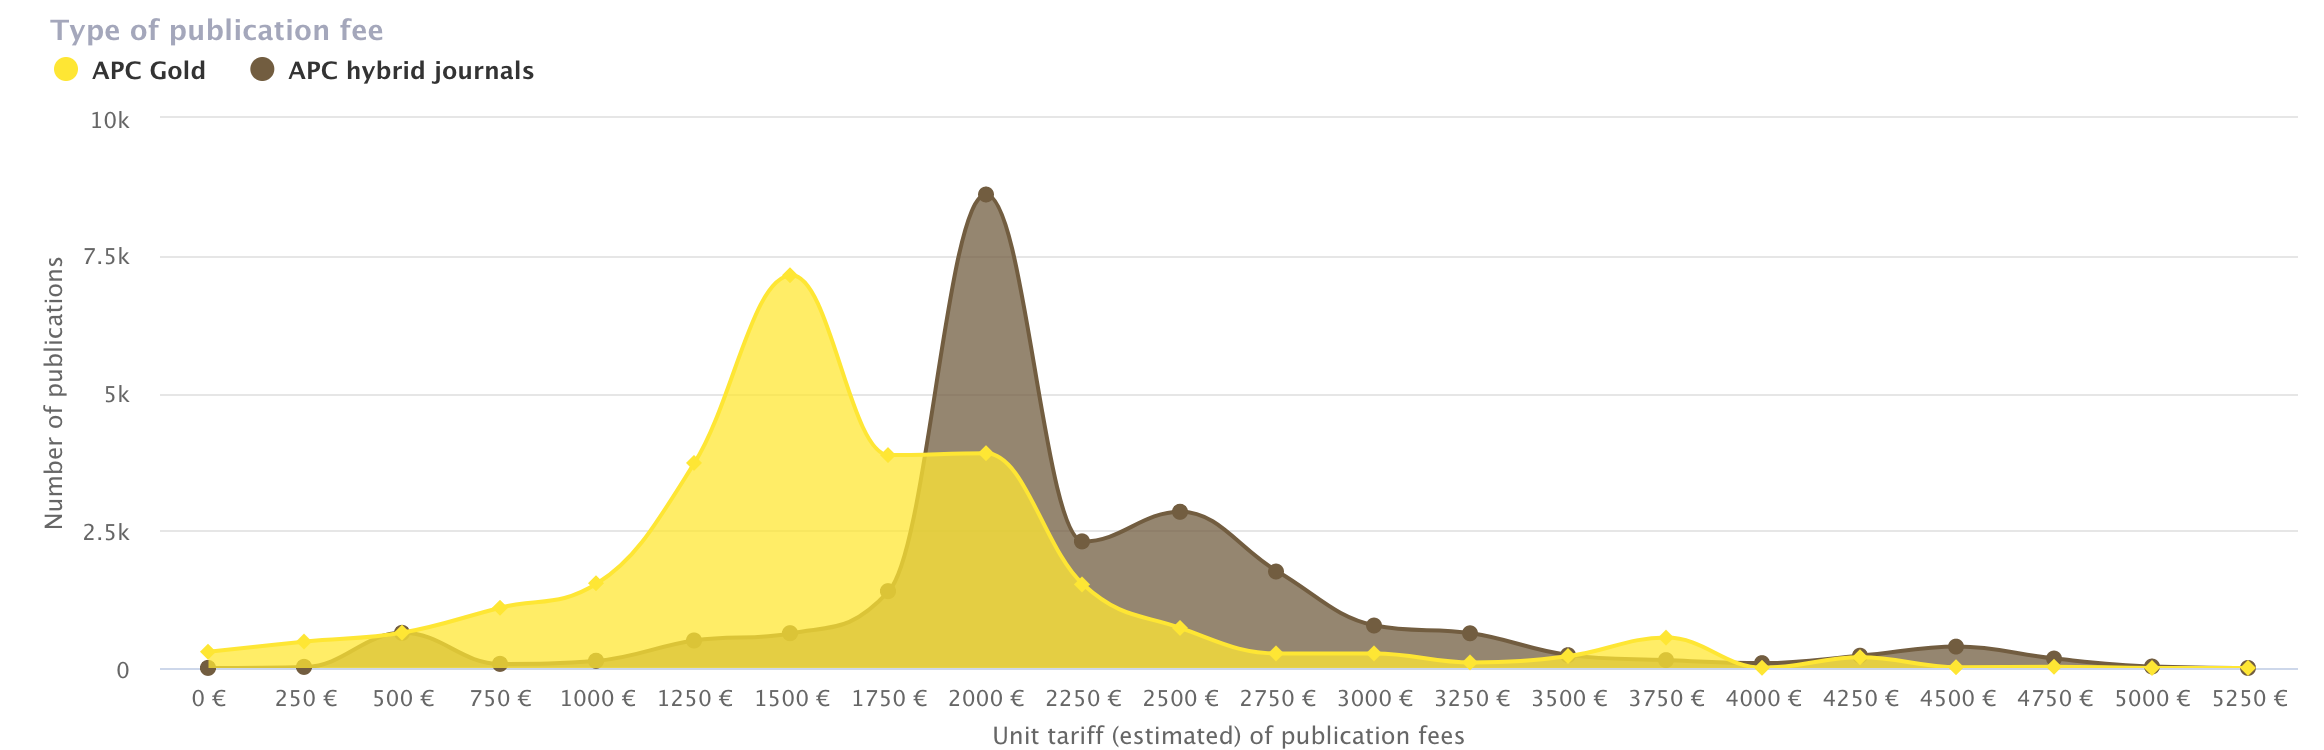
\includegraphics[width=6.25in,height=\textheight]{https://raw.githubusercontent.com/dataesr/bso-publications/main/doc/results_publications_publishers_8.png}
\caption{Distribution of scientific publications in France released in
2020 according to publication costs}
\end{figure}

\hypertarget{open-repositories-impact-on-the-open-access-dynamics}{%
\subsubsection{3.1.4 Open repositories impact on the open access
dynamics}\label{open-repositories-impact-on-the-open-access-dynamics}}

The open repositories are open access platforms on which scientific
publications are deposited, which can be consulted by anyone. They are
most often powered by author deposit, but in some cases may be powered
by the journal publishers themselves. Open archives perform different
functions: they make articles published in subscription journals
available in open access, they ensure the permanent preservation of
scientific literature and facilitate the identification of the outputs
of a laboratory or an institution. Several incentives have led to an
increase in the number of French scientific publications deposited in an
open archive. This is mandatory for publications from projects funded by
the ANR since 2019. The monitor also counts the preprints servers among
open archives, on which researchers deposit initial versions of their
manuscripts to propose them for peer review, before formal submission to
a journal.

\newpage

For each year of observation since 2018, the graph represents the share
of scientific publications in France released during the previous year
that are available in an open archive. Some of these publications may be
simultaneously made available in open access by their publisher. Thus,
in 2021, 46\% of scientific publications in France released in 2020 were
available in an open archive (figure 24).

\begin{figure}
\centering
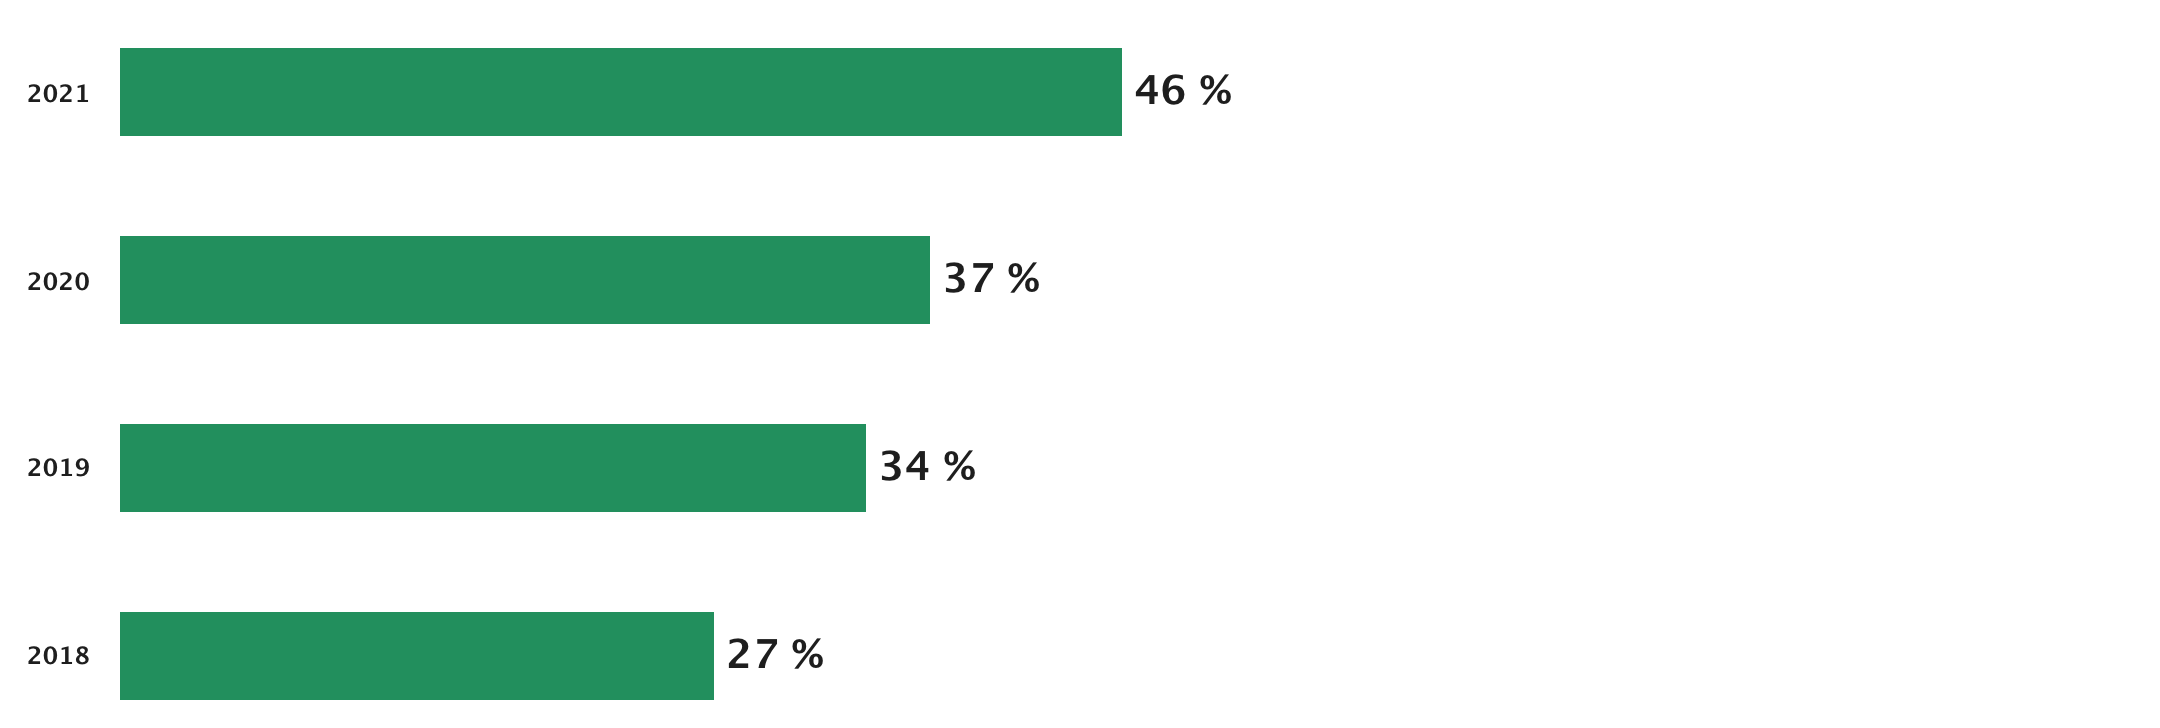
\includegraphics[width=6.25in,height=\textheight]{https://raw.githubusercontent.com/dataesr/bso-publications/main/doc/results_publications_repo_1.png}
\caption{Rate of scientific publications in France available in an open
archive by observation date}
\end{figure}

In the figure 25, for each observation date and by publication year, the
rate of scientific publications in France that are available in an open
archive. Each line represents the rates observed for an observation date
and each rate is expressed as a function of the volume of publications
published in the year observed. We observe that, for publications
released during a given year, the availability rates in an open archive
progresses from one observation year to the next. This is due to the
fact that authors of publications progressively proceed to deposit them
in an open archive, in particular when embargoes imposed by publishers
have expired. Thus, between 2018 and 2021, the rate of publications
released in 2017 that are available in an open archive has increased
from 27\% to 38\%.

\begin{figure}
\centering
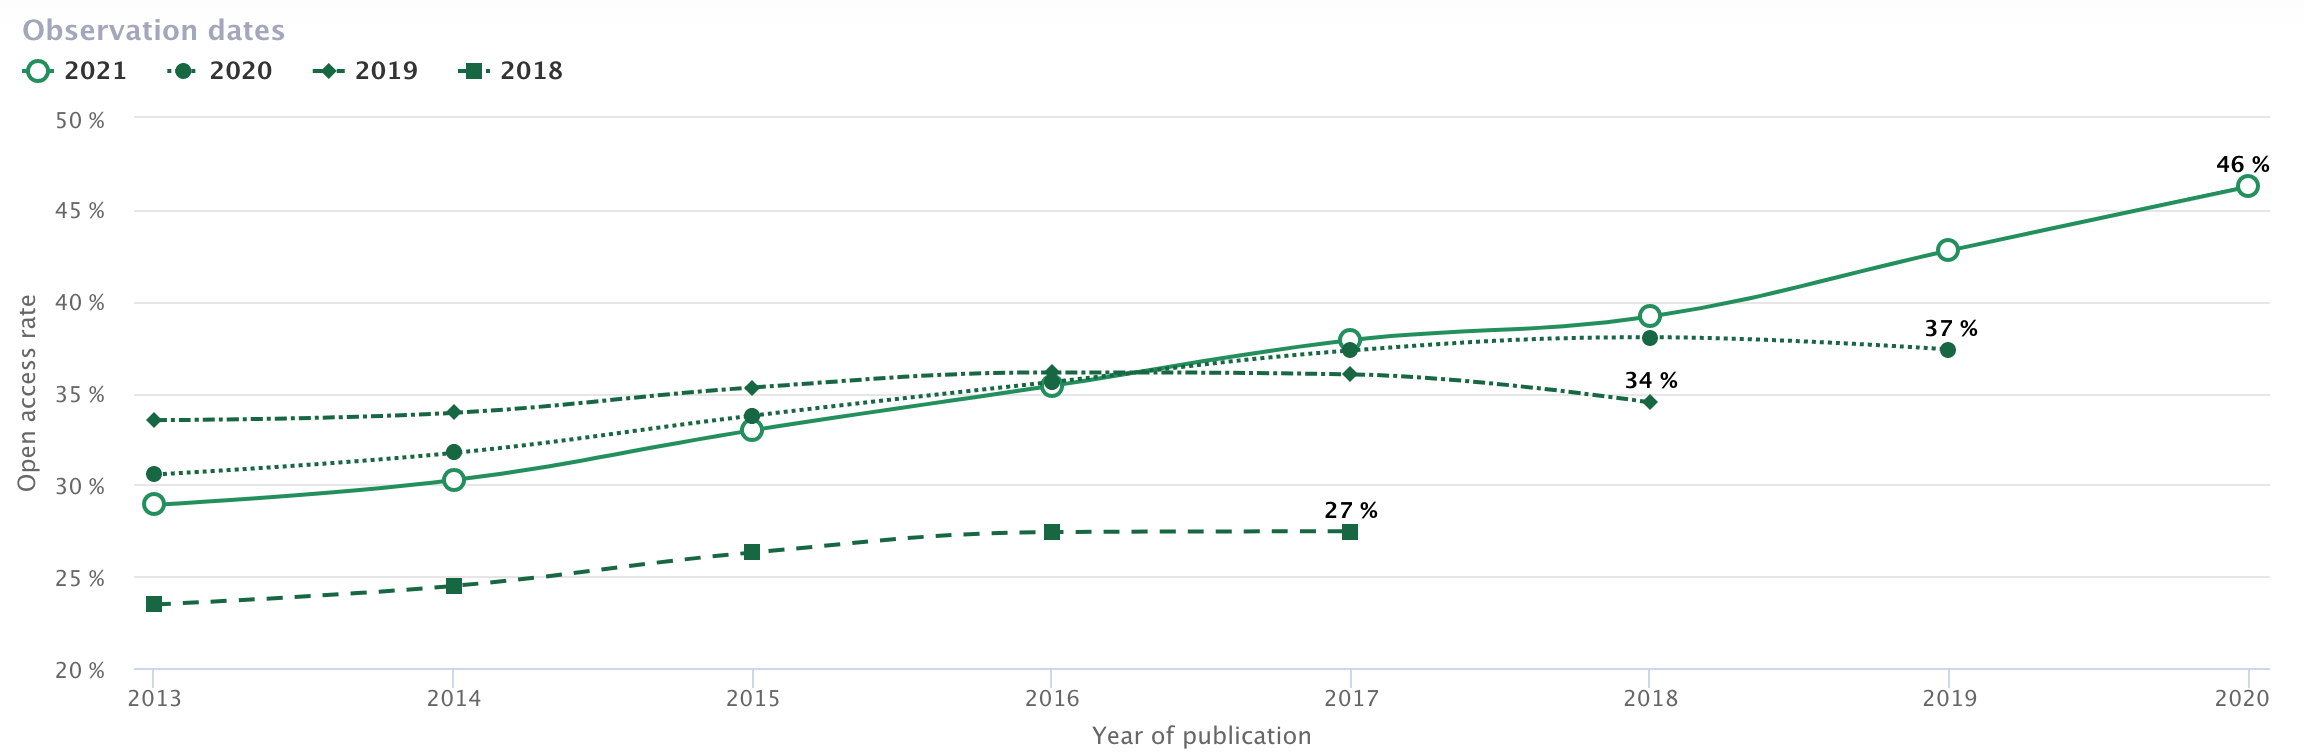
\includegraphics[width=6.25in,height=\textheight]{https://raw.githubusercontent.com/dataesr/bso-publications/main/doc/results_publications_repo_2.png}
\caption{Evolution of the rate of scientific publications in France
available in an open archive, by observation date}
\end{figure}

HAL, Pubmed Central, ArXiv and BioRxiv are the archives that hosted the
most French publications in 2020. Several factors explain the choice by
researchers of an open archive to deposit their publication. Some
archives are references in a discipline (PubMed Central (PMC) for
medical research), others are focused on the scientific production of a
country (HAL for France). A single publication can be deposited
simultaneously in several open archives. The deposit in open archives of
foreign research institutions is due to the presence of co-authors who
are affiliated with them.

The figure 26 indicates which are the most used open archives hosting
scientific publications in France published in 2020, specifying for each
the number of publications concerned. When the same publication is
deposited on several open archives, it is counted several times. In
particular, it can be seen that HAL hosts 37,335 publications within the
scope in 2020. The open archive HAL (all disciplines) is thus the main
open archive used for scientific publications in France, well ahead of
PubMed Central (biomedicine), arXiv (physics, mathematics and computer
science) and bioRxiv (biology).

\begin{figure}
\centering
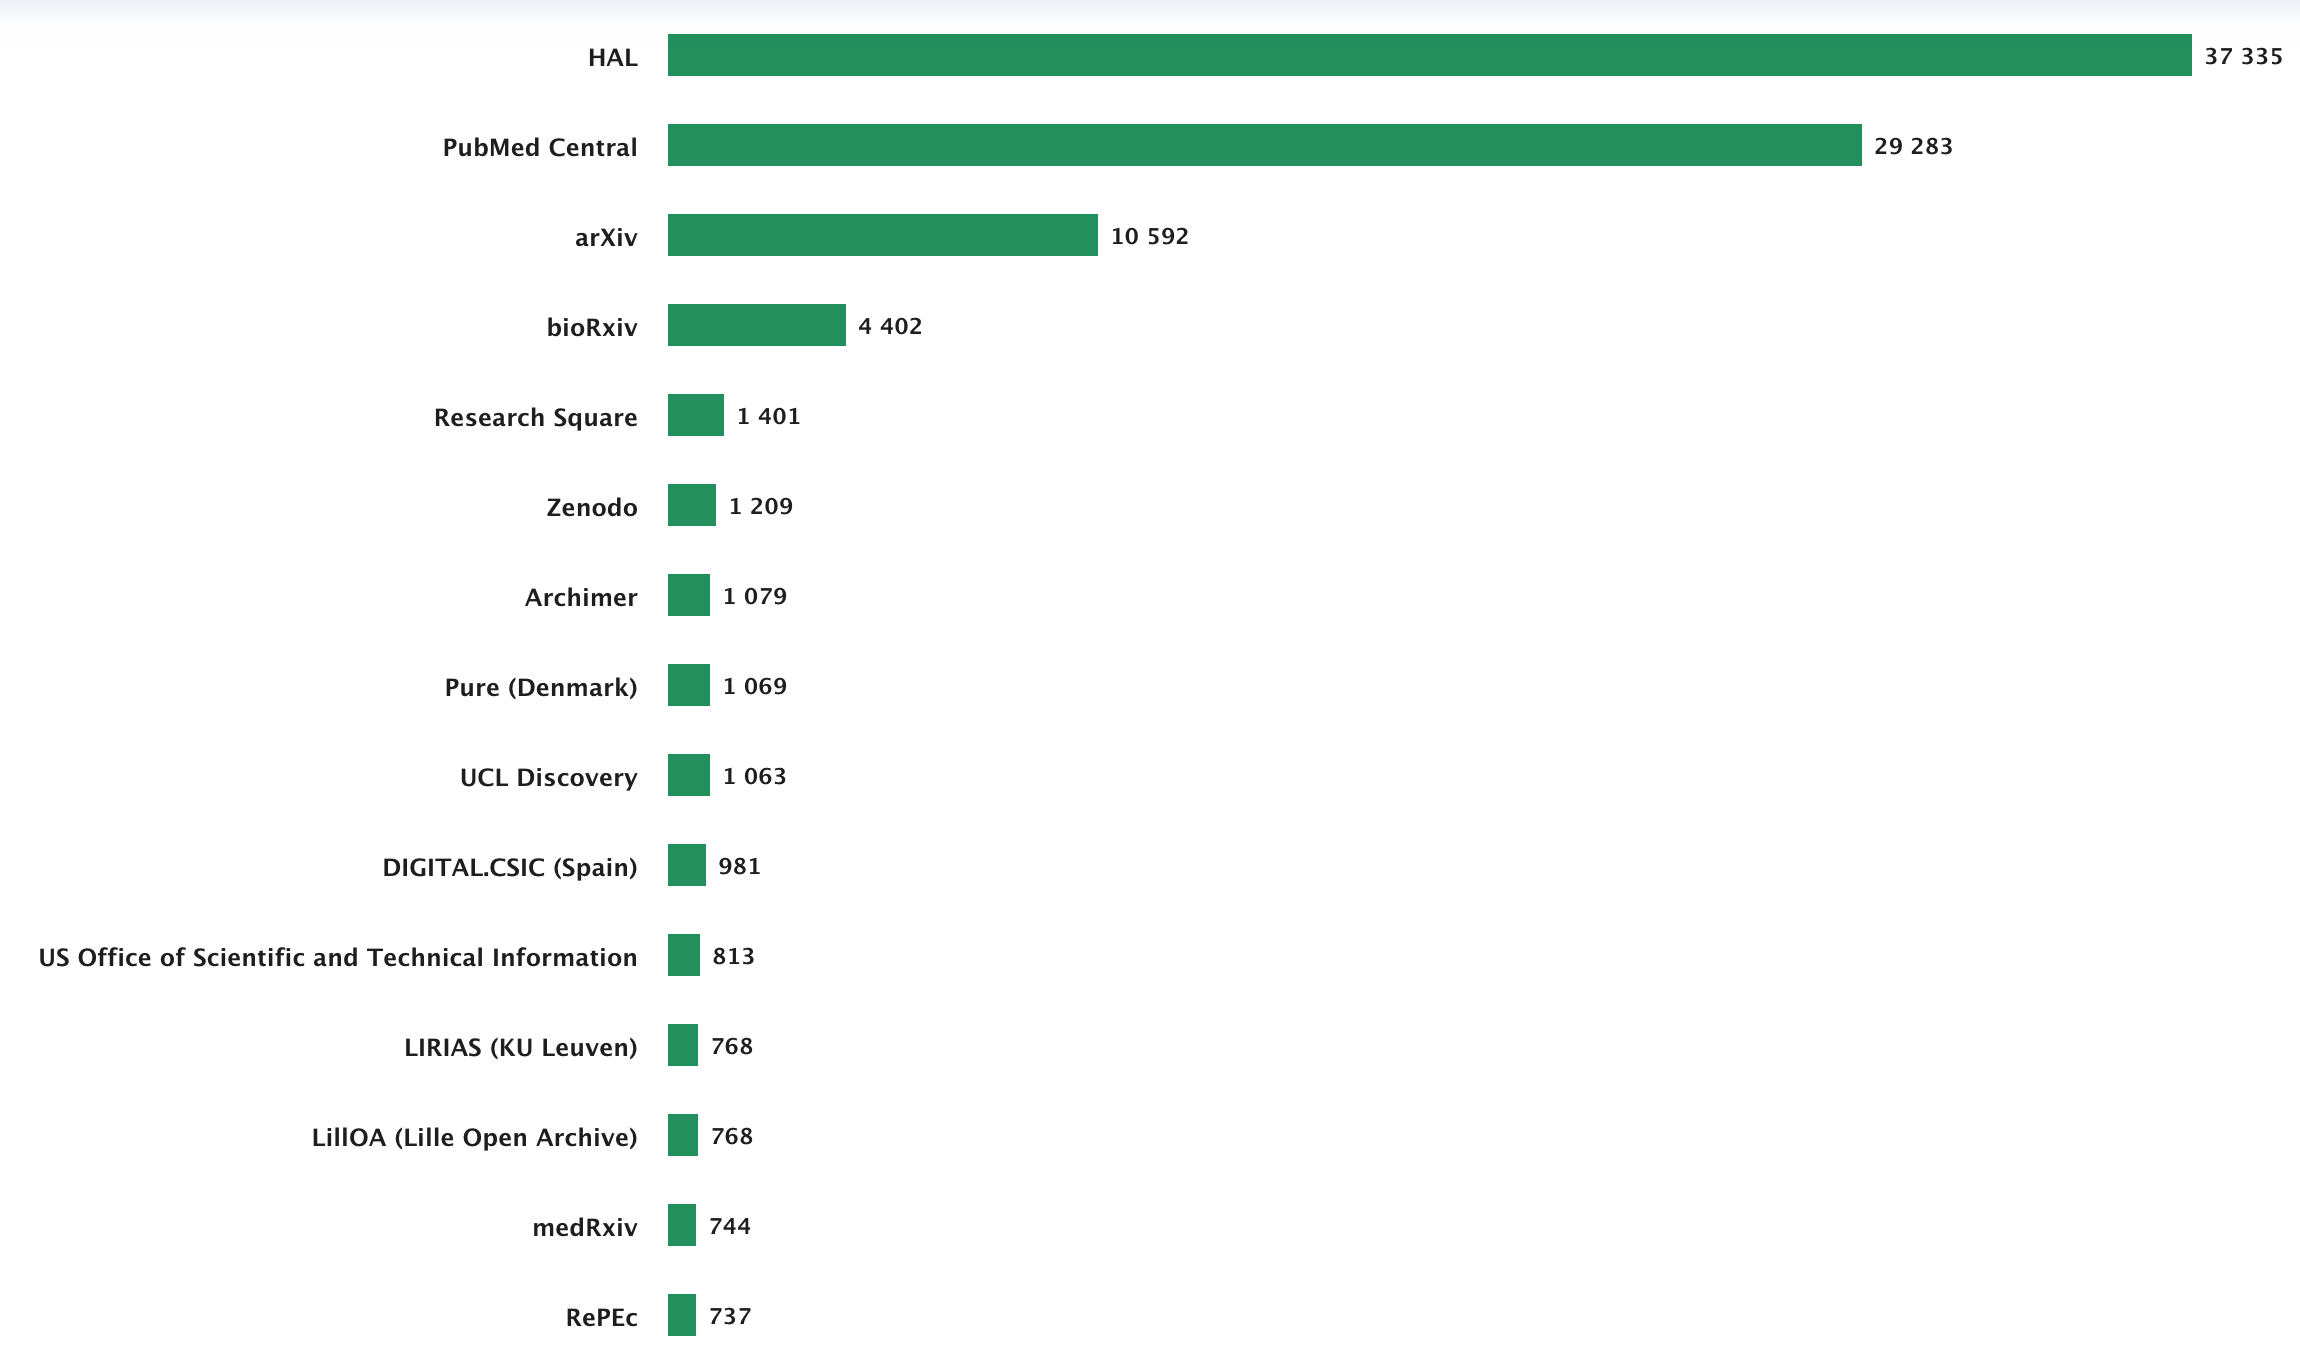
\includegraphics[width=6.25in,height=\textheight]{https://raw.githubusercontent.com/dataesr/bso-publications/main/doc/results_publications_repo_3.png}
\caption{Main open archives hosting scientific publications in France
published in 2020}
\end{figure}

HAL is a multidisciplinary open archive that hosts mostly French
scientific publications (at least one France-based author)- although its
scope is not limited to them. It is intended to play the role of a
national archive for French research, guaranteeing both free access to
scientific publications and their preservation. However, HAL is not the
only open archive used by French researchers: depending on their
institutional context or their disciplinary practices, they may prefer
to deposit on other platforms, in particular when they have a global
disciplinary audience. Therefore, the setting up of processes allowing
to reference and to integrate in HAL French scientific publications
deposited on other open archives is an important development axis.

HAL is the main open archive used to open French scientific
publications. The figure 27 indicates among the scientific publications
in France available on an open archive, the proportion of those
available on HAL, by year of publication, as observed in 2021. We see in
particular that among the scientific publications in France released in
2020 and opened on an archive, 48\% are available on HAL (and thus 52\%
are not available on HAL but on at least one other archive or preprint
server).

\begin{figure}
\centering
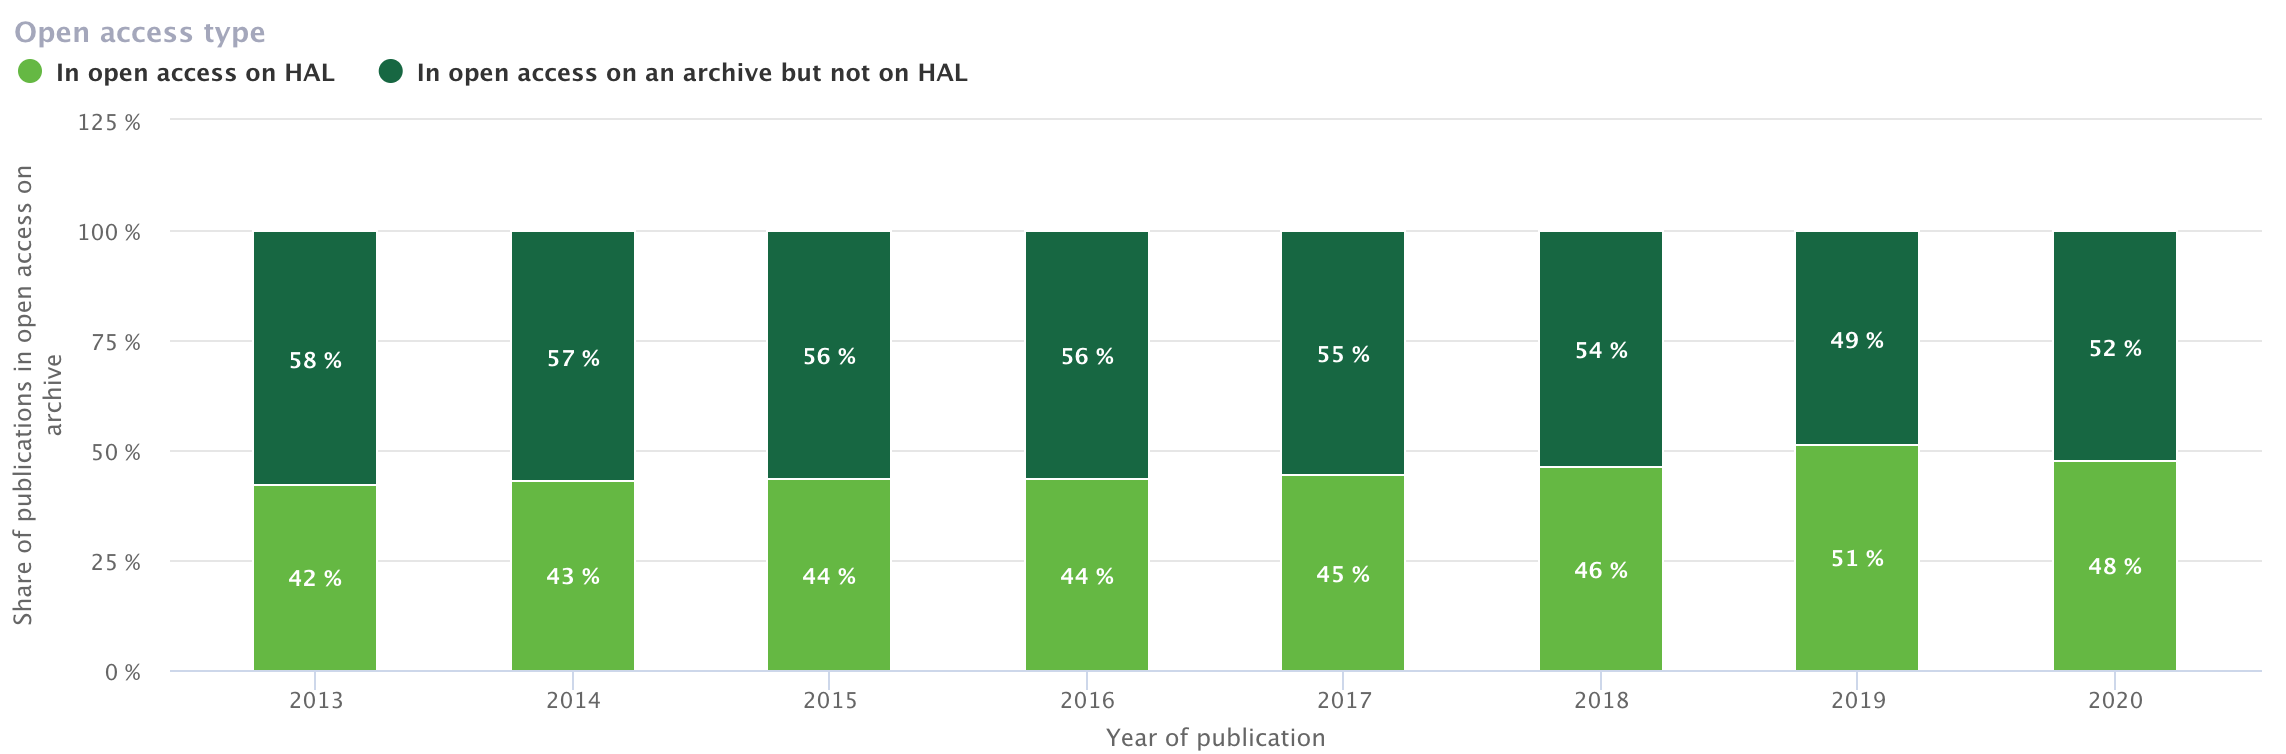
\includegraphics[width=6.25in,height=\textheight]{https://raw.githubusercontent.com/dataesr/bso-publications/main/doc/results_publications_repo_4.png}
\caption{HAL coverage rate on scientific publications in France
available in an open repository}
\end{figure}

\newpage

\hypertarget{open-access-in-france-in-the-biomedical-field}{%
\subsection{3.2 Open access in France in the biomedical
field}\label{open-access-in-france-in-the-biomedical-field}}

All the above indicators are detailed for the biomedical field. We
simply apply the same computations rules on the publications that are
indexed in PubMed.

\begin{figure}
\centering
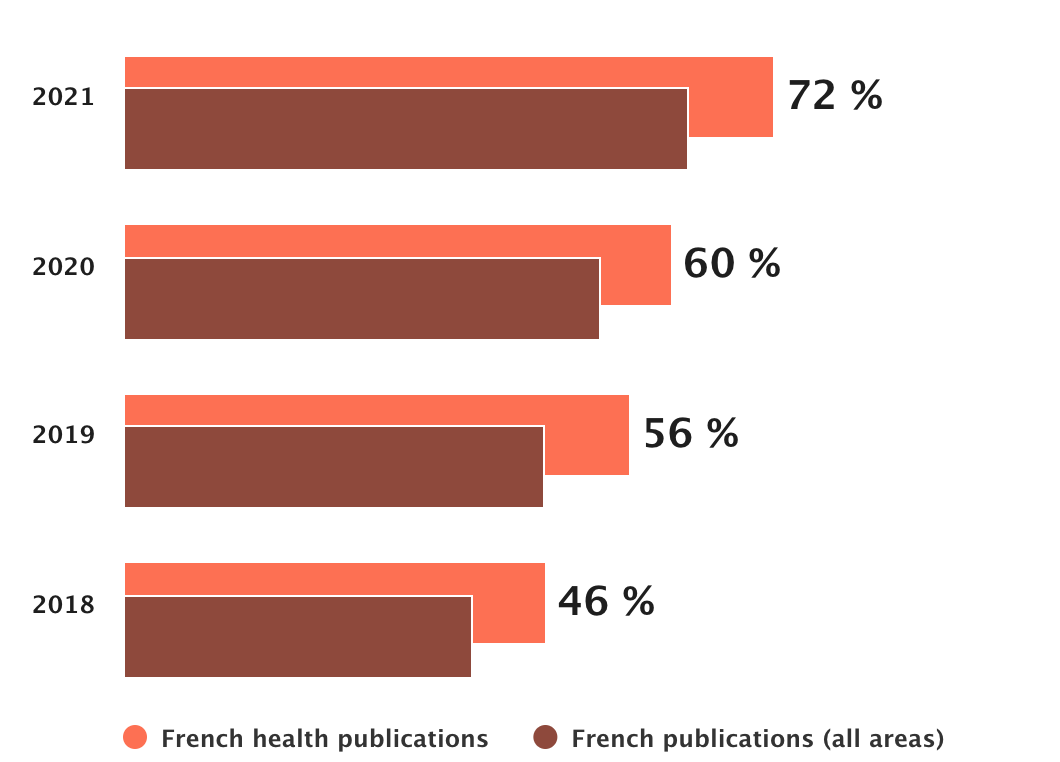
\includegraphics[width=3.64583in,height=\textheight]{https://raw.githubusercontent.com/dataesr/bso-publications/main/doc/results_publications_health_1.png}
\caption{Open access rate of scientific publications in France in health
published during the previous year by observation date}
\end{figure}

\hypertarget{clinical-trials-transparency-in-france}{%
\subsection{3.3 Clinical trials transparency in
France}\label{clinical-trials-transparency-in-france}}

The clinical trials are research conducted on human beings, involving an
intervention other than their usual care (delivery of a drug, use of a
medical device, surgical act, etc.) in order to develop biological or
medical knowledge. The lead sponsor of a clinical trial, who initiates,
finances and supervises its conduct, may be a public or private
organization: a health institution, a research organization, a
pharmaceutical company, a medical device manufacturer, etc. The Open
Science Barometer takes into account French clinical trials, i.e.~those
in which at least one of the participating institutions is located in
France.

The registration of clinical trials and their results in public
databases contributes to greater transparency in medical research. It
allows a rapid circulation of results, even when these have been
unsuccessful and are not the subject of a scientific publication. It
avoids the duplication of trials, verifies the methodology used and
increases the confidence of the patients involved. It also attests to
the proper use of funds allocated to medical research. The World Medical
Association's Declaration of Helsinki, which defines the ethical
principles applicable to medical research involving human subjects,
establishes since 2008 that all clinical trials should be registered in
a public database before the first patient is enrolled and that the
results should be made public. These principles have also been supported
since 2006 by the World Health Organization. Registries exist to carry
out these registrations: ClinicalTrials.gov, an American registry that
lists many studies conducted outside the United States, and the EU
Clinical Trials Register in the European Union. Other registries exist
but are not taken into account here because of their much lower use. In
EU countries, the reporting of the results of clinical trials involving
drugs within 12 months of their completion was made mandatory by a 2014
regulation, which came into force on January 31, 2022, the date the
Clinical Trials Information System (CTIS) became operational. This
requirement does not apply to non-drug clinical trials. The analyzes
presented do not take into account clinical trials that are not
registered in a public registry, the number of which is not known. The
registration of clinical trials in a public registry should not be
confused with prior declarations made to the competent authorities, such
as ethics committees, to obtain authorizations to conduct these trials.
These are not public.

The figure 29 represents, for all clinical trials conducted in France
that have been registered and reported as completed in a public registry
since 2010, those for which results have been communicated in this same
registry. This communication may take the form of a compilation of the
results obtained (we speak of ``posted'' results), a scientific
publication (we consider them ``published'' results) or both. We do not
introduce any hierarchy between posted results and published results. In
both cases, they are considered as results communication. The graph
distinguishes between clinical trials which sponsor is an industrial
company (industrial sponsor) and those whose sponsor is a public
research institution (academic sponsor). The graph does not take into
account clinical trials that are not registered in a public registry. In
France, the share of completed clinical trials that have posted and/or
published results of publications is estimated at 57\%. Industrial
sponsors have much more systematic practices of transparency of their
results (76\%) while public sponsors share their results much less
(31\%).

\begin{figure}
\centering
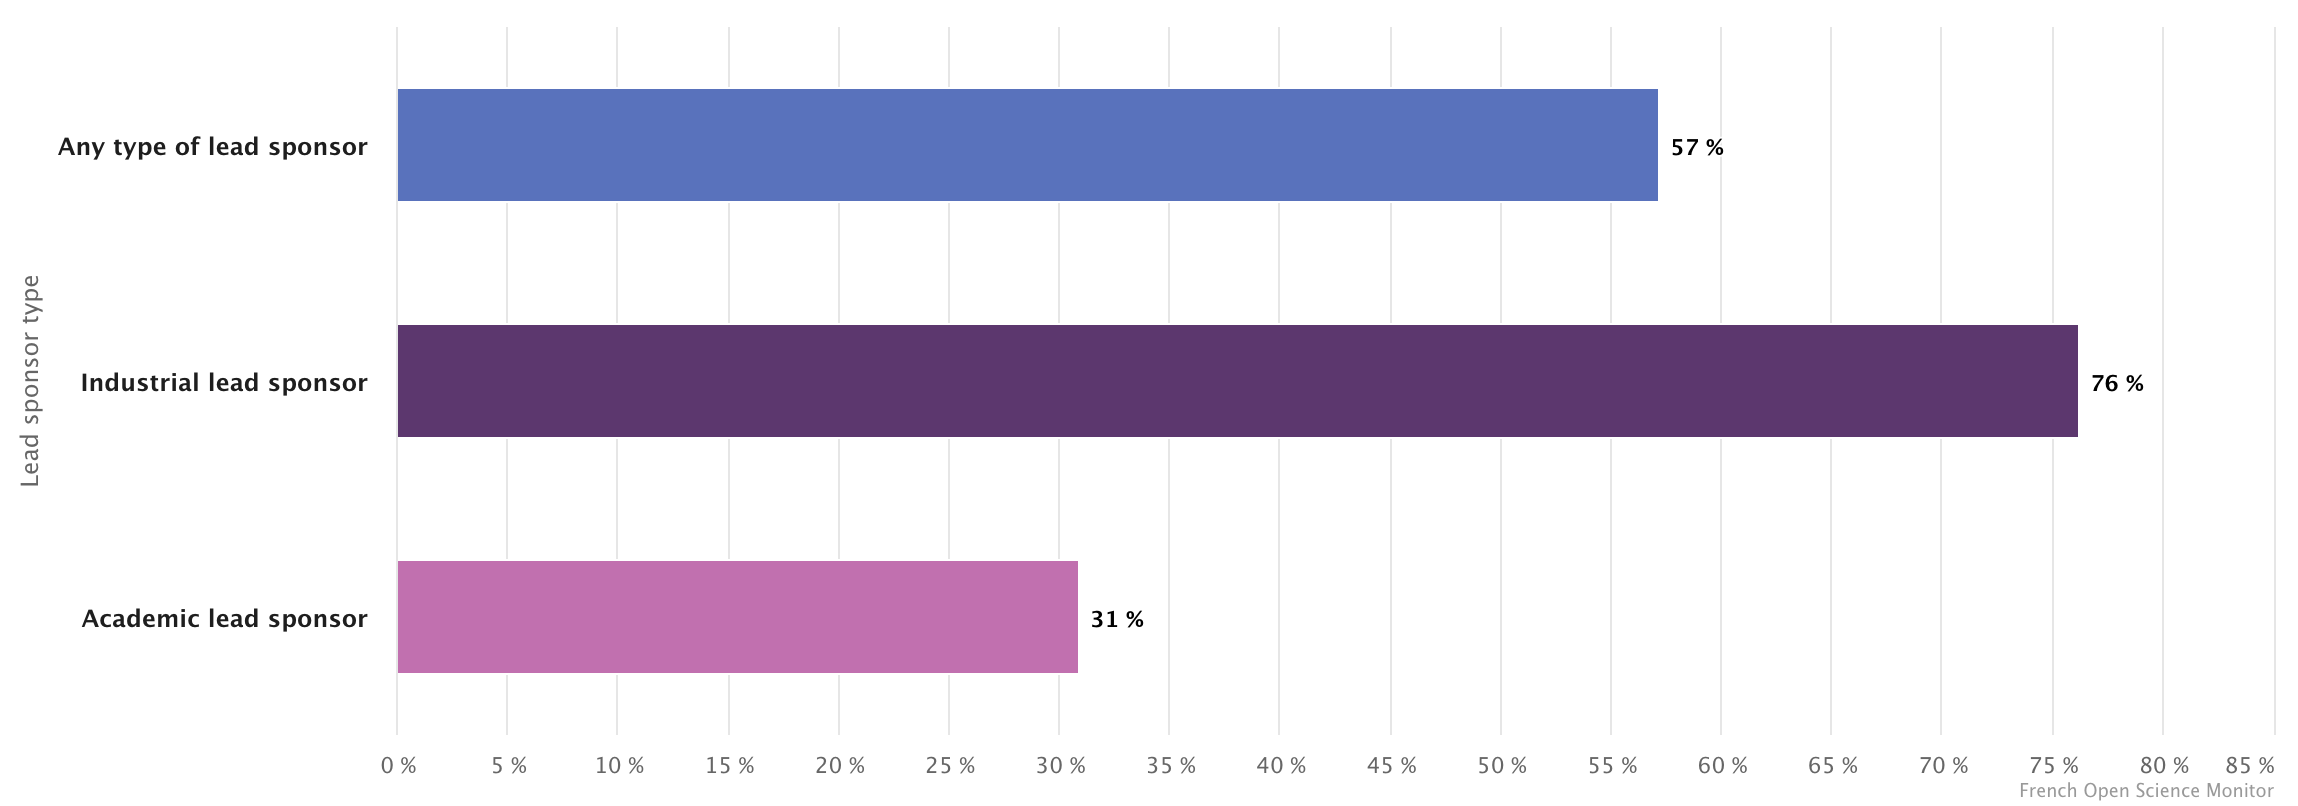
\includegraphics[width=6.25in,height=\textheight]{https://raw.githubusercontent.com/dataesr/bso-publications/main/doc/results_ct_1.png}
\caption{Share of registered and completed clinical trials that have
posted or published results}
\end{figure}

The figure 30 must be read from left to right. It presents, for all
clinical trials conducted in France that have been registered and
reported as completed in a public registry since 2010, those for which a
result has been posted or published. When a result has been reported,
the graph distinguishes between those that are posted and those that are
published in a peer-reviewed scientific publication. Finally, when a
publication is mentioned, it specifies whether or not it is available in
open access.

\begin{figure}
\centering
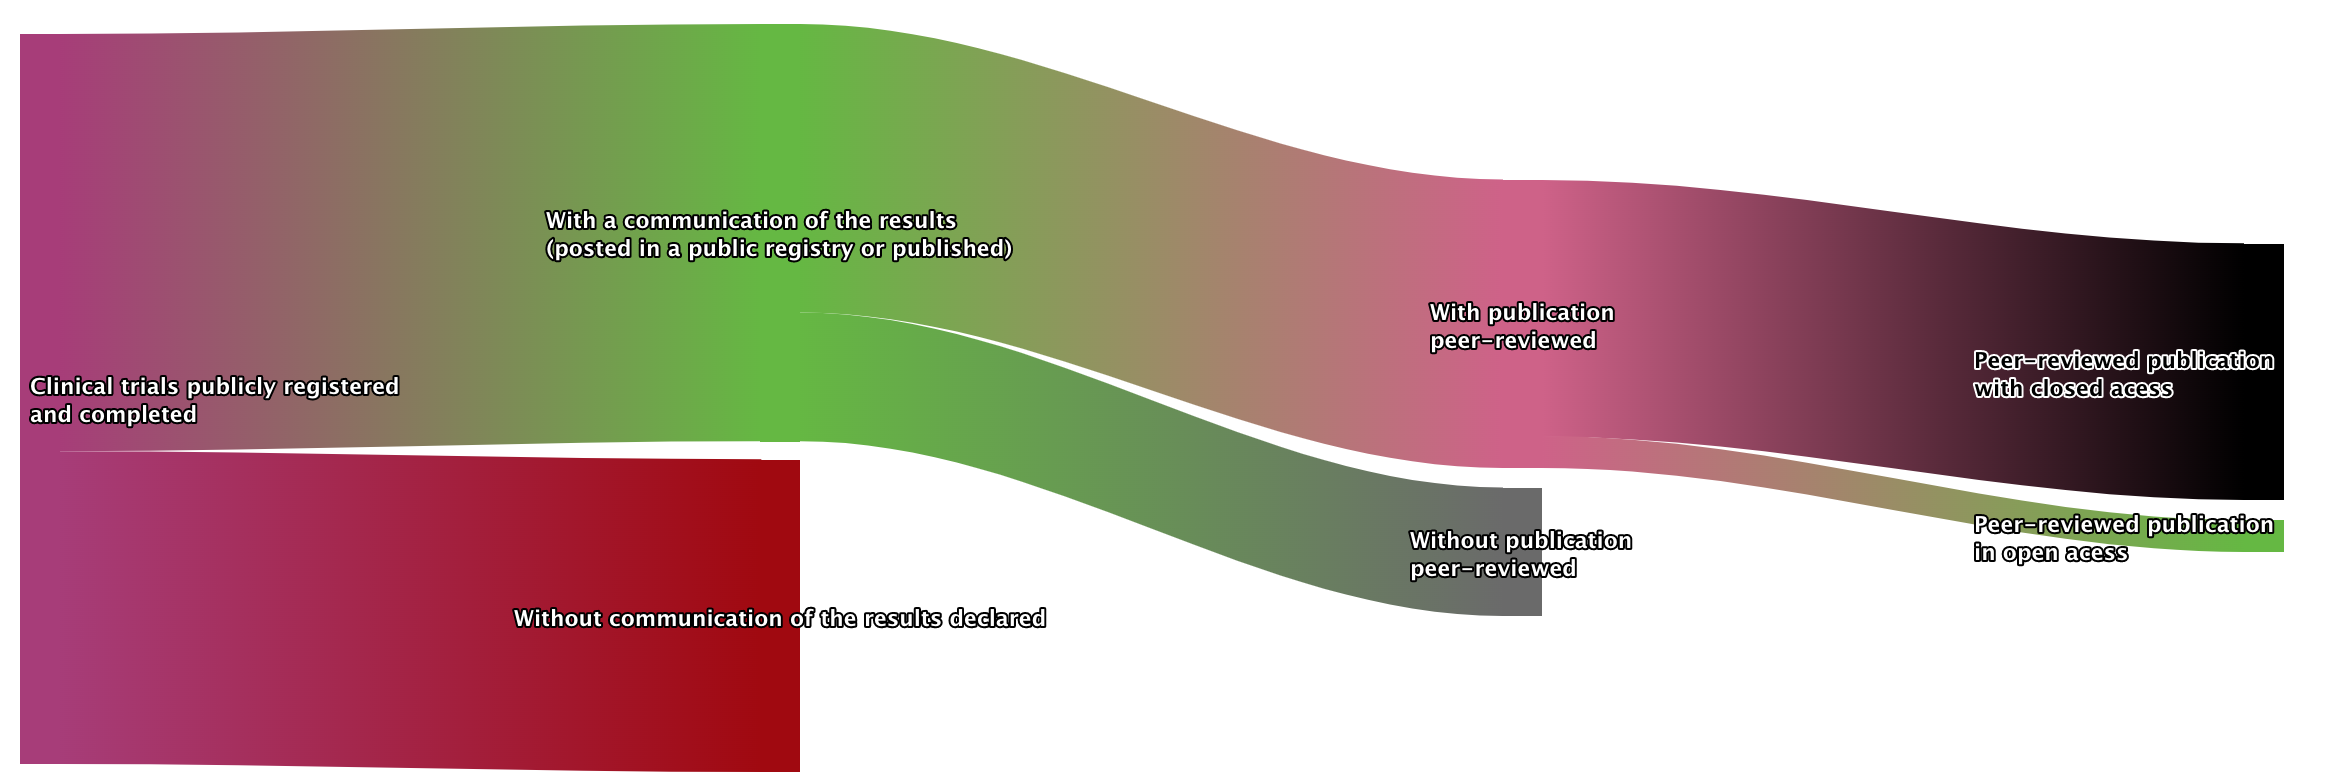
\includegraphics[width=6.25in,height=\textheight]{https://raw.githubusercontent.com/dataesr/bso-publications/main/doc/results_ct_2.png}
\caption{Distribution of clinical trials by results reporting}
\end{figure}

The World Medical Association (WMA)'s Declaration of Helsinki
(Association (n.d.)) states that the dissemination of results from
medical research involving human beings, is an ethical obligation for
all those involved, whether researchers, sponsors or publishers of
scientific journals. Indeed, it appears to be a necessary counterpart to
the involvement of patients in such research and as a major scientific
and public health issue. The dissemination of results may take the form
of an article in a scientific journal (published results) or a summary
in a clinical trial register (posted results). This second vector
ensures that the results of negative or inconclusive clinical trials,
which are difficult to value in a scientific publication, are made
public and properly disseminated. They are indeed valuable scientific
contributions and the trials from which they result should not be
ignored or unnecessarily duplicated.

\begin{figure}
\centering
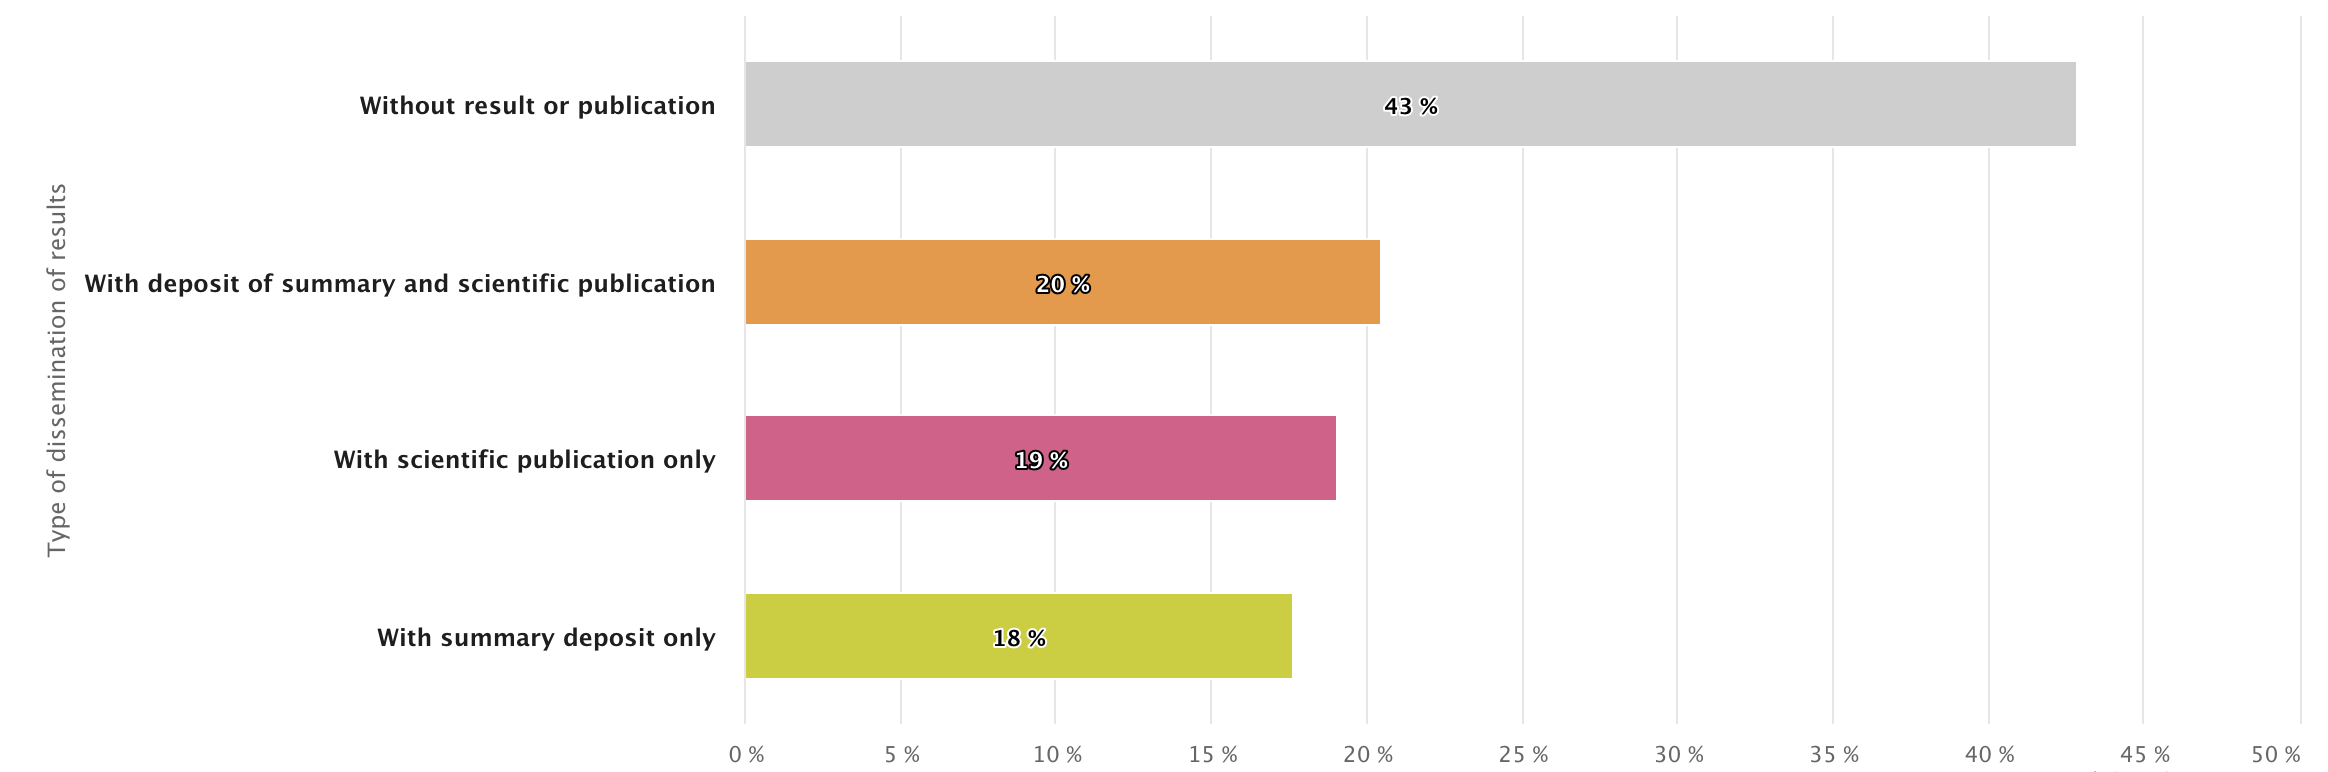
\includegraphics[width=6.25in,height=\textheight]{https://raw.githubusercontent.com/dataesr/bso-publications/main/doc/results_ct_3.png}
\caption{Procedures for reporting the results of completed clinical
trials}
\end{figure}

Responsible sharing of individual data from clinical trials is a major
challenge for the scientific community: sharing these data allows great
transparency and maximizes the value of the data collected with the
realization: • of re-analyzes with the aim of verifying the conclusions
of the trials, • secondary analyzes exploring new research questions
based on existing data, • meta-analyzes on individual data which, by
pooling different studies exploring the same question, make it possible
to provide the most precise answer possible. The International Committee
of Medical Journal Editors (ICMJE) has stated that the responsible
sharing of clinical trial data is ethically justified (Zarin et al.
(2017)): since research subjects are willing to take risks for uncertain
individual benefits, they expect the best possible use of the data
collected, while minimizing the risk of re-identification. The ICMJE
therefore requires that a data sharing statement specifying the terms of
any sharing be included in each publication from July 1, 2018, and that
it be specified in advance during clinical trial registration from
January 1, 2019. At this point, data sharing is recommended by the ICMJE
but is not a requirement.

The figure 32 shows the number of registered clinical trials with and
without individual data sharing statements by year since 2010. There has
been a slow increase in the use of this instrument: 4\% in 2010 and 17\%
in 2021.

\begin{figure}
\centering
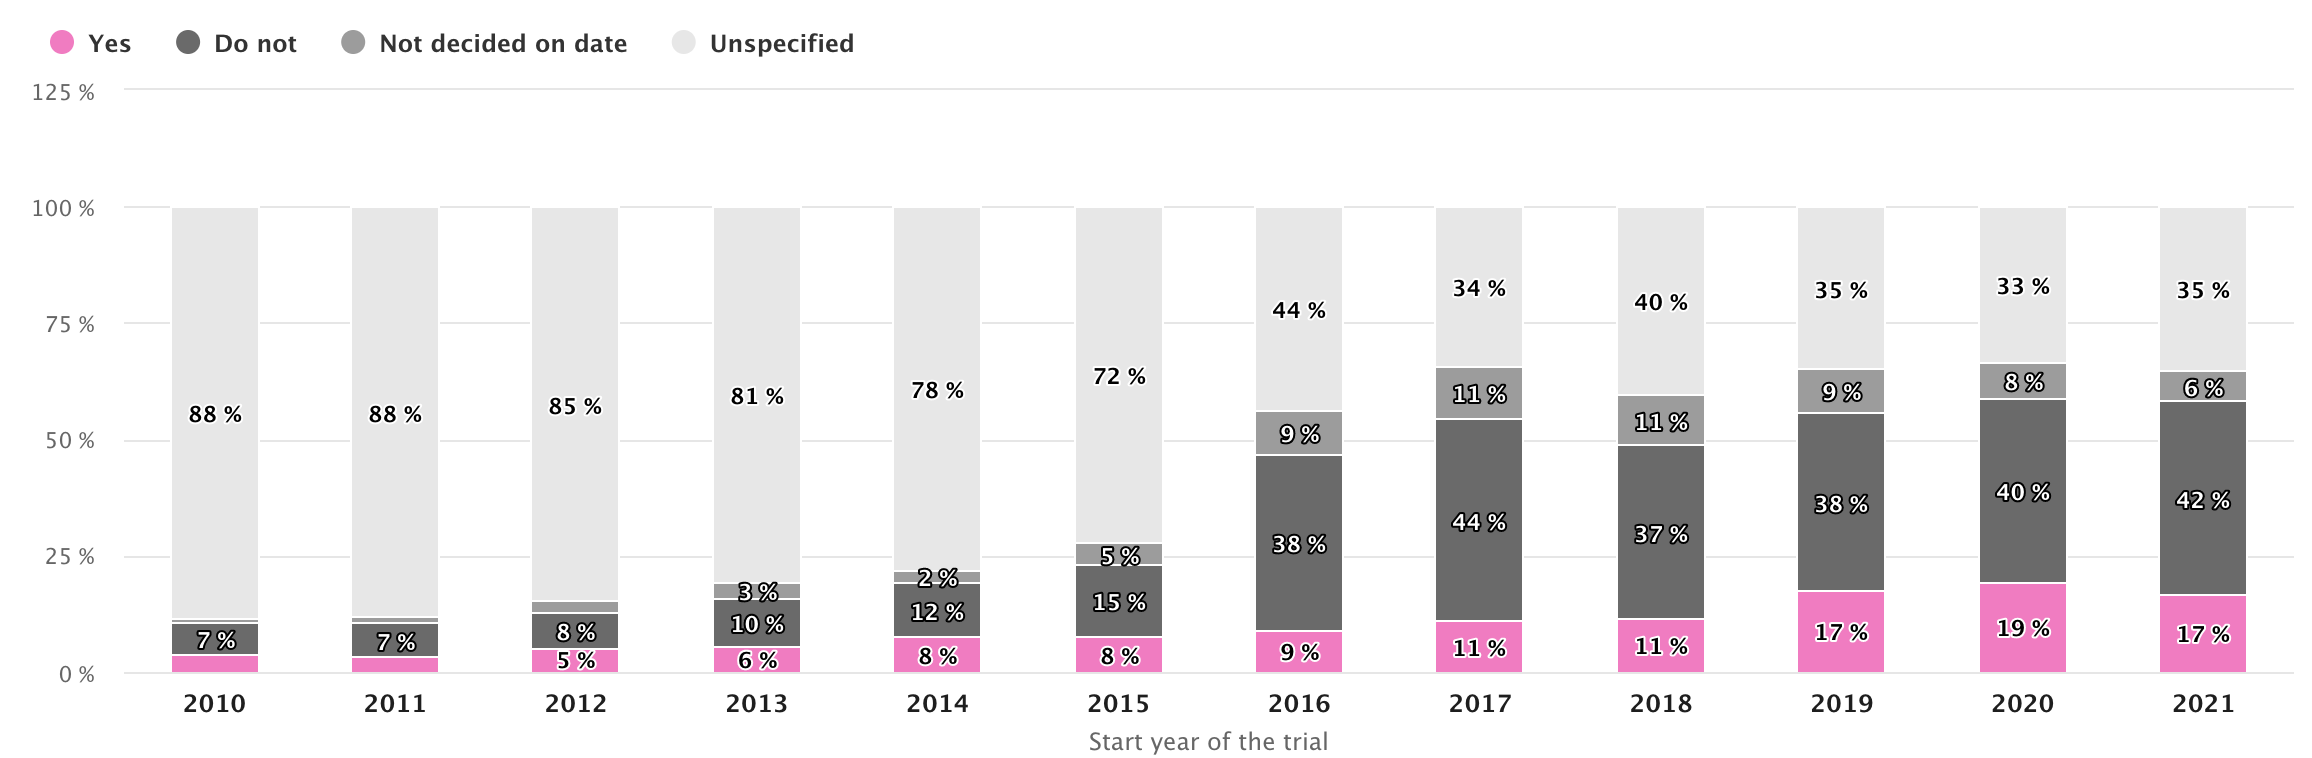
\includegraphics[width=6.25in,height=\textheight]{https://raw.githubusercontent.com/dataesr/bso-publications/main/doc/results_ct_4.png}
\caption{Distribution of registered clinical trials by presence of a
data sharing statement}
\end{figure}

Observational studies are research studies conducted on human beings
that do not involve any intervention other than their usual care, for
example by questionnaires, cohort studies, etc. The legislation does not
make it compulsory to publish the results of observational studies.
However, a prior registration and systematic publication of the results
of observational studies, on the same model as clinical trials, is a
good practice that we are trying to measure. For the current version of
the monitor, we work only on observational studies registered on the
ClinicalTrials.gov or EU Clinical Trial Register platforms, with a
methodology comparable to the one used for the clinical trials monitor.
However, our object of study is different and more difficult to capture
as many observational studies are not registered on these platforms.
These results shall therefore be analyzed with caution.

As with clinical trials, the registration of studies and publication of
their results is an important contribution to open science.

For this edition of the monitor, we estimate that 23\% of observational
studies publish results, with greater transparency from industrial
sponsors (39\%) than from public sponsors (17\%).

\begin{figure}
\centering
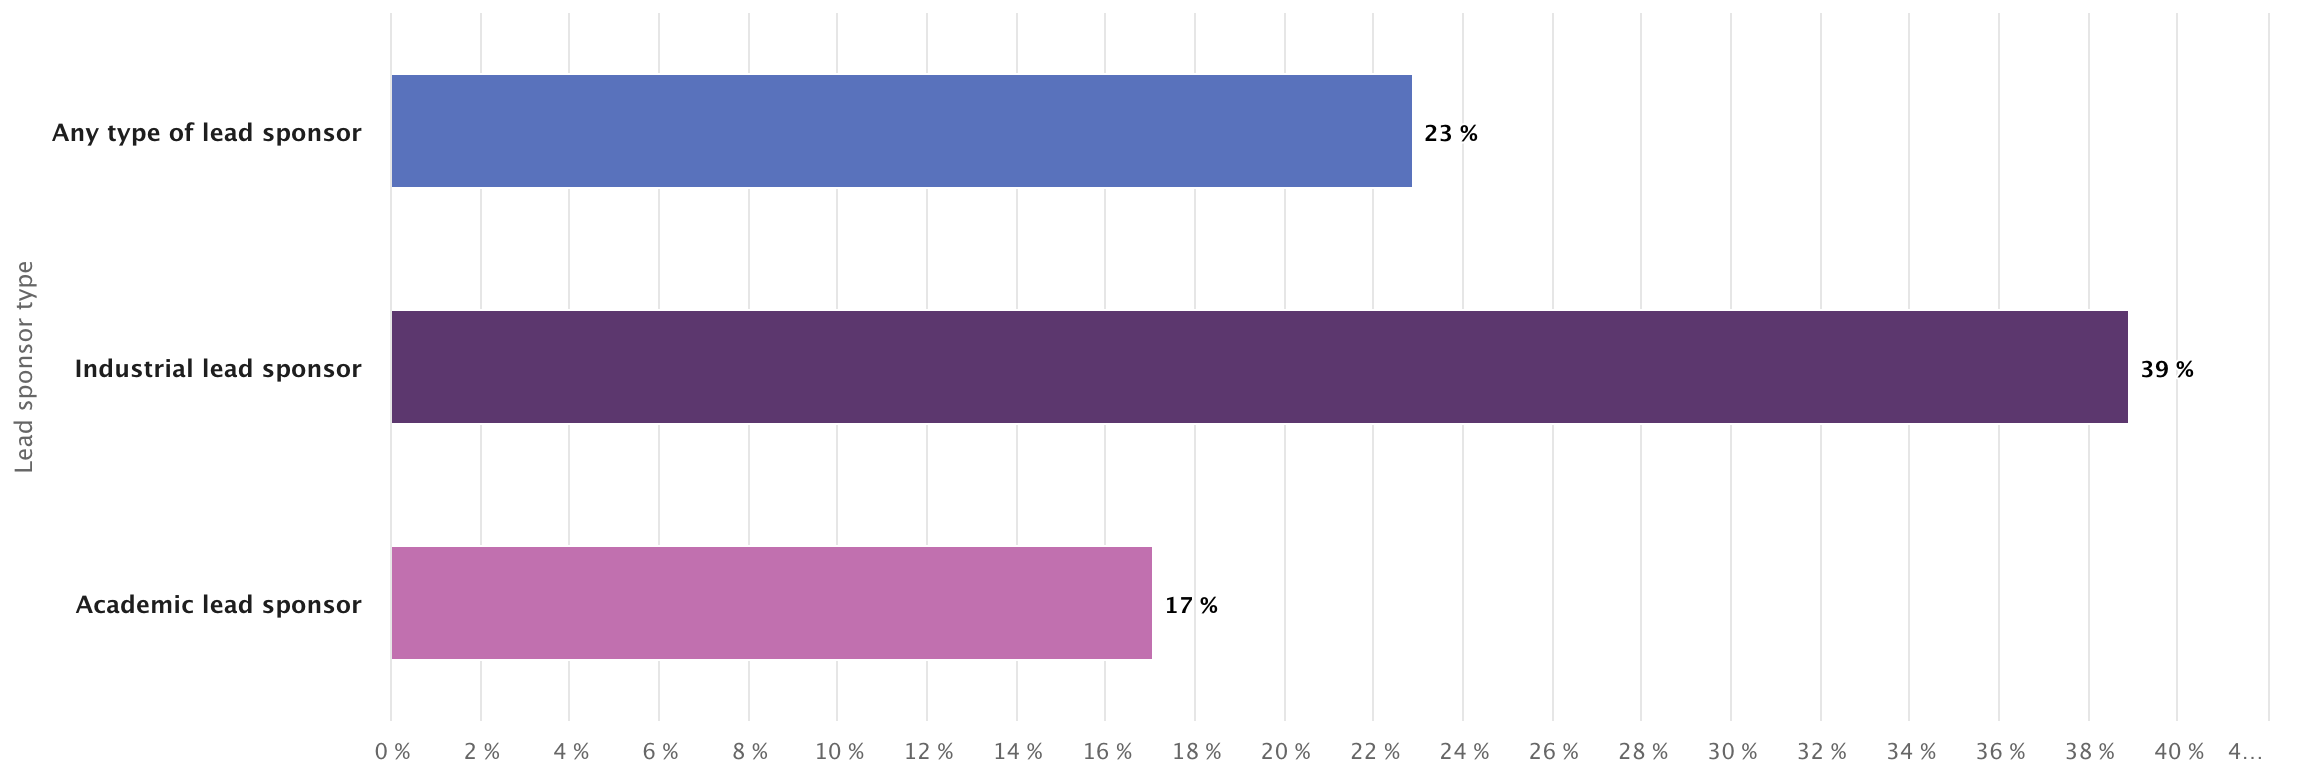
\includegraphics[width=6.25in,height=\textheight]{https://raw.githubusercontent.com/dataesr/bso-publications/main/doc/results_os_1.png}
\caption{Share of registered observational studies reporting results
between 2010 and 2020}
\end{figure}

\hypertarget{limitations-and-future-research}{%
\subsection{3.4 Limitations and future
research}\label{limitations-and-future-research}}

\hypertarget{limitations}{%
\subsubsection{3.4.1 Limitations}\label{limitations}}

The main limitation of the current approach for the publications is the
restriction to Crossref DOI. Indeed, we know it hides a fraction of the
publications, especially in the Humanities, Social sciences and Computer
sciences. This limitation is due to the fact that we need, first, to use
identifiers to count the lowest number of duplicates possible in the
monitor. Introducing Crossref-DOI-less entities would imply to set up a
proper methodology to remove potential duplicates. On top of that, we
would need an exteended OA discovery tool, as Unpaywall only focuses on
Crossref DOI. Ideally, we would also wish to have past snapshots of this
extended tool to be able to keep on producing a dynamic analysis of the
open access trends.

Another limitation of the current approach is that we mix up preprint
servers and open repositories. Both of them host open access version of
articles, but they play very different roles in scholarly communication.
Moreover, the monitor does not currently account for potential links
between preprint and published article. So, an article with a preprint
with a crossref DOI d1 and then published with another DOI d2 will
actually counts twice in the current methodology. However, this
phenomenon remains very limited as preprints represent less than 3\% of
the publications in the monitor database, especially because of the
crossref DOI restriction. arXiv announced they will set DOI on their
documents, but it will be Datacite DOI and not Crossref DOI.

\hypertarget{future-work-and-local-implementation}{%
\subsubsection{3.4.2 Future work and local
implementation}\label{future-work-and-local-implementation}}

A new generation of French Open Science Monitor is being developed in
order to integrate new research output to go beyond publications and
clinical trials. In particular, we are working on research data and
softwares. This project is led by the University of Lorraine, the French
Ministry of Higher Education, Research and Innovation, and Inria and is
supported by the European Union.

The current national-level Open Science Monitor has already been adapted
to the level of an higher education and research institutions. To date,
some twenty higher education and research institutions have already used
it to obtain reliable and open indicators on the progress of open
science in their academic production.

\hypertarget{software-and-code-availability}{%
\section{Software and code
availability}\label{software-and-code-availability}}

The source code used for the French Open Science Monitor is available on
GitHub, and shared with an open licence. The code is split in modules
for harvesting and parsing
\url{https://github.com/dataesr/harvest-pubmed} and
\url{https://github.com/dataesr/bso-parser-html}, country and
affiliation matching \url{https://github.com/dataesr/matcher},
discipline inference \url{https://github.com/dataesr/scientific_tagger},
indicators computations
\url{https://github.com/dataesr/bso-publications} and
\url{https://github.com/dataesr/bso-clinical-trials} and the web user
interface \url{https://github.com/dataesr/bso-ui}.

\hypertarget{data-availability}{%
\section{Data availability}\label{data-availability}}

The data resulting of this work is shared on the French Ministry of
Higher Education, Research and Innovation open data portal:
\url{https://data.enseignementsup-recherche.gouv.fr/explore/dataset/open-access-monitor-france/information/}
and
\url{https://data.enseignementsup-recherche.gouv.fr/explore/dataset/barometre-sante-de-la-science-ouverte/information/}.

\hypertarget{acknowledgements}{%
\section{Acknowledgements}\label{acknowledgements}}

First, we want to thank Florian Naudet
\url{https://orcid.org/0000-0003-3760-3801} from University of Rennes 1,
Rennes, France, who helped us a lot to analyze the issues related to the
clinical trials data, as well as Nicholas DeVito
\url{https://orcid.org/0000-0001-8286-1995}. We also want to thank the
agency WeDoData \url{https://wedodata.fr/} that helped us designing the
new web interface for the French Open Science Monitor.

\hypertarget{references}{%
\section*{References}\label{references}}
\addcontentsline{toc}{section}{References}

\hypertarget{refs}{}
\begin{cslreferences}
\leavevmode\hypertarget{ref-arrizabalaga_open_2020}{}%
Arrizabalaga, Olatz, David Otaegui, Itziar Vergara, Julio Arrizabalaga,
and Eva Méndez. 2020. ``Open Access of COVID-19-Related Publications in
the First Quarter of 2020: A Preliminary Study Based in PubMed.''
\emph{F1000Research} 9 (August): 649.
\url{https://doi.org/10.12688/f1000research.24136.2}.

\leavevmode\hypertarget{ref-world_medical_association_world_nodate}{}%
Association, World Medical. n.d. ``The World Medical Association-WMA
Declaration of Helsinki -- Ethical Principles for Medical Research
Involving Human Subjects.'' Accessed April 20, 2022.
\url{https://www.wma.net/policies-post/wma-declaration-of-helsinki-ethical-principles-for-medical-research-involving-human-subjects/}.

\leavevmode\hypertarget{ref-bosman_jeroen_oa_2021}{}%
Bosman, Jeroen, Jan Erik Frantsvåg, Bianca Kramer, Pierre-Carl Langlais,
and Vanessa Proudman. 2021. ``OA Diamond Journals Study. Part 1:
Findings.'' Zenodo. \url{https://doi.org/10.5281/ZENODO.4558703}.

\leavevmode\hypertarget{ref-bracco_mesurer_2022}{}%
Bracco, L. 2022. ``Mesurer L'ouverture de La Science : Le Cas de
L'Université de Lorraine.'' \emph{Revue Française Des Sciences de
L'information et de La Communication}, no. 24 (January).
\url{https://doi.org/10.4000/rfsic.12474}.

\leavevmode\hypertarget{ref-bracco:hal-03450104v1}{}%
Bracco, Laetitia. 2020. ``Baromètre Lorrain de La Science Ouverte.''
Université de Lorraine. \url{https://hal.univ-lorraine.fr/hal-03450104}.

\leavevmode\hypertarget{ref-coso_feedback_2018}{}%
COSO, French Open Science Committee. 2018. ``Feedback on EC Open Science
Monitor Methodological Note.''
\url{https://www.ouvrirlascience.fr/feedback-ec-science-monitor/}.

\leavevmode\hypertarget{ref-goldacre_compliance_2018}{}%
Goldacre, Ben, Nicholas J DeVito, Carl Heneghan, Francis Irving, Seb
Bacon, Jessica Fleminger, and Helen Curtis. 2018. ``Compliance with
Requirement to Report Results on the EU Clinical Trials Register: Cohort
Study and Web Resource.'' \emph{BMJ}, September, k3218.
\url{https://doi.org/10.1136/bmj.k3218}.

\leavevmode\hypertarget{ref-jeangirard_monitoring_2019}{}%
Jeangirard, E. 2019. ``Monitoring Open Access at a National Level:
French Case Study.'' In \emph{ELPUB 2019 23d International Conference on
Electronic Publishing}. OpenEdition Press.
\url{https://doi.org/10.4000/proceedings.elpub.2019.20}.

\leavevmode\hypertarget{ref-jeangirard_content-based_2021}{}%
Jeangirard, Eric. 2021. ``Content-Based Subject Classification at
Article Level in Biomedical Context.'' \emph{arXiv:2104.14800 {[}Cs{]}},
May. \url{http://arxiv.org/abs/2104.14800}.

\leavevmode\hypertarget{ref-joulin_bag_2016}{}%
Joulin, Armand, Edouard Grave, Piotr Bojanowski, and Tomas Mikolov.
2016. ``Bag of Tricks for Efficient Text Classification.''
\emph{arXiv:1607.01759 {[}Cs{]}}, August.
\url{http://arxiv.org/abs/1607.01759}.

\leavevmode\hypertarget{ref-laakso_delayed_2013}{}%
Laakso, Mikael, and Bo-Christer Björk. 2013. ``Delayed Open Access: An
Overlooked High-Impact Category of Openly Available Scientific
Literature.'' \emph{Journal of the American Society for Information
Science and Technology} 64 (7): 1323--9.
\url{https://doi.org/10.1002/asi.22856}.

\leavevmode\hypertarget{ref-lariviere_oligopoly_2015}{}%
Larivière, Vincent, Stefanie Haustein, and Philippe Mongeon. 2015. ``The
Oligopoly of Academic Publishers in the Digital Era.'' \emph{PLOS ONE}
10 (6): e0127502. \url{https://doi.org/10.1371/journal.pone.0127502}.

\leavevmode\hypertarget{ref-lhote_using_2021}{}%
L'Hôte, Anne, and Eric Jeangirard. 2021. ``Using Elasticsearch for
Entity Recognition in Affiliation Disambiguation.''
\emph{arXiv:2110.01958 {[}Cs{]}}, October.
\url{http://arxiv.org/abs/2110.01958}.

\leavevmode\hypertarget{ref-mesri_national_2018}{}%
MESRI. 2018. ``National Plan for Open Science.''
\url{https://cache.media.enseignementsup-recherche.gouv.fr/file/Recherche/50/1/SO_A4_2018_EN_01_leger_982501.pdf}.

\leavevmode\hypertarget{ref-mesri_2nd_2021}{}%
---------. 2021. ``2nd National Plan for Open Science.''
\url{https://cache.media.enseignementsup-recherche.gouv.fr/file/science_ouverte/20/9/MEN_brochure_PNSO_web_1415209.pdf}.

\leavevmode\hypertarget{ref-piwowar_state_2018}{}%
Piwowar, Heather, Jason Priem, Vincent Larivière, Juan Pablo Alperin,
Lisa Matthias, Bree Norlander, Ashley Farley, Jevin West, and Stefanie
Haustein. 2018. ``The State of OA: A Large-Scale Analysis of the
Prevalence and Impact of Open Access Articles.'' \emph{PeerJ} 6
(February): e4375. \url{https://doi.org/10.7717/peerj.4375}.

\leavevmode\hypertarget{ref-polonen_et_al}{}%
Pölönen, Janne, Mikael Laakso, Raf Guns, Emanuel Kulczycki, and Gunnar
Sivertsen. 2020. ``Open access at the national level: A comprehensive
analysis of publications by Finnish researchers.'' \emph{Quantitative
Science Studies} 1 (4): 1396--1428.
\url{https://doi.org/10.1162/qss_a_00084}.

\leavevmode\hypertarget{ref-waltman_ludo_scholarly_2021}{}%
Waltman, Ludo, Stephen Pinfield, Narmin Rzayeva, Susana Oliveira
Henriques, Zhichao Fang, Johanna Brumberg, Sarah Greaves, et al. 2021.
``Scholarly Communication in Times of Crisis: The Response of the
Scholarly Communication System to the COVID-19 Pandemic.'' Research on
Research Institute.
\url{https://doi.org/10.6084/M9.FIGSHARE.17125394.V1}.

\leavevmode\hypertarget{ref-zarin_update_2017}{}%
Zarin, Deborah A., Tony Tse, Rebecca J. Williams, and Thiyagu
Rajakannan. 2017. ``Update on Trial Registration 11 Years After the
ICMJE Policy Was Established.'' \emph{New England Journal of Medicine}
376 (4): 383--91. \url{https://doi.org/10.1056/NEJMsr1601330}.
\end{cslreferences}


\end{document}
